\documentclass[11pt]{article}
\usepackage[paperwidth=210mm,paperheight=280mm,margin=0.8in]{geometry}
\usepackage[T1]{fontenc}
\usepackage[utf8]{inputenc}
\usepackage{booktabs,longtable,graphicx,url,array,microtype,amsmath,amssymb,placeins}
\setlength{\emergencystretch}{3em}
\setlength{\LTpre}{6pt}
\setlength{\LTpost}{6pt}
\setlength{\tabcolsep}{3pt}
\renewcommand{\arraystretch}{1.08}
\renewcommand{\thetable}{S\arabic{table}}
\renewcommand{\thefigure}{S\arabic{figure}}
\title{Supplementary Material for\\
\emph{Timestep-Conditioned Adapter Scaling for Multi-view Diffusion Texture Generation: Control Allocation and Baked Appearance}}
\author{Anonymous authors}
\date{}
\usepackage[hidelinks]{hyperref}

\begin{document}
\maketitle
\noindent This supplement supplies complete protocols, paired results and provenance limits for the main paper's controlled study of geometry-control allocation. Fresh C, native MV-Adapter, GSO and the selected bake cohorts have separate input, interface and endpoint identities. Views and seeds are averaged within objects and do not enlarge the independent sample. Historical results and invalid attempts remain available with their original limitations.

\subsection*{Reader map: question, study identity and evidence status}
\addcontentsline{toc}{subsection}{Reader map: question, study identity and evidence status}
The main paper presents the central comparisons; the entries below locate their complete supporting records. ``Primary'' identifies a contrast within its stated protocol, not an independent replication or a shared significance family across studies. A later analysis of exposed objects remains retrospective even if its numerical calculation follows a recorded lock.

\begin{description}
\item[Executed intervention.] S1, Table~\ref{tab:supp-execution}: Fresh C's requested schedule, native group caps and post-scale correction records. These implementation records support the main method diagram and study-design table; equal applied scalar sums are not equal realized residual dose.
\item[Fresh C image controls.] S2, Table~\ref{tab:supp-freshc}: the held-out 300-object, single-checkpoint C3--Fixed Low primary and its secondary endpoints, followed by the named same-cohort addendum. Table~\ref{tab:budget300paired} supplies the retrospective equal-applied-budget pair contrasts. The original timing-allocation primary is Middle-high minus the objectwise average of Early-high and Late-high; its separate twelve-test placement family is retained. These records support the main matched-control table and neither replace that primary nor establish universal C3 superiority.
\item[Native MV-Adapter.] S3, Table~\ref{tab:mva50-paired}: fifty objects selected before new native-interface outputs, seven conditions, one specified Middle--Mean FG-PSNR primary and a separate secondary family. The objects are new to this interface, not a new Fresh C image cohort. Historical strict-276 records later in S3 have different provenance and are not pooled with this comparison.
\item[External GSO sensitivity.] S4: source-selected GSO100, native MV-Adapter, three seeds nested within each object; scheduled controls and auxiliary corrections have separately specified families. The fixed GSO20 bake study uses eleven unseen cameras per bake. Its original failure and post hoc GT-only calibration addendum remain explicit. These records support the main interface and bake-cohort tables; exposure and calibration chronology limit confirmation claims.
\item[GeoTex baked appearance.] S5, Table~\ref{tab:bake-paired}: an input-selected ten-object pilot with a specified Late--Mean LPIPS primary and four C3--Fixed High secondary tests. Old five-object and historical N=20 studies are separate. Table~\ref{tab:cross-view-all015} is the additional exploratory shared-UV family. This section supports the main bake and appearance tables, including negative results and complete rights-cleared displays.
\item[Appearance and protocol diagnostics.] S6, Table~\ref{tab:color-diagnostic}: the selected 26-object color diagnostic, followed by controlled two-object sampling, feature, resolution and branch checks. These are failure-enriched or previously observed inputs; they do not establish a validated material repair or population prevalence.
\item[Historical and auxiliary records.] S7 preserves original schedule selection, preference, FAC negatives and the retrained historical-request panel, including its condition means (Table~\ref{tab:supp-original276-means}), complete paired contrasts (Table~\ref{tab:supp-original276}), and uncertified actual-UID substitution. S8 separately reports new native training, same-base follow-up, deployment cost and projection/APG exploration. Their distinct weights, cohorts and endpoints do not supply missing historical replay or method novelty.
\item[Figure credits and study history.] S9 gives source credits and matched-view details for the supplementary displays. S10 summarizes relevant historical and auxiliary attempts; they remain separate from the current study cohorts.
\end{description}

\paragraph{How to read inference.} All confidence intervals are pointwise unless expressly stated otherwise. An adjusted $p$ value belongs only to the named family beside that result; no study-wide family is implied across separate locks. Non-detection is not equivalence, an image metric is not physical material fidelity, and selected pictures do not estimate failure prevalence. Complete positive, negative and non-detected outcomes are retained.

\tableofcontents
\clearpage
\FloatBarrier
\section*{S1. Study identities, sampling and applied-scale semantics}
\label{supp:group1}
\addcontentsline{toc}{section}{S1. Study identities, sampling and applied-scale semantics}

\subsection*{Statistical authority and reproduction map}
\addcontentsline{toc}{subsection}{Statistical authority and reproduction map}
Each numerical result in this Supplement is mapped to the internal claim ledger and scoped result sources. The original Fresh C C3--GFL primary and the later retrospective applied-budget primary have distinct object-level delta files and analysis families; requested/applied-scale records use the per-step accounting table. Layer/window and Fresh B results are maintained in separate source summaries, with Fresh B classified as retrospective sensitivity because its lock chronology cannot be authenticated from preserved Git history. The texture-complexity cohort and the color-diagnostic set are separate from Fresh C and from each other. The historical N=20 GLB-native summary has a separate analysis record; no N=20 image assets are redistributed. Original Table 9 and Table 3 below are reproduced only as historical source text with explicit provenance limits; neither is treated as a newly verified current result.

\paragraph{Portable numerical authority.} The current study summaries and source hashes are in \path{data/FACTS_round_014.json}; their endpoint and family identities must be read with the protocols below. The original retrospective applied-budget primary is reproduced in \path{data/original_applied_budget/VERIFIED_PRIMARY.json}. Its verified contrast, confidence interval, sign-flip test and all object deltas take precedence over a later summary's descriptive Middle--Fixed Mean designation. Complete pair tables and diagnostic summaries remain available with their separate inference scopes.

\paragraph{Fresh C identity details.} The 300-object Fresh C list is disjoint by UID from the original eval300, including the 24-object development probe, the 1,118-object training list, and the clean-v2 eval300. The primary four-condition run and same-cohort Generic Linear/LLH addendum use the same frozen checkpoint SHA-256 \texttt{0618d6b2\allowbreak{}84ab47aa\allowbreak{}16d7a89d\allowbreak{}c447f5ba\allowbreak{}4455ff6c\allowbreak{}9d918e5e\allowbreak{}129478a9\allowbreak{}9e0114c0}, runner source SHA-256 \texttt{e5c28e915ba137d3541eb4c032daaf62a798332d63b32917b749fe1bcc74e9e3}, cohort, input tensors, endpoint implementation, and seed policy. The seed is $42+\texttt{object\_idx}$ and is shared across the matched conditions for each object. Primary and addendum integrity gates pass for 1,200/1,200 and 600/600 condition rows. Fresh C uses the recorded deep/middle/shallow caps of 3.0/3.5/0.8, with requested, applied, and residual scales logged separately. This is a held-out paired comparison under the stated protocol. The historical identity remains explicit: 01549 names v1 weights for its main tables and a separate v2 strong-residual, per-layer-capped instance for Section 4.7/FAC. Fresh C uses a controlled retraining and is not presented as a numerical reproduction of the old Table 4 $+0.96$ dB estimate.

\subsection*{Requested/applied scale and residual-correction accounting}
\addcontentsline{toc}{subsection}{Requested/applied scale and residual-correction accounting}
Table~\ref{tab:supp-execution} lists representative Fresh C C3 records at five denoising steps. The native caps are 3.0 (deep), 3.5 (middle), and 0.8 (shallow). A cap-active fraction of 100\% means all logged records in that group/step were clipped. Raw correction $L_2$ depends on both the residual and tensor dimensions, so it is not compared across layer groups. The table instead reports the median of wrapper-level mean absolute entries, a dimension-normalized descriptive summary; differences in feature scales and distributions still prevent interpreting it as an equal-dose intervention or quality outcome. The 750-row source accounting table contains all 50 steps, three groups, and five strategies.

\begingroup\scriptsize
\begin{longtable}{c l c c c r}
\caption{Representative Fresh C requested/applied scale and post-scale residual-correction accounting. The final column is the median wrapper-level mean absolute correction entry; it is dimension-normalized but remains descriptive. Wrappers, objects, and timesteps are not independent experimental units.}\label{tab:supp-execution}\\
\toprule Step & Layer group & Requested & Applied & Cap active & Median per-wrapper mean $|c|$ \\
\midrule\endfirsthead
\toprule Step & Layer group & Requested & Applied & Cap active & Median per-wrapper mean $|c|$ \\
\midrule\endhead
0 & Deep & 1.25 & 1.25 & 0\% & 1.4786 \\
0 & Middle & 1.25 & 1.25 & 0\% & 0.3540 \\
0 & Shallow & 1.25 & 0.80 & 100\% & 0.0128 \\
12 & Deep & 1.25 & 1.25 & 0\% & 1.3969 \\
12 & Middle & 1.25 & 1.25 & 0\% & 0.4881 \\
12 & Shallow & 1.25 & 0.80 & 100\% & 0.0151 \\
24 & Deep & 2.50 & 2.50 & 0\% & 2.2588 \\
24 & Middle & 2.50 & 2.50 & 0\% & 1.1408 \\
24 & Shallow & 2.50 & 0.80 & 100\% & 0.0169 \\
37 & Deep & 1.25 & 1.25 & 0\% & 0.7513 \\
37 & Middle & 1.25 & 1.25 & 0\% & 0.4596 \\
37 & Shallow & 1.25 & 0.80 & 100\% & 0.0176 \\
49 & Deep & 1.25 & 1.25 & 0\% & 0.7354 \\
49 & Middle & 1.25 & 1.25 & 0\% & 0.1459 \\
49 & Shallow & 1.25 & 0.80 & 100\% & 0.0116 \\
\bottomrule
\end{longtable}

\endgroup

\FloatBarrier
\section*{S2. Matched GeoTex controls and complete paired statistics}
\label{supp:group2}
\addcontentsline{toc}{section}{S2. Matched GeoTex controls and complete paired statistics}

\subsection*{Original applied-budget primary and separate analysis families}\label{supp:budget-primary}
\addcontentsline{toc}{subsection}{Original applied-budget primary and separate analysis families}
The original same-cohort applied-budget protocol specified Middle-high FG-PSNR minus the objectwise mean of Early-high and Late-high. Its preserved result is $-0.0338775$ dB, median $-0.229605$ dB, pointwise percentile interval $[-0.117170,+0.051422]$, raw two-sided sign-flip $p=0.432378$, and 119/300 positive objects. The standalone verifier reproduces all 300 deltas, the exact 10,000 bootstrap draws and 20,000 sign-flip draws using seed 20261010. Middle--Fixed Mean is a separate descriptive comparison and does not replace this primary. The original twelve pairwise placement/endpoint tests use their separate Holm family. The subsequent all-pair recomputation has 50,000 resamples and a different descriptive 59-test family; its exempted Middle--Fixed Mean raw result is not the frozen primary. Neither analysis turns the exposed Fresh C addendum into independent confirmation. The original protocol, report, all 1,800 rows and twelve-test results are preserved in \path{data/original_applied_budget}; no source result is overwritten.

\subsection*{Complete Fresh C paired image-space statistics}\label{supp:freshc-complete}
\addcontentsline{toc}{subsection}{Complete Fresh C paired image-space statistics}
The original Generic Linear source manifest is delivered in \path{data/primary_studies/GENERIC_LINEAR_SOURCE_MANIFEST_shard0.json}. Its SHA256 matches the lineage record attached to the retained Generic Linear figure. Across fifty steps, deep/middle requests ramp from 1.25 to 2.50 and shallow requests from 0.50 to 0.75. All pass the stated native caps. Applied sums are (93.75,93.75,31.25), different from C3 and the equal-budget family. This is a competitive layer/time control, not a timing-only matched-dose contrast.

Table~\ref{tab:supp-freshc} reports the complete seven-endpoint paired results for C3--GFL and each of the three named addendum contrasts. The primary C3--GFL FG-PSNR result is unadjusted as the single registered primary endpoint. The six registered secondary C3--GFL endpoints use their Holm family. The addendum's FG-PSNR and FG-LPIPS contrasts use the frozen six-test primary family; the other five endpoints per contrast use the separate 15-test secondary Core-7 family. All contrasts are mean A-minus-B differences with 10,000 object bootstrap resamples and pointwise two-sided percentile 95\% CIs. Positive values favour A for PSNR/SSIM; negative values favour A for LPIPS. Adjusted $p$-values are from the frozen analysis authority. “A favourable” is the fraction of object-level differences in A's favourable direction and is descriptive.

\begingroup\scriptsize
\begin{longtable}{p{2.7cm}r l r r r}
\caption{Complete paired object-level image-space results for the primary C3--GFL contrast and the three named same-cohort addendum contrasts. Differences are A minus B; favorable-object percentages respect endpoint direction.}\label{tab:supp-freshc}\\
\toprule
Endpoint & Mean & 95\% CI & Median & A favorable & Adjusted $p$ \\
\midrule
\endfirsthead
\toprule Endpoint & Mean & 95\% CI & Median & A favorable & Adjusted $p$ \\
\midrule\endhead
\multicolumn{6}{l}{\textbf{C3 minus GFL}}\\
FG-PSNR (dB) & $+0.522$ & $[+0.404, +0.641]$ & $+0.555$ & 68.7\% & primary \\
FG-LPIPS & $-0.005345$ & $[-0.006326, -0.004403]$ & $-0.004547$ & 71.0\% & $3.2\times 10^{-22}$ \\
FG-SSIM & $+0.02453$ & $[+0.02120, +0.02805]$ & $+0.02004$ & 84.3\% & $5.9\times 10^{-33}$ \\
Edge-SSIM & $+0.004494$ & $[+0.003411, +0.005586]$ & $+0.003613$ & 69.0\% & $9.4\times 10^{-14}$ \\
Full-view PSNR (dB) & $+0.271$ & $[+0.170, +0.373]$ & $+0.220$ & 59.3\% & $4\times 10^{-07}$ \\
Full-view LPIPS & $-0.003880$ & $[-0.004926, -0.002873]$ & $-0.003029$ & 64.3\% & $8\times 10^{-13}$ \\
Full-view SSIM & $+0.005619$ & $[+0.004627, +0.006704]$ & $+0.005205$ & 83.0\% & $7.9\times 10^{-22}$ \\
\multicolumn{6}{l}{\textbf{C3 minus Generic Linear}}\\
FG-PSNR (dB) & $-0.593$ & $[-0.837, -0.351]$ & $+0.074$ & 51.7\% & $7.2\times 10^{-06}$ \\
FG-LPIPS & $+0.013512$ & $[+0.011601, +0.015487]$ & $+0.012229$ & 25.7\% & $1.3\times 10^{-32}$ \\
FG-SSIM & $-0.02810$ & $[-0.03197, -0.02439]$ & $-0.02521$ & 20.0\% & $2.9\times 10^{-35}$ \\
Edge-SSIM & $-0.010693$ & $[-0.013004, -0.008495]$ & $-0.008967$ & 33.7\% & $1.6\times 10^{-17}$ \\
Full-view PSNR (dB) & $-0.503$ & $[-0.686, -0.322]$ & $-0.139$ & 46.7\% & $2.7\times 10^{-07}$ \\
Full-view LPIPS & $-0.000897$ & $[-0.002578, +0.000862]$ & $-0.001307$ & 54.3\% & $0.611$ \\
Full-view SSIM & $+0.000046$ & $[-0.000984, +0.001011]$ & $+0.001213$ & 57.0\% & $0.927$ \\
\multicolumn{6}{l}{\textbf{LLH minus C3}}\\
FG-PSNR (dB) & $+0.621$ & $[+0.391, +0.855]$ & $-0.153$ & 46.7\% & $1.2\times 10^{-06}$ \\
FG-LPIPS & $-0.012140$ & $[-0.013861, -0.010480]$ & $-0.010837$ & 75.0\% & $9\times 10^{-34}$ \\
FG-SSIM & $+0.01658$ & $[+0.01311, +0.02003]$ & $+0.01307$ & 67.0\% & $9\times 10^{-18}$ \\
Edge-SSIM & $+0.009033$ & $[+0.006867, +0.011296]$ & $+0.006741$ & 63.3\% & $2.3\times 10^{-13}$ \\
Full-view PSNR (dB) & $+0.816$ & $[+0.639, +0.998]$ & $+0.419$ & 59.3\% & $3.2\times 10^{-16}$ \\
Full-view LPIPS & $+0.004909$ & $[+0.003266, +0.006510]$ & $+0.004538$ & 36.7\% & $3.5\times 10^{-08}$ \\
Full-view SSIM & $-0.004330$ & $[-0.005176, -0.003482]$ & $-0.004563$ & 27.7\% & $5.9\times 10^{-20}$ \\
\multicolumn{6}{l}{\textbf{LLH minus Generic Linear}}\\
FG-PSNR (dB) & $+0.028$ & $[-0.015, +0.070]$ & $+0.017$ & 52.3\% & $0.201$ \\
FG-LPIPS & $+0.001372$ & $[+0.000762, +0.002081]$ & $+0.000176$ & 46.7\% & $0.000114$ \\
FG-SSIM & $-0.01152$ & $[-0.01337, -0.00996]$ & $-0.00945$ & 8.0\% & $2.6\times 10^{-31}$ \\
Edge-SSIM & $-0.001660$ & $[-0.002096, -0.001256]$ & $-0.001648$ & 27.3\% & $1.2\times 10^{-12}$ \\
Full-view PSNR (dB) & $+0.313$ & $[+0.278, +0.347]$ & $+0.304$ & 87.3\% & $2\times 10^{-47}$ \\
Full-view LPIPS & $+0.004011$ & $[+0.003390, +0.004684]$ & $+0.003904$ & 18.0\% & $1.7\times 10^{-26}$ \\
Full-view SSIM & $-0.004284$ & $[-0.005217, -0.003543]$ & $-0.003432$ & 5.7\% & $8.5\times 10^{-20}$ \\
\bottomrule
\end{longtable}

\endgroup

\subsection*{Equal-applied-budget allocation and complete retrospective pair comparisons}
\addcontentsline{toc}{subsection}{Equal-applied-budget allocation and complete retrospective pair comparisons}
The same-cohort GeoTex addendum contains 300 objects by six conditions, 1,800 rows. Each object uses the same initial latent, input tensors and checkpoint across conditions. Early-, Middle- and Late-high use 16 high updates at 0--15, 17--32 and 34--49. Low/high are 1.25/2.50, Fixed Mean is 1.65, and the native shallow cap is 0.8. Their exact applied per-group sums are 82.5, 82.5 and 40. This comparison measures the total effect of allocating the high segment at equal applied scalar budget. Evolving residual norms are outcomes of the trajectory; lack of equal residual norms limits a mechanism interpretation, not validity of the allocation contrast. The study is post-inspection on the already evaluated Fresh C objects, not an independent confirmation.

\begingroup\scriptsize
\begin{longtable}{llll}
\caption{Selected paired contrasts from the 300-object equal-budget addendum. Mean A minus B and pointwise 95\% object-bootstrap interval (50,000 resamples). The other 59 pair--metric contrasts form one post hoc Holm family; no interval is multiplicity-adjusted.}\label{tab:budget300paired}\\
\toprule Contrast & Endpoint & Mean [95\% CI] & Holm $p$ \\
\midrule\endfirsthead
\toprule Contrast & Endpoint & Mean [95\% CI] & Holm $p$ \\
\midrule\endhead
Middle $-$ Fixed Applied Mean & fg-psnr & $-0.13326\ [-0.16979,-0.09622]$ & 1e-05 (raw) \\
Middle $-$ Fixed Applied Mean & fg-lpips & $+0.00199\ [+0.00147,+0.00254]$ & 0.00059 \\
Middle $-$ Fixed Applied Mean & fg-ssim & $-0.01185\ [-0.01347,-0.01025]$ & 0.00059 \\
Middle $-$ Fixed Applied Mean & edge-ssim & $-0.00703\ [-0.00764,-0.00643]$ & 0.00059 \\
Middle $-$ Late-high & fg-psnr & $-0.56395\ [-0.63408,-0.49427]$ & 0.00059 \\
Middle $-$ Late-high & fg-lpips & $+0.00466\ [+0.00381,+0.00553]$ & 0.00059 \\
Middle $-$ Late-high & fg-ssim & $-0.00422\ [-0.00694,-0.00139]$ & 0.01375 \\
Middle $-$ Late-high & edge-ssim & $-0.01409\ [-0.01526,-0.01291]$ & 0.00059 \\
Middle $-$ Early-high & fg-psnr & $+0.49619\ [+0.37195,+0.62282]$ & 0.00059 \\
Middle $-$ Early-high & fg-lpips & $-0.00472\ [-0.00568,-0.00378]$ & 0.00059 \\
Middle $-$ Early-high & fg-ssim & $+0.00499\ [+0.00211,+0.00809]$ & 0.00432 \\
Middle $-$ Early-high & edge-ssim & $+0.00080\ [-0.00008,+0.00170]$ & 0.1565 \\
Middle $-$ Fixed High & fg-psnr & $-0.74767\ [-0.88995,-0.60691]$ & 0.00059 \\
Middle $-$ Fixed High & fg-lpips & $+0.01070\ [+0.00889,+0.01255]$ & 0.00059 \\
Middle $-$ Fixed High & fg-ssim & $-0.04553\ [-0.04937,-0.04165]$ & 0.00059 \\
Middle $-$ Fixed High & edge-ssim & $-0.01881\ [-0.02083,-0.01678]$ & 0.00059 \\
\bottomrule
\end{longtable}\endgroup
The later recomputation exempts its named Middle--Fixed Mean FG-PSNR contrast and shows a raw $p$; the remaining 59 contrasts use its separate post hoc Holm family. This descriptive exemption is not a preregistered primary designation. The preserved original Middle--average(Early,Late) primary and twelve-test placement family are reported separately above. All are retrospective. The rank counts in main matched-budget table are not cross-metric superiority tests.

\paragraph{Default-path identity across interfaces.}
For GeoTex, explicit requested scale 1.0 and an unset scale are different: the cap is applied only when the scale attribute exists. Executing the actual wrapper with a unit residual gives deep/middle/shallow applied factors (1,1,0.8) for explicit 1.0, versus (1,1,1) when unset. The stored condition name \texttt{native\_default\_1x} therefore denotes Constant 1.0 (capped), not an unmodified pipeline. This is a wrapper-level counterexample, not a claim of full-pipeline pixel equality. In contrast, the new MV-Adapter identity gate compares three textured meshes and 18 images: official default, deployed default and a constant-1 schedule produce bitwise-identical RGB pixels, condition-encoder features and injected residuals. The 13 texture-absent MV-Adapter inputs use the documented geometry-only loader compatibility branch; their targets are constant white albedo and remain in the primary cohort.



\clearpage

\subsection*{Supporting layer/window and schedule evidence}
\addcontentsline{toc}{subsection}{Supporting layer/window and schedule evidence}
A2 is exploratory discovery evidence; A3 is a higher-dose stress regime on the same underlying cohort. A3b is a bounded Fresh B layer/window analysis. Object-cluster tests detect response heterogeneity under the tested interventions, but they do not identify a dose-independent layer-by-time mechanism or an optimal schedule.

\begin{table}[ht]
\centering\small
\caption{Object-cluster Wald interaction summaries for the tested layer-by-window maps. Cell RMSE and interaction share describe these observed maps; they are not causal effect sizes.}\label{tab:supp-layerwindow}
\begin{tabular}{lp{2.1cm}rp{4.2cm}p{2.6cm}}\toprule Map & Endpoint & Wald statistic & Interaction share; cell RMSE & Wald $p$ (A3b Holm) \\\midrule
A2 & FG-LPIPS & 481.081 & 43.5\%; 0.001695 & $8.04\times10^{-99}$ \\
A2 & FG-PSNR & 1879.963 & 56.8\%; 0.1222 dB & $<10^{-300}$ \\
A3 & FG-LPIPS & 657.237 & 11.9\%; 0.00643 & $1.14\times10^{-136}$ \\
A3 & FG-PSNR & 1389.118 & 0.8\%; 0.207 dB & $1.28\times10^{-294}$ \\
A3b & FG-LPIPS & 225.015 & 14.0\%; 0.000342 & $5.37\times10^{-43}$ \\
A3b & FG-PSNR & 525.700 & 36.0\%; 0.0205 dB & $3.43\times10^{-107}$ \\
\bottomrule\end{tabular}
\end{table}

The earlier A3b common-support calculation compared 10-step integrated raw $L_2$ norms across three layer groups. Because the saved correction tensors have different spatial resolutions (24$\times$16, 48$\times$32, and 96$\times$64) and the traces omit channel counts, absolute norms are dimension-dependent across groups. We withdraw the central-90\% intervals and 0/2,250 overlap as cross-group dose-support evidence. The earlier development calibration also used cross-layer raw $L_2$ and is not interpreted as equal-dose targeting. The fixed A3b scale values remain the tested bounded profiles. A3b remains retrospective sensitivity evidence: its map describes response heterogeneity under the tested interventions, but does not identify a dose-independent layer-by-window effect.

The separate Fresh B cohort ($N=150$) supplies schedule-location context for LLH, not evidence for C3. Table~\ref{tab:supp-freshb} preserves both registered LLH comparisons and the post-outcome HLL--LLL diagnostic. Paired intervals use 10,000 object-bootstrap resamples (seed 20261002). The LLH--LFM-EXACT intervals lie within the protocol's practical margins (FG-PSNR $\pm0.5$ dB; FG-LPIPS $\pm0.01$); this is a budget-explained interpretation within those margins, not exact equality. HLL--LLL is exploratory and its endpoint directions differ.

The Fresh B protocol-lock file states a freeze time of 2026-10-05 08:40 UTC, while the earliest preserved commit containing that file is dated 2026-10-06 00:52 UTC; its parent does not contain the file. This history does not establish when the lock was first created outside Git, but it cannot authenticate pre-run availability. Accordingly, Fresh B temporal contrasts, the A3b map, and the post-lock generic extension are treated as retrospective sensitivity evidence in this paper, even where their calculations follow the recorded comparison family. They are not described as verified preregistered confirmation.

\begin{table}[ht]
\centering\small
\caption{Fresh B paired object-level LLH comparisons, classified here as retrospective sensitivity because pre-run lock availability cannot be authenticated from the preserved history. Effects are A minus B; favorable rates respect endpoint direction. Holm values reproduce the recorded family.}\label{tab:supp-freshb}
\begin{tabular}{p{3.7cm}p{1.7cm}p{5.7cm}p{1.4cm}p{2.2cm}}\toprule Contrast & Endpoint & Mean [95\% CI] & A favors & $p$ / status \\\midrule
LLH--LFM-EXACT & FG-PSNR & +0.325 [+0.209,+0.446] dB & 54.0\% & raw $\leq0.0001$ \\
LLH--LFM-EXACT & FG-LPIPS & $-0.00460$ [$-0.00563,-0.00357$] & 76.0\% & raw $\leq0.0001$ \\
LLH--HLL & FG-PSNR & +0.687 [+0.404,+0.981] dB & 45.3\% & $\leq0.0004$; median $-0.104$ dB \\
LLH--HLL & FG-LPIPS & $-0.01098$ [$-0.01349,-0.00851$] & 80.7\% & $\leq0.0004$ \\
LLH--LLL & FG-PSNR & +0.734 [+0.597,+0.875] dB & 79.3\% & $\leq0.0004$ \\
LLH--LLL & FG-LPIPS & $-0.00845$ [$-0.01029,-0.00659$] & 82.0\% & $\leq0.0004$ \\
HLL--LLL (exploratory) & FG-PSNR & +0.047 [$-0.120,+0.208$] dB & 66.0\% & 0.5696; median +0.476 dB \\
HLL--LLL (exploratory) & FG-LPIPS & +0.00253 [+0.00155,+0.00354] & 40.0\% & $\leq0.0002$; median +0.00139 \\
\bottomrule\end{tabular}
\end{table}

The post-lock generic-schedule extension on this same Fresh B cohort is a retrospective sensitivity analysis, not independent confirmation. Table~\ref{tab:supp-generic} reports the recorded budget-matched comparisons and endpoint-matched linear counter-result. Nominal requested-scale means do not equalize post-scale residual dose; these LLH comparisons do not establish dose-adjusted schedule superiority or strengthen C3 specifically.

\clearpage
\begingroup\scriptsize
\begin{longtable}{p{3.4cm}p{1.7cm}p{4.4cm}p{1.3cm}p{2.4cm}}
\caption{Post-lock Fresh B generic-schedule extension (same $N=150$ cohort). Effects are LLH minus comparator. Budget-matched schedules form the locked eight-schedule family; endpoint-matched linear is the registered counter-comparison.}\label{tab:supp-generic}\\
\toprule Contrast & Endpoint & Mean [95\% CI] & A favors & Holm $p$ \\
\midrule\endfirsthead
\toprule Contrast & Endpoint & Mean [95\% CI] & A favors & Holm $p$ \\
\midrule\endhead
LLH--budget linear & FG-PSNR & +0.0967 [+0.0594,+0.1357] dB & 65.3\% & Holm $p\leq0.0008$ \\
LLH--budget linear & FG-LPIPS & -0.0009 [-0.0013,-0.0004] & 65.3\% & Holm $p=0.0008$ \\
LLH--budget cosine & FG-PSNR & +0.4629 [+0.3526,+0.5780] dB & 74.7\% & Holm $p\leq0.0008$ \\
LLH--budget cosine & FG-LPIPS & -0.0059 [-0.0071,-0.0046] & 80.0\% & Holm $p\leq0.0008$ \\
LLH--budget trapezoid & FG-PSNR & +0.4404 [+0.3334,+0.5521] dB & 74.0\% & Holm $p\leq0.0008$ \\
LLH--budget trapezoid & FG-LPIPS & -0.0057 [-0.0070,-0.0045] & 78.0\% & Holm $p\leq0.0008$ \\
LLH--budget Gaussian & FG-PSNR & +0.4711 [+0.3584,+0.5892] dB & 74.7\% & Holm $p\leq0.0008$ \\
LLH--budget Gaussian & FG-LPIPS & -0.0058 [-0.0071,-0.0045] & 79.3\% & Holm $p\leq0.0008$ \\
LLH--endpoint linear & FG-PSNR & -0.0373 [-0.0829,+0.0086] dB & -- & Holm $p=0.1150$ \\
LLH--endpoint linear & FG-LPIPS & +0.00109 [+0.0004,+0.0019] & -- & Holm $p=0.0024$ \\
\bottomrule
\end{longtable}
\endgroup

\clearpage

\FloatBarrier
\subsection*{Objectwise four-endpoint dominance: descriptive addendum}
\addcontentsline{toc}{subsection}{Objectwise four-endpoint dominance: descriptive addendum}
The five controls in the complete matched six-condition matrix are compared with C3 on the recorded FG-PSNR, foreground LPIPS, FG-SSIM and Edge-SSIM composite values. A control weakly dominates C3 if it is no worse on all four and better on at least one. LPIPS is reversed when forming the comparison. We use no effect threshold or fitted quality score. This is a post-inspection analysis of point estimates, not inference that every object has a resolved quality winner.

\begin{table}[ht]\centering\small
\caption{Fresh C300: all four-endpoint pairwise dominance counts. Incomparable/equal includes competing endpoint directions. Counts use the complete object matrix.}\label{tab:dominance015}
\begin{tabular}{lrrr}\toprule Control & Dominates C3 & C3 dominates & Incomparable/equal \\
\midruleFixed Low & 28 & 156 & 116 \\
Fixed High & 173 & 16 & 111 \\
Fixed Applied Mean & 143 & 4 & 153 \\
Early-high & 48 & 90 & 162 \\
Late-high & 122 & 1 & 177 \\
\bottomrule\end{tabular}
\end{table}
At least one other control dominates C3 on 270/300 objects (90.0\%; descriptive object-bootstrap interval [86.3,93.3]\%). This fraction is over the tested controls and endpoints, not the fraction with failed materials or a confidence level for overall superiority. C3 can dominate a particular fixed control while another control dominates C3. The supplied per-object Boolean matrix permits independent reconstruction of the union count. All five pairs, including cases favoring C3, are retained.

\FloatBarrier
\section*{S3. Native MV-Adapter and historical cross-interface evaluation}
\label{supp:group3}
\addcontentsline{toc}{section}{S3. Native MV-Adapter and historical cross-interface evaluation}

\subsection*{Frozen native MV-Adapter comparison on fifty new-to-interface objects}\label{supp:mva-native50}
\addcontentsline{toc}{subsection}{Frozen native MV-Adapter comparison on fifty new-to-interface objects}
The protocol was internally frozen before new scheduled outputs; it is not a public preregistration. Fifty inputs were selected in UID order from Fresh C after excluding every recorded previously inspected MV-Adapter UID. Selection uses available inputs and native geometry/material criteria, not quality or parameter search. Seeds are $20261010+\mathrm{index}$, shared across conditions. Six native-camera 512-pixel images use 50 DDPM-shift updates, CFG 3, reference strength 1 and the frozen high-quality text prompt. All 350 rows completed. Models, input identities, runner, native-target calibration and per-step residual traces are indexed in the reproduction archive.

Early-, Middle- and Late-high use high=1 over steps 0--15, 17--32 and 34--49 respectively, with low=0.75 elsewhere. Fixed Mean=0.83 and Generic Linear spans 0.75--0.91 inclusively; each sums to 41.5 per feature, whereas Native/Fixed High sums to 50 and Fixed Low to 37.5. These are feature-scaling controls on MV-Adapter, not GeoTex's per-ResNet capped residual doses.

Official/deployed default and constant-1 scheduled paths match exactly on three textured new objects, including 18 RGB images, encoded conditions and injected residuals. Native target geometry positions/masks match the control rasterization for all fifty inputs; an independent CPU bilinear source-UV sample agrees within the frozen tolerance. Thirteen texture-absent assets use geometry-only compatibility loading and white target albedo; they remain in the primary fifty. The 37-object textured subset is descriptive. It does not create a second primary or substitute after observing outcomes.

The primary Middle-high--Fixed Mean FG-PSNR mean is $+0.02899$ dB, 95\% CI $[-0.01941,+0.08074]$, Monte Carlo sign-flip $p=0.28075$ (100,000 draws, plus-one correction); 29/50 favor Middle. Intervals use 50,000 object resamples. The other 104 contrasts (21 condition pairs by five endpoints, minus primary) form one predeclared Holm family; intervals remain pointwise. No non-inferiority or architecture-causal claim follows from a non-separated contrast.

\begingroup\scriptsize
\begin{longtable}{llrr}
\caption{Complete native fifty-object pair--metric contrasts. A minus B; lower LPIPS/CIEDE2000 and higher other endpoints are favorable. $p$ is Holm-adjusted except the single primary marked raw.}\label{tab:mva50-paired}\\
\toprule A -- B & Endpoint & Mean [95\% CI] & $p$ \\
\midrule\endfirsthead
\toprule A -- B & Endpoint & Mean [95\% CI] & $p$ \\
\midrule\endhead
High -- Low & fg-psnr & $-0.12682\ [-0.24503,-0.02980]$ & 0.85601 \\
High -- Low & fg-lpips & $+0.00100\ [-0.00197,+0.00592]$ & 1.00000 \\
High -- Low & fg-ssim & $-0.00250\ [-0.00594,+0.00029]$ & 1.00000 \\
High -- Low & edge-ssim & $+0.00511\ [+0.00114,+0.00979]$ & 0.85601 \\
High -- Low & ciede2000 & $+0.44730\ [+0.13967,+0.87441]$ & 0.20880 \\
High -- Mean & fg-psnr & $-0.08309\ [-0.16282,-0.02065]$ & 0.78170 \\
High -- Mean & fg-lpips & $+0.00013\ [-0.00120,+0.00214]$ & 1.00000 \\
High -- Mean & fg-ssim & $-0.00268\ [-0.00534,-0.00051]$ & 1.00000 \\
High -- Mean & edge-ssim & $+0.00163\ [-0.00023,+0.00339]$ & 1.00000 \\
High -- Mean & ciede2000 & $+0.33298\ [+0.10737,+0.65171]$ & 0.13932 \\
High -- Early & fg-psnr & $+0.00563\ [-0.03952,+0.05131]$ & 1.00000 \\
High -- Early & fg-lpips & $-0.00158\ [-0.00243,-0.00081]$ & 0.01649 \\
High -- Early & fg-ssim & $+0.00002\ [-0.00176,+0.00171]$ & 1.00000 \\
High -- Early & edge-ssim & $+0.00228\ [-0.00040,+0.00477]$ & 1.00000 \\
High -- Early & ciede2000 & $+0.03229\ [-0.06895,+0.13756]$ & 1.00000 \\
High -- Middle & fg-psnr & $-0.11208\ [-0.22257,-0.02534]$ & 0.89608 \\
High -- Middle & fg-lpips & $+0.00175\ [-0.00105,+0.00664]$ & 1.00000 \\
High -- Middle & fg-ssim & $-0.00200\ [-0.00524,+0.00047]$ & 1.00000 \\
High -- Middle & edge-ssim & $+0.00562\ [+0.00250,+0.00961]$ & 0.02112 \\
High -- Middle & ciede2000 & $+0.41481\ [+0.13251,+0.81706]$ & 0.14875 \\
High -- Late & fg-psnr & $-0.14046\ [-0.25619,-0.04753]$ & 0.26910 \\
High -- Late & fg-lpips & $+0.00203\ [-0.00108,+0.00734]$ & 1.00000 \\
High -- Late & fg-ssim & $-0.00341\ [-0.00673,-0.00079]$ & 0.87002 \\
High -- Late & edge-ssim & $+0.00119\ [-0.00198,+0.00545]$ & 1.00000 \\
High -- Late & ciede2000 & $+0.47923\ [+0.17811,+0.90198]$ & 0.05490 \\
High -- Linear & fg-psnr & $-0.12216\ [-0.22718,-0.04049]$ & 0.22752 \\
High -- Linear & fg-lpips & $+0.00174\ [-0.00098,+0.00639]$ & 1.00000 \\
High -- Linear & fg-ssim & $-0.00309\ [-0.00618,-0.00068]$ & 0.90959 \\
High -- Linear & edge-ssim & $+0.00243\ [-0.00040,+0.00605]$ & 1.00000 \\
High -- Linear & ciede2000 & $+0.42004\ [+0.14924,+0.81173]$ & 0.05005 \\
Low -- Mean & fg-psnr & $+0.04373\ [-0.00118,+0.09206]$ & 1.00000 \\
Low -- Mean & fg-lpips & $-0.00087\ [-0.00381,+0.00085]$ & 1.00000 \\
Low -- Mean & fg-ssim & $-0.00017\ [-0.00118,+0.00090]$ & 1.00000 \\
Low -- Mean & edge-ssim & $-0.00348\ [-0.00757,-0.00081]$ & 0.36480 \\
Low -- Mean & ciede2000 & $-0.11432\ [-0.24502,-0.00126]$ & 1.00000 \\
Low -- Early & fg-psnr & $+0.13245\ [+0.04720,+0.24287]$ & 0.15288 \\
Low -- Early & fg-lpips & $-0.00258\ [-0.00777,+0.00036]$ & 1.00000 \\
Low -- Early & fg-ssim & $+0.00253\ [+0.00006,+0.00594]$ & 1.00000 \\
Low -- Early & edge-ssim & $-0.00283\ [-0.00657,-0.00016]$ & 1.00000 \\
Low -- Early & ciede2000 & $-0.41501\ [-0.81018,-0.14622]$ & 0.04876 \\
Low -- Middle & fg-psnr & $+0.01475\ [-0.01731,+0.04840]$ & 1.00000 \\
Low -- Middle & fg-lpips & $+0.00075\ [+0.00030,+0.00122]$ & 0.17384 \\
Low -- Middle & fg-ssim & $+0.00050\ [-0.00056,+0.00160]$ & 1.00000 \\
Low -- Middle & edge-ssim & $+0.00051\ [-0.00072,+0.00181]$ & 1.00000 \\
Low -- Middle & ciede2000 & $-0.03249\ [-0.10291,+0.03715]$ & 1.00000 \\
Low -- Late & fg-psnr & $-0.01363\ [-0.02840,+0.00083]$ & 1.00000 \\
Low -- Late & fg-lpips & $+0.00103\ [+0.00051,+0.00167]$ & 0.00800 \\
Low -- Late & fg-ssim & $-0.00091\ [-0.00156,-0.00021]$ & 0.79142 \\
Low -- Late & edge-ssim & $-0.00392\ [-0.00547,-0.00234]$ & 0.00303 \\
Low -- Late & ciede2000 & $+0.03193\ [+0.00504,+0.05951]$ & 1.00000 \\
Low -- Linear & fg-psnr & $+0.00467\ [-0.02786,+0.03373]$ & 1.00000 \\
Low -- Linear & fg-lpips & $+0.00074\ [+0.00032,+0.00118]$ & 0.09680 \\
Low -- Linear & fg-ssim & $-0.00058\ [-0.00154,+0.00033]$ & 1.00000 \\
Low -- Linear & edge-ssim & $-0.00267\ [-0.00418,-0.00118]$ & 0.10701 \\
Low -- Linear & ciede2000 & $-0.02726\ [-0.09723,+0.04844]$ & 1.00000 \\
Mean -- Early & fg-psnr & $+0.08872\ [+0.03375,+0.16183]$ & 0.07565 \\
Mean -- Early & fg-lpips & $-0.00171\ [-0.00411,-0.00028]$ & 0.42750 \\
Mean -- Early & fg-ssim & $+0.00270\ [+0.00064,+0.00545]$ & 0.78170 \\
Mean -- Early & edge-ssim & $+0.00065\ [-0.00092,+0.00210]$ & 1.00000 \\
Mean -- Early & ciede2000 & $-0.30069\ [-0.59160,-0.11032]$ & 0.02280 \\
Middle -- Mean & fg-psnr & $+0.02899\ [-0.01941,+0.08074]$ & 0.28075 (raw) \\
Mean -- Middle & fg-lpips & $+0.00162\ [-0.00005,+0.00462]$ & 1.00000 \\
Mean -- Middle & fg-ssim & $+0.00067\ [-0.00064,+0.00204]$ & 1.00000 \\
Mean -- Middle & edge-ssim & $+0.00399\ [+0.00170,+0.00764]$ & 0.00104 \\
Mean -- Middle & ciede2000 & $+0.08184\ [-0.02823,+0.20315]$ & 1.00000 \\
Mean -- Late & fg-psnr & $-0.05737\ [-0.10476,-0.01422]$ & 0.85601 \\
Mean -- Late & fg-lpips & $+0.00190\ [-0.00003,+0.00530]$ & 1.00000 \\
Mean -- Late & fg-ssim & $-0.00074\ [-0.00183,+0.00031]$ & 1.00000 \\
Mean -- Late & edge-ssim & $-0.00044\ [-0.00301,+0.00363]$ & 1.00000 \\
Mean -- Late & ciede2000 & $+0.14625\ [+0.03581,+0.27574]$ & 0.87002 \\
Mean -- Linear & fg-psnr & $-0.03907\ [-0.07392,-0.01081]$ & 0.57941 \\
Mean -- Linear & fg-lpips & $+0.00161\ [+0.00009,+0.00434]$ & 1.00000 \\
Mean -- Linear & fg-ssim & $-0.00041\ [-0.00129,+0.00045]$ & 1.00000 \\
Mean -- Linear & edge-ssim & $+0.00081\ [-0.00123,+0.00410]$ & 1.00000 \\
Mean -- Linear & ciede2000 & $+0.08707\ [+0.01651,+0.17259]$ & 1.00000 \\
Early -- Middle & fg-psnr & $-0.11771\ [-0.23017,-0.02649]$ & 0.98234 \\
Early -- Middle & fg-lpips & $+0.00333\ [+0.00036,+0.00863]$ & 0.57941 \\
Early -- Middle & fg-ssim & $-0.00203\ [-0.00568,+0.00081]$ & 1.00000 \\
Early -- Middle & edge-ssim & $+0.00334\ [+0.00057,+0.00690]$ & 1.00000 \\
Early -- Middle & ciede2000 & $+0.38253\ [+0.11622,+0.76613]$ & 0.19845 \\
Early -- Late & fg-psnr & $-0.14609\ [-0.25687,-0.06083]$ & 0.03572 \\
Early -- Late & fg-lpips & $+0.00361\ [+0.00036,+0.00933]$ & 0.80715 \\
Early -- Late & fg-ssim & $-0.00344\ [-0.00694,-0.00080]$ & 0.80715 \\
Early -- Late & edge-ssim & $-0.00109\ [-0.00429,+0.00294]$ & 1.00000 \\
Early -- Late & ciede2000 & $+0.44694\ [+0.17823,+0.84174]$ & 0.01089 \\
Early -- Linear & fg-psnr & $-0.12778\ [-0.22984,-0.04995]$ & 0.03572 \\
Early -- Linear & fg-lpips & $+0.00332\ [+0.00045,+0.00838]$ & 0.31416 \\
Early -- Linear & fg-ssim & $-0.00311\ [-0.00648,-0.00061]$ & 1.00000 \\
Early -- Linear & edge-ssim & $+0.00016\ [-0.00259,+0.00353]$ & 1.00000 \\
Early -- Linear & ciede2000 & $+0.38776\ [+0.14561,+0.75366]$ & 0.01176 \\
Middle -- Late & fg-psnr & $-0.02838\ [-0.05857,-0.00004]$ & 1.00000 \\
Middle -- Late & fg-lpips & $+0.00028\ [-0.00018,+0.00080]$ & 1.00000 \\
Middle -- Late & fg-ssim & $-0.00141\ [-0.00243,-0.00042]$ & 0.66671 \\
Middle -- Late & edge-ssim & $-0.00443\ [-0.00568,-0.00316]$ & 0.00104 \\
Middle -- Late & ciede2000 & $+0.06442\ [-0.00064,+0.12764]$ & 1.00000 \\
Middle -- Linear & fg-psnr & $-0.01008\ [-0.04413,+0.02065]$ & 1.00000 \\
Middle -- Linear & fg-lpips & $-0.00001\ [-0.00041,+0.00033]$ & 1.00000 \\
Middle -- Linear & fg-ssim & $-0.00109\ [-0.00220,-0.00019]$ & 1.00000 \\
Middle -- Linear & edge-ssim & $-0.00318\ [-0.00412,-0.00227]$ & 0.00104 \\
Middle -- Linear & ciede2000 & $+0.00523\ [-0.07199,+0.08600]$ & 1.00000 \\
Late -- Linear & fg-psnr & $+0.01830\ [-0.01050,+0.04259]$ & 1.00000 \\
Late -- Linear & fg-lpips & $-0.00029\ [-0.00101,+0.00020]$ & 1.00000 \\
Late -- Linear & fg-ssim & $+0.00033\ [-0.00046,+0.00100]$ & 1.00000 \\
Late -- Linear & edge-ssim & $+0.00125\ [+0.00038,+0.00194]$ & 0.15288 \\
Late -- Linear & ciede2000 & $-0.05919\ [-0.12493,+0.00991]$ & 1.00000 \\
\bottomrule\end{longtable}\endgroup
\begin{table}[ht]\centering\scriptsize
\caption{Descriptive 37-object textured subset, retained separately from the primary fifty. No subset inference is promoted to confirmation.}
\begin{tabular}{lrrrrr}\toprule Condition & PSNR & LPIPS & SSIM & Edge-SSIM & CIEDE2000 \\
\midrule
High & 14.06 & 0.1159 & 0.4354 & 0.3239 & 18.04 \\
Low & 14.14 & 0.1170 & 0.4345 & 0.3174 & 17.82 \\
Mean & 14.11 & 0.1165 & 0.4356 & 0.3204 & 17.87 \\
Early & 14.06 & 0.1168 & 0.4345 & 0.3182 & 17.99 \\
Middle & 14.12 & 0.1165 & 0.4347 & 0.3182 & 17.84 \\
Late & 14.16 & 0.1164 & 0.4359 & 0.3233 & 17.79 \\
Linear & 14.14 & 0.1164 & 0.4360 & 0.3217 & 17.82 \\
\bottomrule\end{tabular}\end{table}

\clearpage

\subsection*{Historical and cross-interface boundaries}
\addcontentsline{toc}{subsection}{Historical and cross-interface boundaries}
\paragraph{Superseded native-camera quality panel.}
The earlier seven-object MV-Adapter temporal archive passed source-path identity, but used Fresh C targets with a different mesh normalization and orthographic range. In an input-only native geometry audit, one object's six foreground IoUs were about 0.21--0.61. Its old quality estimates are therefore not validated native-camera cross-backbone evidence; the original identity test remains valid. The new targets use the exact native mesh loader, orthographic cameras and nvdiffrast rasterizer, with a source embedded base-color texture and white background. This is unlit albedo, not a claim of PBR or source-render lighting equivalence.

The completed \texttt{MAIN-STAGE-276} follow-up contains 1,104 records (276 objects by four schedules), with 50 Euler steps, seed 42, unique-six target views, shared initial latents, and a common runner within the run. Its final run manifest records completion with exit code 0. The follow-up was specified after inspection of earlier clean-v2 results and was not blind. It is reported separately from Fresh C and is not an independent replication of the original 01549 development probe.

Here, temporal L--L--H means that the requested values are low in early and middle steps and high in late steps. This is distinct from the layer-conditioned Fresh C LLH addendum condition described in the main paper. With 50 steps, the code assigns 17/16/17 steps to early/middle/late. C3 therefore has deep/middle applied-scale sums of 82.5; temporal L--L--H has 83.75 because its high stage occupies 17 rather than 16 steps; the shallow applied sum is 40 for both after the 0.8 cap. The fixed-mean comparator has a deep/middle sum of 83.33 and a shallow sum of 40. These are near-matched scalar sums, not exactly equal sums or matched residual-norm doses.

Table~\ref{tab:supp-stage-placement} gives all six formal paired endpoints for C3 versus temporal L--L--H and C3 versus the fixed-mean comparator. Effects are C3 minus comparator; positive values favor C3 for PSNR/SSIM, and negative values favor C3 for LPIPS. Temporal L--L--H outperforms C3 on all six formal endpoints in this post-inspection stage-placement experiment: it has higher PSNR/SSIM and lower LPIPS endpoints. In contrast, C3 exceeds fixed-mean on five of six formal endpoints. These results show that the measured response varies with tested stage placement; they do not establish a universal schedule winner. The contrasts do not isolate placement from the small applied-scale-sum differences or the resulting residual-state trajectory, and post-scale residual norms are not matched.

\begin{longtable}{p{3.0cm}p{2.6cm}p{5.8cm}}
\caption{Formal paired comparisons from the strict-276 stage-placement follow-up. Effects are C3 minus comparator; 95\% percentile-bootstrap intervals are object-level.}\label{tab:supp-stage-placement}\\
\toprule Contrast & Endpoint & Mean difference [95\% CI] \\
\midrule\endfirsthead
\toprule Contrast & Endpoint & Mean difference [95\% CI] \\
\midrule\endhead
\multicolumn{3}{l}{\textbf{C3 minus temporal L--L--H}}\\
 & Full-view PSNR (dB) & $-0.268100$ [$-0.311101,-0.227797$] \\
 & FG-PSNR (dB) & $-0.177084$ [$-0.230539,-0.130784$] \\
 & FG-SSIM & $-0.008851$ [$-0.011455,-0.006291$] \\
 & Edge-SSIM & $-0.035301$ [$-0.036581,-0.034031$] \\
 & FG-LPIPS & $+0.001896$ [$+0.001205,+0.002578$] \\
 & Full-view LPIPS & $+0.008658$ [$+0.007465,+0.009831$] \\
\multicolumn{3}{l}{\textbf{C3 minus fixed-mean}}\\
 & Full-view PSNR (dB) & $+0.556369$ [$+0.525520,+0.589220$] \\
 & FG-PSNR (dB) & $+0.502875$ [$+0.462018,+0.542244$] \\
 & FG-SSIM & $+0.032083$ [$+0.028966,+0.035172$] \\
 & Edge-SSIM & $+0.001696$ [$+0.000611,+0.002782$] \\
 & FG-LPIPS & $-0.003797$ [$-0.004341,-0.003260$] \\
 & Full-view LPIPS & $+0.001420$ [$+0.000778,+0.002072$] \\
\bottomrule
\end{longtable}

The saved-artifact Full-SSIM branch is kept separate from the formal pre-save metrics above: C3 minus temporal L--L--H is $-0.001697$ (95\% CI [$-0.002047,-0.001340$]); C3 minus fixed-mean is $+0.007486$ ([$+0.006736,+0.008262$]). These saved-artifact values are not pooled with the formal metric column.

A retrospective strict-276 Core-7 summary uses the clean-v2 object list (SHA-256 \texttt{a6aa8ab6\allowbreak{}e475763e\allowbreak{}1b5e67dc\allowbreak{}8c712ec8\allowbreak{}f1940e39\allowbreak{}52d65897\allowbreak{}c8208875\allowbreak{}54bbd044}) and the same recorded checkpoint SHA as Fresh C. It shares the 276-object cohort/checkpoint lineage with the separate \texttt{MAIN-STAGE-276} profile-placement follow-up, so those results are not independent cohort replications. The row audit verifies 276 unique object indices per condition and identical object labels by index. However, Core-7 does not establish one common runner or fully shared inputs across all seven conditions: No Adapter and GFH are the two newly rerun arms with per-object input-tensor hashes; their recorded runner hash is \texttt{ae5d5664\allowbreak{}e7d0ebcd\allowbreak{}4bd84c7c\allowbreak{}7d688c4a\allowbreak{}8962c6d7\allowbreak{}4463fe88\allowbreak{}e7a86640\allowbreak{}4911e7e0}. C3 records a different runner hash, \texttt{d4af0c1d\allowbreak{}7f42168a\allowbreak{}585b505a\allowbreak{}6d775ea3\allowbreak{}ff7ffb18\allowbreak{}345156eb\allowbreak{}f358f272\allowbreak{}025fa7f2}; GFL and the three layer conditions do not establish the same runner hash, and their serialized rows do not contain per-object input-tensor hashes. Thus Core-7 is a retrospective diagnostic, not a same-runner confirmatory comparison. It is not pooled with Fresh C, and the shared checkpoint hash does not make it a numerical reproduction of the original 01549 Table 4 result.

Table~\ref{tab:supp-core7-means} gives the seven-condition means for the requested image-space endpoints. These stored metrics show an endpoint trade-off: C3 has a higher Full-view PSNR mean than GFH but a lower FG-PSNR mean. The Core-7 Layer LLH row is distinct from Fresh C's layer-conditioned LLH addendum and Fresh B's temporal LLH condition. Table~\ref{tab:supp-core7-contrasts} reports selected object-indexed contrasts. C3--GFH intervals were recalculated from the serialized per-object rows after inspection of the Core-7 summary; they are post-hoc, nominal pointwise intervals. The other listed contrasts reproduce the separate Core-7 paired-statistics file. The intervals describe the saved metric rows and do not overcome the common-runner/input-hash limitations.

\begin{table}[ht]
\centering\scriptsize\setlength{\tabcolsep}{4pt}
\caption{Retrospective Core-7 strict-276 condition means. Rows contain 276 object-level metrics per condition. The collection has incomplete common runner/input identity as described above; means are descriptive and are not Fresh C or an independently verified same-runner comparison.}
\label{tab:supp-core7-means}
\begin{tabular}{lccccc}\toprule
Condition & Full-view PSNR$\uparrow$ & FG-PSNR$\uparrow$ & FG-LPIPS$\downarrow$ & FG-SSIM$\uparrow$ & Edge-SSIM$\uparrow$ \\
\midrule
No Adapter & 10.563 & 8.826 & 0.2059 & 0.4799 & 0.4794 \\
GFL & 18.229 & 10.731 & 0.1917 & 0.3987 & 0.5201 \\
GFH & 18.242 & 13.153 & 0.1677 & 0.4783 & 0.5538 \\
C3 & 18.968 & 11.939 & 0.1817 & 0.4296 & 0.5278 \\
Layer Fixed Mean & 19.516 & 13.100 & 0.1698 & 0.4550 & 0.5363 \\
Layer LHL & 19.635 & 12.974 & 0.1719 & 0.4445 & 0.5273 \\
Layer LLH & 20.828 & 13.975 & 0.1610 & 0.4620 & 0.5476 \\
\bottomrule\end{tabular}
\end{table}

\begin{table}[ht]
\centering\small
\caption{Selected retrospective Core-7 paired contrasts (first condition minus second). Intervals are pointwise 95\% object-bootstrap percentile intervals with 10,000 resamples and seed 20260930; they are unadjusted and descriptive. The C3--GFH intervals were recalculated post hoc. The final column counts objects where the first condition is favorable for PSNR.}
\label{tab:supp-core7-contrasts}
\begin{tabular}{llcc}\toprule
Contrast & Endpoint & Mean difference [95\% CI] (dB) & Objects favoring first \\
\midrule
C3--GFH & Full-view PSNR & $+0.725229$ [$+0.647134,+0.806467$] & 240/276 \\
C3--GFH & FG-PSNR & $-1.214235$ [$-1.313952,-1.114705$] & 25/276 \\
C3--GFL & FG-PSNR & $+1.207771$ [$+1.116967,+1.294989$] & 259/276 \\
LLH--GFH & FG-PSNR & $+0.822292$ [$+0.616795,+1.033035$] & 148/276 \\
LLH--C3 & FG-PSNR & $+2.036527$ [$+1.806804,+2.260756$] & 227/276 \\
\bottomrule\end{tabular}
\end{table}

The frozen MV-Adapter layer/window probe analyzed 98 of 99 planned objects; the omitted input was a GLB with path geometry and no triangle faces, so no substitute was used. Its production additive-residual bootstrap had an invalid null and is not used for interaction inference. The post hoc object-cluster robust Wald reanalysis found no interaction surviving its exploratory four-metric Holm correction (FG-LPIPS Holm $p=0.303$; PSNR $p=0.868$; FG-SSIM $p=0.156$; CIEDE2000 $p=0.862$). This does not establish absence of interaction or equivalence.

A separate 76-object Exact-holdout MV-Adapter panel adds layer-wise fixed, L--HL, and L--LH outputs to existing global controls. It scales condition-guider features before UNet down-block residual injection and does not reproduce the GeoTex ResNet residual interface. The wrapper matched the existing global runner bitwise in a 3-object identity audit, but this is not an identity comparison against the unmodified official pipeline at native scale. Table~\ref{tab:mvadapter-layerwise-means} gives the seven condition means and Table~\ref{tab:mvadapter-layerwise-pairs} gives all five paired contrasts across six endpoints. Layer-wise/global mean differences are metric-dependent; object medians and favorable fractions also vary. Within-profile temporal comparisons show one pointwise interval excluding zero in each comparison, with the other five including zero. These 30 intervals are unadjusted and descriptive. The protocol and result files first appear in one preserved commit, so we classify this analysis as retrospective sensitivity rather than confirmation. It establishes neither equivalence nor transfer of TCAS.

The MVDiffusion schedule panel contains 525 object-condition rows: seven conditions over the same 75 objects. All six scheduled-condition per-object CSVs match their rows in the combined panel. The runs generated 12-view output grids; the frozen metric manifest scores six target views per object. The archived paired-bootstrap output used positive values to favor the left condition; for lower-is-better FG-LPIPS, CIEDE2000, and GT-relative texture error, those values are improvement-coded ($B-A$), not raw $A-B$. We independently recomputed the five planned contrasts from the 75 paired object rows and now report raw $A-B$ in Table~\ref{tab:mvdiffusion-raw-paired}. For L--LLH minus G--FL, CIEDE2000 is $+1.373021$ (95\% CI [$+0.418244,+2.374678$]), so the layer-wise setting has higher color error; PSNR, FG-SSIM, and Edge-SSIM also favor G--FL, GT-relative texture error is lower for L--LLH, and FG-LPIPS does not separate. The corresponding LLH/LHL layer-wise-versus-global contrasts have the same endpoint direction pattern. Within the global LLH/LHL comparison, the single pointwise FG-LPIPS interval favors G--LLH; the other five endpoints include zero. All 30 intervals are pointwise and unadjusted. GT-relative texture error summarizes agreement with three reference variation statistics and is not a fidelity measure. A correction note and the full recomputation outputs accompany the preserved original analysis files in the author-review package.

MVDiffusion scales correspondence-aware CPBlock outputs, while depth is concatenated into the latent and left unscaled. The 75-object schedule panel used a compatibility deployment base. A later check found 1,552/1,552 loaded tensors and 12/12 rendered views for one object identical to a native SD2-depth mirror; the full panel was not rerun. These results remain separate, mixed endpoint evidence on a different conditioning path; no cross-interface score pooling, architecture-causal claim, or general cross-backbone result is made.

The first-round 01549 Section~4.7 adapter-dependence analysis is retained as a separate within-family result. It reported three outcomes for uniform high scale across adapter regimes: texture flattening without per-layer caps, high-frequency artifact amplification under a strong-residual adapter with per-layer caps, and negligible effect for a weakened adapter. Its same-checkpoint cap ablation reported both flattening and amplification, and its residual-magnitude sweep (0.1$\times$--3$\times$ output projection) reported increasing intervention strength with residual magnitude. A six-object stage ablation reported that the most sensitive stage differed between the main and artifact-prone adapters. These first-round results were explicitly described as adapter-dependent; they are retained as historical, within-architecture evidence and do not answer the current cross-backbone question.

A separate 76-object MV-Adapter study tested layer-wise L--LLH under an alternative budget-neutral contiguous partition B$'$ (per-point multipliers $[0.52018,0.52018,1.47982,1.47982]$, weighted mean 1). Relative to the corresponding global controls, the B$'$ results are mixed across endpoints: the layer condition favors the global controls on FG-SSIM, favors the layer condition on the benefit-oriented CIEDE2000 and GT-relative texture summaries, and does not separate on FG-PSNR, Edge-SSIM, or FG-LPIPS. Its difference from the original partition is not resolved on any reported metric. These data describe this MV-Adapter layer intervention only and are not evidence for the TCAS timestep profile or for a general mapping rule.

The companion M3 profile uses $[0.41953,0.41953,1.19349,1.19349]$, whose mean multiplier is approximately 0.8065. It changes both group assignment and total nominal residual budget, so it is not a pure mapping comparison with B$'$. Its audit classified 16 of 18 direction summaries as stable relative to the original partition, with one small Edge-SSIM attenuation and one near-zero FG-LPIPS sign change. Because the preserved protocol and result rows first appear in the same commit, M3 is retained as retrospective sensitivity. Neither M3 nor B$'$ establishes mapping robustness or cross-backbone generalization.

\paragraph{Retrospective MV-Adapter layer/time panel.} A separate Exact-holdout analysis combines existing global controls with three new layer-wise conditions (L-FIX, L-LHL, L-LLH), totaling 228 new outputs on 76 objects. The wrapper scales four condition-guider feature tensors before they enter the UNet as down-block residuals; this is not the GeoTex ResNet residual-correction interface. Its 3-object identity audit matched the wrapper to the existing global runner on 9/9 schedule/object cases, but does not test the unmodified official pipeline at native scale 1.0. Layer-wise versus global contrasts show metric-dependent directions: PSNR, CIEDE2000, and ground-truth-relative texture error favor layer-wise rows, while FG-/Edge-SSIM favor global rows; FG-LPIPS is not separated. Within-profile temporal comparisons have no consistent endpoint pattern. The 10,000-resample intervals below are pointwise and descriptive, without family-wise correction across 30 metric/comparison cells. The earliest preserved commit adds both protocol and outcomes, so the panel is treated as retrospective rather than confirmatory. It does not establish equivalence or TCAS transfer.
\begingroup\scriptsize
\begin{longtable}{lrrrrrr}
\caption{MV-Adapter Exact-holdout condition means for the 76-object seven-condition panel. These are descriptive interface-specific image metrics and are not pooled with GeoTex or MVDiffusion.}\label{tab:mvadapter-layerwise-means}\\
\toprule Condition & PSNR$\uparrow$ & FG-SSIM$\uparrow$ & Edge-SSIM$\uparrow$ & FG-LPIPS$\downarrow$ & CIEDE2000$\downarrow$ & GT-texture error$\downarrow$ \\
\midrule\endfirsthead
\toprule Condition & PSNR$\uparrow$ & FG-SSIM$\uparrow$ & Edge-SSIM$\uparrow$ & FG-LPIPS$\downarrow$ & CIEDE2000$\downarrow$ & GT-texture error$\downarrow$ \\
\midrule\endhead
R0 & 13.114180 & 0.498481 & 0.233429 & 0.183496 & 20.719805 & 1.700798 \\
G-FL & 13.357177 & 0.527539 & 0.239997 & 0.187693 & 20.149543 & 2.224047 \\
G-LHL & 13.344064 & 0.528325 & 0.240235 & 0.188051 & 20.182146 & 2.269096 \\
G-LLH & 13.353306 & 0.527814 & 0.239974 & 0.188346 & 20.157122 & 2.198930 \\
L-FIX & 13.431922 & 0.523473 & 0.239052 & 0.187647 & 19.877910 & 1.903374 \\
L-LHL & 13.446348 & 0.525148 & 0.239619 & 0.187920 & 19.868912 & 1.980378 \\
L-LLH & 13.453797 & 0.523564 & 0.238899 & 0.187731 & 19.805120 & 1.913272 \\
\bottomrule
\end{longtable}
\endgroup
\begingroup\scriptsize
\begin{longtable}{p{2.7cm}p{2.3cm}p{5.4cm}p{2.2cm}p{1.7cm}}
\caption{All five reported MV-Adapter paired contrasts. Deltas are direction-adjusted so positive favors the left condition (lower-is-better metrics are sign-reversed). Intervals are pointwise object-bootstrap percentiles (10,000 resamples; seed 20260928), descriptive and unadjusted.}\label{tab:mvadapter-layerwise-pairs}\\
\toprule Contrast & Endpoint & Mean $\Delta$ [95\% CI] & Median $\Delta$ & Left favorable \\
\midrule\endfirsthead
\toprule Contrast & Endpoint & Mean $\Delta$ [95\% CI] & Median $\Delta$ & Left favorable \\
\midrule\endhead
P1: L-LLH vs. G-FL & PSNR$\uparrow$ & $+0.096619\;[+0.014894,+0.186322]$ & $+0.038948$ & 60.5\% \\
P1: L-LLH vs. G-FL & FG-SSIM$\uparrow$ & $-0.003975\;[-0.007222,-0.001110]$ & $-0.000055$ & 47.4\% \\
P1: L-LLH vs. G-FL & Edge-SSIM$\uparrow$ & $-0.001098\;[-0.002246,-0.000084]$ & $-0.000068$ & 48.7\% \\
P1: L-LLH vs. G-FL & FG-LPIPS$\downarrow$ & $-0.000038\;[-0.002249,+0.001836]$ & $-0.000145$ & 43.4\% \\
P1: L-LLH vs. G-FL & CIEDE2000$\downarrow$ & $+0.344422\;[+0.162359,+0.548366]$ & $+0.074472$ & 67.1\% \\
P1: L-LLH vs. G-FL & GT-texture error$\downarrow$ & $+0.310776\;[+0.128347,+0.523530]$ & $-0.008452$ & 44.7\% \\
P2: L-LLH vs. G-LLH & PSNR$\uparrow$ & $+0.100491\;[+0.016411,+0.193981]$ & $+0.033523$ & 60.5\% \\
P2: L-LLH vs. G-LLH & FG-SSIM$\uparrow$ & $-0.004249\;[-0.007467,-0.001399]$ & $-0.000938$ & 46.1\% \\
P2: L-LLH vs. G-LLH & Edge-SSIM$\uparrow$ & $-0.001075\;[-0.002200,-0.000087]$ & $-0.000020$ & 47.4\% \\
P2: L-LLH vs. G-LLH & FG-LPIPS$\downarrow$ & $+0.000615\;[-0.001370,+0.002409]$ & $+0.000046$ & 50.0\% \\
P2: L-LLH vs. G-LLH & CIEDE2000$\downarrow$ & $+0.352002\;[+0.161829,+0.565100]$ & $+0.083198$ & 63.2\% \\
P2: L-LLH vs. G-LLH & GT-texture error$\downarrow$ & $+0.285659\;[+0.092803,+0.508436]$ & $-0.029244$ & 46.1\% \\
P3: L-LLH vs. L-FIX & PSNR$\uparrow$ & $+0.021875\;[-0.021181,+0.064134]$ & $-0.003147$ & 43.4\% \\
P3: L-LLH vs. L-FIX & FG-SSIM$\uparrow$ & $+0.000092\;[-0.001301,+0.001429]$ & $-0.000029$ & 46.1\% \\
P3: L-LLH vs. L-FIX & Edge-SSIM$\uparrow$ & $-0.000152\;[-0.001051,+0.000628]$ & $-0.000030$ & 47.4\% \\
P3: L-LLH vs. L-FIX & FG-LPIPS$\downarrow$ & $-0.000084\;[-0.000821,+0.000518]$ & $+0.000126$ & 59.2\% \\
P3: L-LLH vs. L-FIX & CIEDE2000$\downarrow$ & $+0.072790\;[+0.004371,+0.156696]$ & $-0.004923$ & 48.7\% \\
P3: L-LLH vs. L-FIX & GT-texture error$\downarrow$ & $-0.009898\;[-0.088568,+0.077841]$ & $+0.002578$ & 52.6\% \\
P4: L-LHL vs. G-LHL & PSNR$\uparrow$ & $+0.102285\;[+0.022567,+0.195757]$ & $+0.048007$ & 67.1\% \\
P4: L-LHL vs. G-LHL & FG-SSIM$\uparrow$ & $-0.003177\;[-0.005872,-0.000730]$ & $-0.000283$ & 47.4\% \\
P4: L-LHL vs. G-LHL & Edge-SSIM$\uparrow$ & $-0.000615\;[-0.001482,+0.000167]$ & $+0.000066$ & 52.6\% \\
P4: L-LHL vs. G-LHL & FG-LPIPS$\downarrow$ & $+0.000131\;[-0.002170,+0.002094]$ & $-0.000162$ & 44.7\% \\
P4: L-LHL vs. G-LHL & CIEDE2000$\downarrow$ & $+0.313234\;[+0.153138,+0.486864]$ & $+0.094149$ & 67.1\% \\
P4: L-LHL vs. G-LHL & GT-texture error$\downarrow$ & $+0.288718\;[+0.104317,+0.504549]$ & $-0.010427$ & 48.7\% \\
P5: G-LLH vs. G-LHL & PSNR$\uparrow$ & $+0.009242\;[-0.022729,+0.055429]$ & $+0.000649$ & 53.9\% \\
P5: G-LLH vs. G-LHL & FG-SSIM$\uparrow$ & $-0.000511\;[-0.001207,+0.000102]$ & $+0.000114$ & 60.5\% \\
P5: G-LLH vs. G-LHL & Edge-SSIM$\uparrow$ & $-0.000261\;[-0.000522,-0.000032]$ & $+0.000029$ & 53.9\% \\
P5: G-LLH vs. G-LHL & FG-LPIPS$\downarrow$ & $-0.000296\;[-0.001198,+0.000712]$ & $-0.000079$ & 36.8\% \\
P5: G-LLH vs. G-LHL & CIEDE2000$\downarrow$ & $+0.025024\;[-0.032059,+0.108336]$ & $-0.003118$ & 42.1\% \\
P5: G-LLH vs. G-LHL & GT-texture error$\downarrow$ & $+0.070166\;[-0.050221,+0.216403]$ & $-0.003606$ & 43.4\% \\
\bottomrule
\end{longtable}
\endgroup

\begingroup\scriptsize
\setlength{\tabcolsep}{3pt}
\begin{longtable}{p{4.0cm}p{3.1cm}p{7.2cm}}
\caption{MVDiffusion 75-object paired contrasts, reported as raw condition A minus condition B. Every comparison has $N=75$ paired objects; intervals are pointwise 95\% object-bootstrap percentile CIs (10,000 resamples, seed 20260928), without multiplicity adjustment. Higher PSNR, FG-SSIM, and Edge-SSIM are favorable; lower FG-LPIPS, CIEDE2000, and GT-relative texture error are favorable. The last metric is a mean symmetric-log error across three reference-relative variation statistics and is not a texture-fidelity measure.}\label{tab:mvdiffusion-raw-paired}\\
\toprule
Contrast (A $-$ B) & Endpoint & Raw mean difference [95\% CI] \\
\midrule\endfirsthead
\toprule Contrast (A $-$ B) & Endpoint & Raw mean difference [95\% CI] \\
\midrule\endhead
\multicolumn{3}{l}{\textbf{P1: L-LLH $-$ G-FL}}\\
& PSNR (dB) & $-0.453828\;[-0.752102,-0.160451]$ \\
& FG-SSIM & $-0.019393\;[-0.029361,-0.009856]$ \\
& Edge-SSIM & $-0.005941\;[-0.010305,-0.001382]$ \\
& FG-LPIPS & $+0.002745\;[-0.001808,+0.007632]$ \\
& CIEDE2000 & $+1.373021\;[+0.418244,+2.374678]$ \\
& GT-relative texture error & $-0.082286\;[-0.145316,-0.020073]$ \\
\multicolumn{3}{l}{\textbf{P2: L-LLH $-$ G-LLH}}\\
& PSNR (dB) & $-0.466728\;[-0.767571,-0.174846]$ \\
& FG-SSIM & $-0.019245\;[-0.029244,-0.009725]$ \\
& Edge-SSIM & $-0.006207\;[-0.010601,-0.001620]$ \\
& FG-LPIPS & $+0.002998\;[-0.001458,+0.007765]$ \\
& CIEDE2000 & $+1.377180\;[+0.400867,+2.393609]$ \\
& GT-relative texture error & $-0.064768\;[-0.124369,-0.005093]$ \\
\multicolumn{3}{l}{\textbf{P3: L-LLH $-$ L-FIX}}\\
& PSNR (dB) & $-0.092564\;[-0.182342,-0.003231]$ \\
& FG-SSIM & $+0.000528\;[-0.003700,+0.004874]$ \\
& Edge-SSIM & $-0.002828\;[-0.005185,-0.000405]$ \\
& FG-LPIPS & $-0.001089\;[-0.002704,+0.000499]$ \\
& CIEDE2000 & $+0.082626\;[-0.235252,+0.410153]$ \\
& GT-relative texture error & $-0.037090\;[-0.081113,+0.000258]$ \\
\multicolumn{3}{l}{\textbf{P4: L-LHL $-$ G-LHL}}\\
& PSNR (dB) & $-0.520646\;[-0.810872,-0.232104]$ \\
& FG-SSIM & $-0.021431\;[-0.032306,-0.011114]$ \\
& Edge-SSIM & $-0.007282\;[-0.011359,-0.003234]$ \\
& FG-LPIPS & $+0.002491\;[-0.001895,+0.007174]$ \\
& CIEDE2000 & $+1.545280\;[+0.592682,+2.526751]$ \\
& GT-relative texture error & $-0.098921\;[-0.154601,-0.044345]$ \\
\multicolumn{3}{l}{\textbf{P5: G-LLH $-$ G-LHL}}\\
& PSNR (dB) & $-0.078763\;[-0.163889,+0.004507]$ \\
& FG-SSIM & $-0.0000003\;[-0.002323,+0.002393]$ \\
& Edge-SSIM & $-0.001471\;[-0.003510,+0.000589]$ \\
& FG-LPIPS & $-0.001371\;[-0.002642,-0.000141]$ \\
& CIEDE2000 & $+0.015861\;[-0.264829,+0.299044]$ \\
& GT-relative texture error & $-0.032667\;[-0.068249,+0.002649]$ \\
\bottomrule
\end{longtable}
\endgroup


\FloatBarrier

\begin{figure}[p]\centering
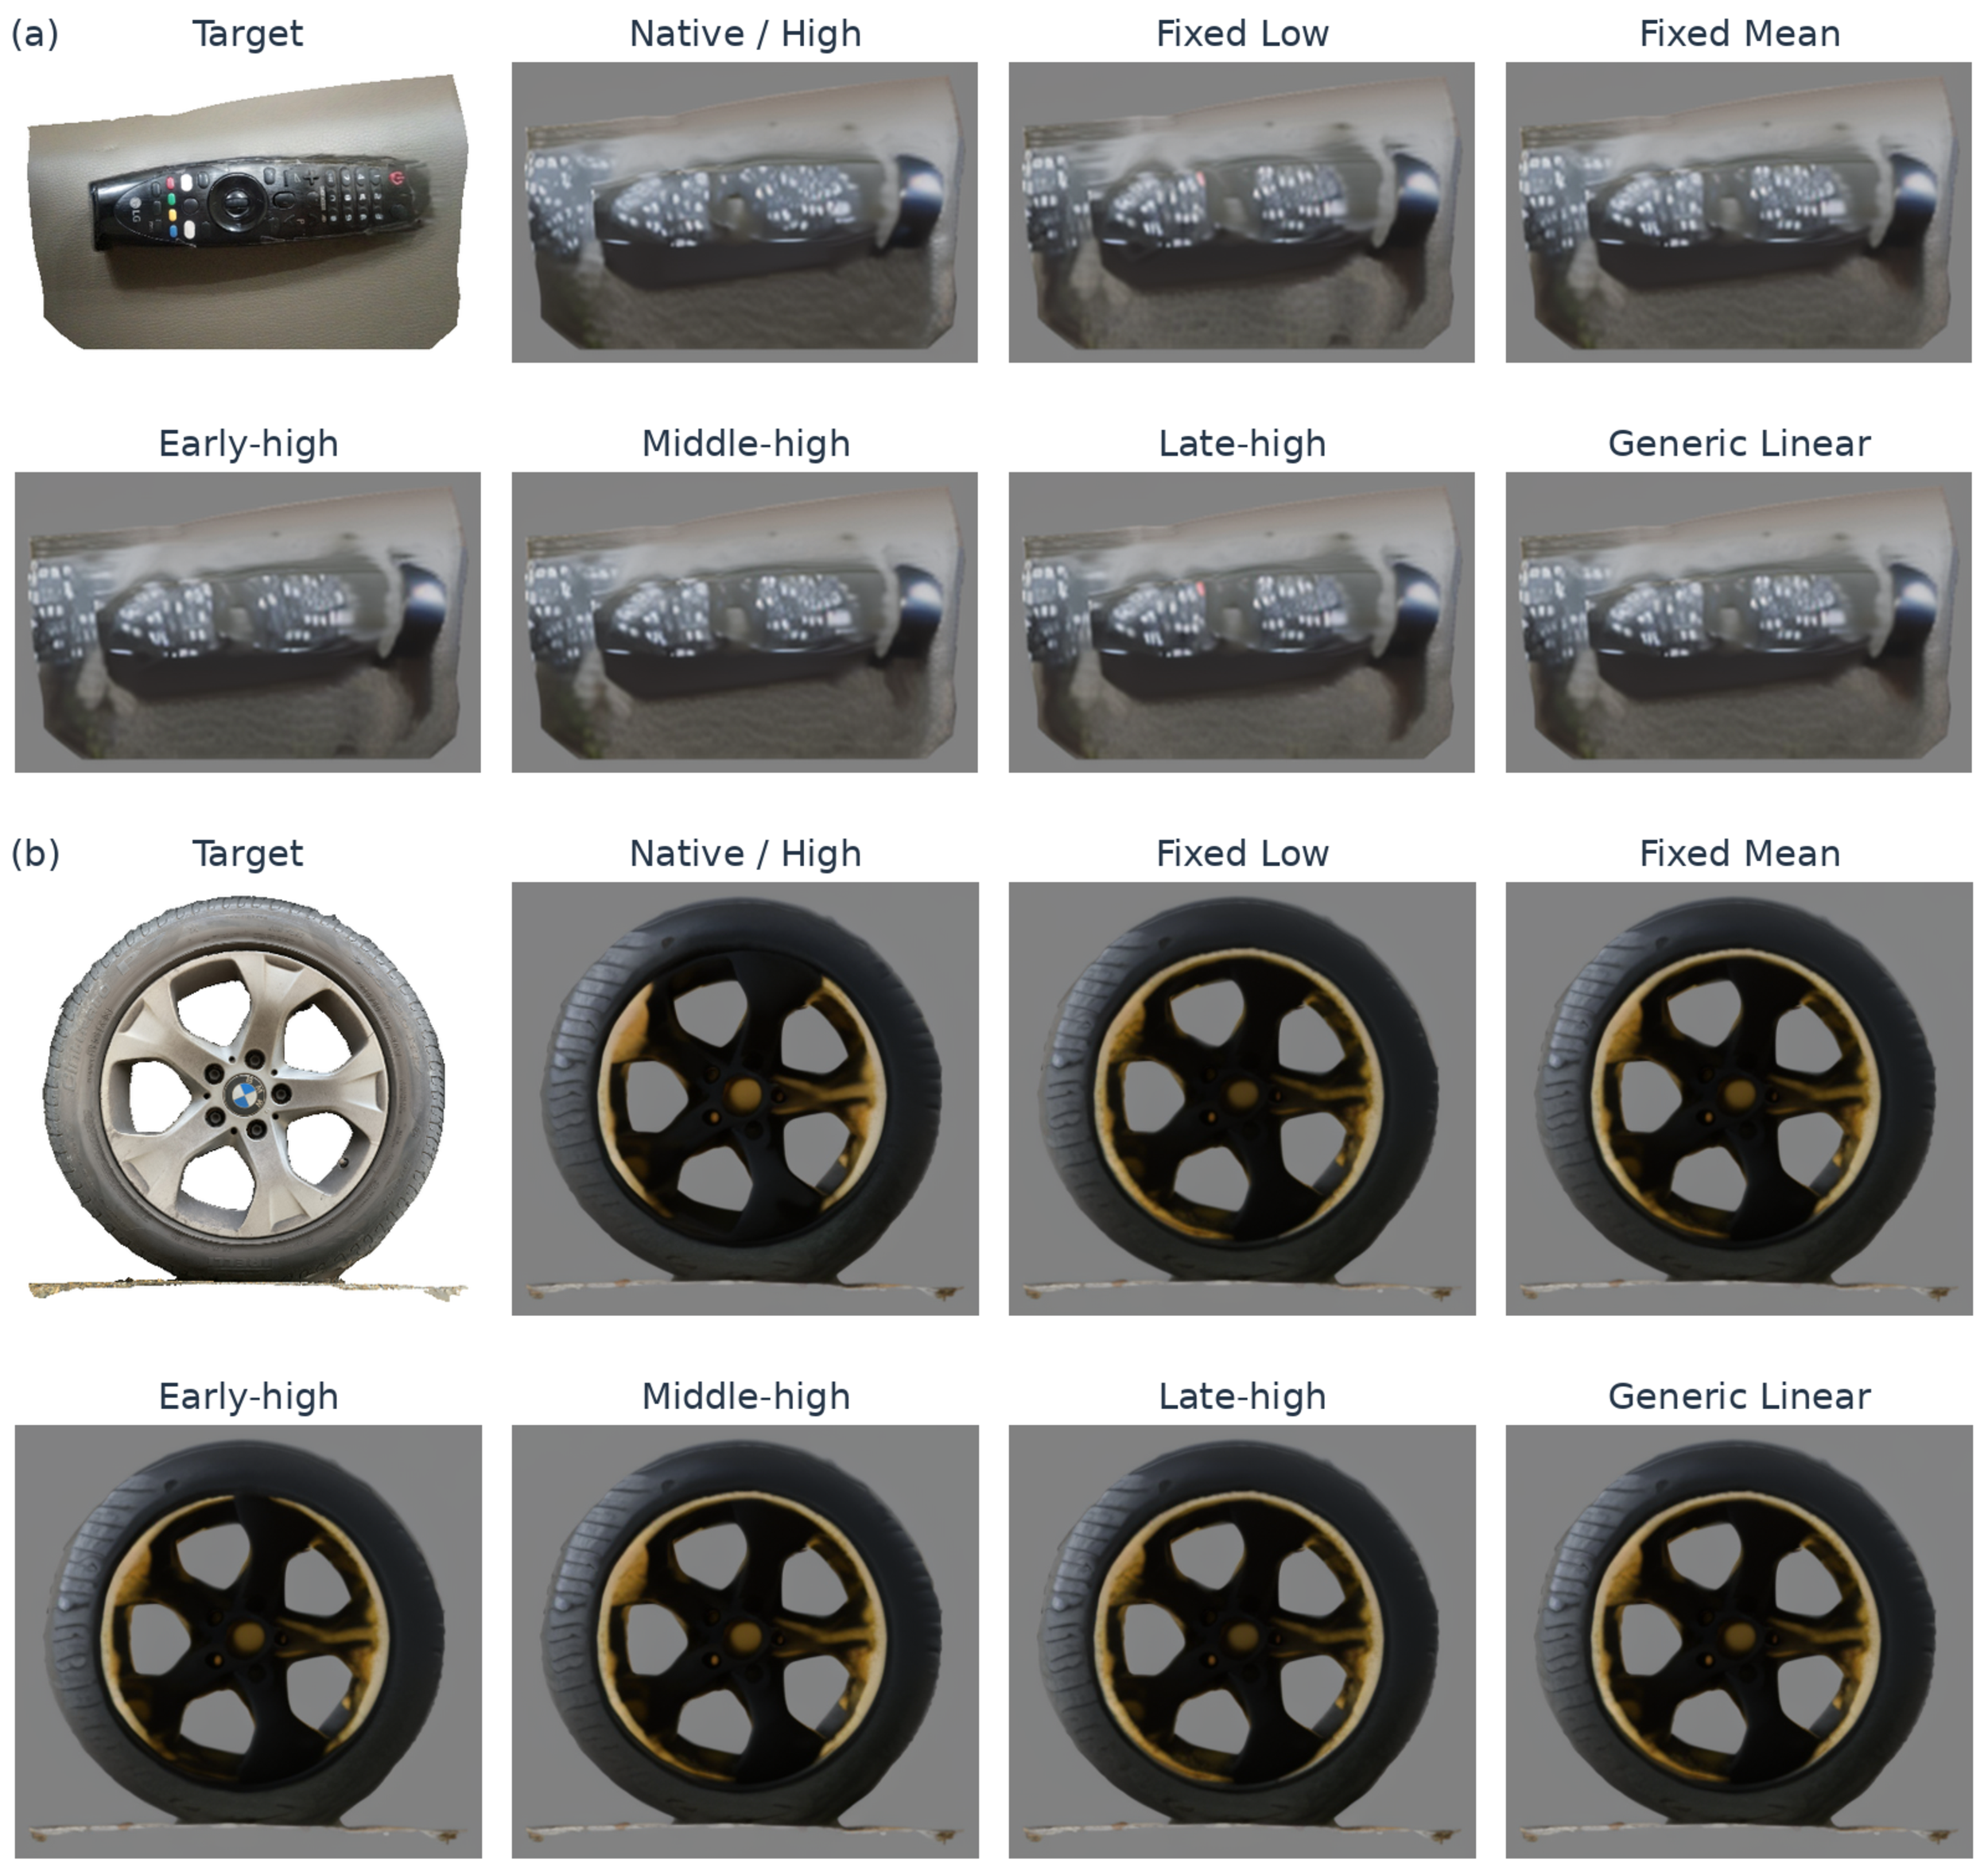
\includegraphics[width=\textwidth,height=0.72\textheight,keepaspectratio]{figures/figS_native50_all014.pdf}
\caption{Native MV-Adapter targets and all seven controls for the two examples discussed in the main text. All images use native view 0 and the same object seed; each object has one shared frame spanning target and every condition. Full asset attribution is in Supplementary Sections S5 and S9.}
\label{fig:supp-native50-full}
\end{figure}
\FloatBarrier
\section*{S4. GSO external-input and complete baked evaluation}
\label{supp:group4}
\addcontentsline{toc}{section}{S4. GSO external-input and complete baked evaluation}

\subsection*{Complete inherited-schedule extension and twenty-object bake}\label{supp:gso-complete}
\addcontentsline{toc}{subsection}{Complete inherited-schedule extension and twenty-object bake}
This extension uses the same source-selected GSO100 and native MV-Adapter interface. Four existing fixed/temporal/linear profiles were frozen before their outputs, after native/mean/late and auxiliary-correction results had been inspected. No new algorithm, model training or parameter search is involved. The main comparison follows the previous native50 question: middle-high minus fixed mean on all-six-view FG-PSNR, with three seeds averaged within object. The other 83 pair/metric endpoints use Holm83; the 21 nonreference LPIPS pairs use a separate exploratory Holm21 family. These families do not imply one overall experiment-wide error guarantee. The extension is external sensitivity, not pristine held-out confirmation.
\begin{table}[ht]\centering\small\begin{tabular}{lrrrr}\toprule Schedule & FG-PSNR & FG-LPIPS & FG-SSIM & $\Delta E_{00}$ \\\midrule
native & 16.998 & 0.11193 & 0.56736 & 12.550 \\
fixed low & 17.012 & 0.11316 & 0.56482 & 12.473 \\
fixed mean & 17.025 & 0.11239 & 0.56619 & 12.493 \\
early high & 16.974 & 0.11340 & 0.56414 & 12.538 \\
middle high & 17.012 & 0.11224 & 0.56563 & 12.483 \\
late high & 17.070 & 0.11228 & 0.56753 & 12.432 \\
generic linear & 17.045 & 0.11228 & 0.56687 & 12.462 \\
\bottomrule\end{tabular}\caption{GSO100 native-view schedule means, all six views within each object and three sampling seeds. Scale labels have interface-specific semantics.}\end{table}
The specified middle--mean primary difference is -0.013660 dB, with pointwise 95\% object interval [-0.030565,+0.003519] and paired sign-flip $p=0.122279$. Non-detection is not equivalence; complete secondary and nonreference contrasts are delivered.
\paragraph{Revised calibration and full twenty-object baking.}
The original discontinuous-UV-ramp gate failure is preserved. GT-only diagnostics on all twenty fixed inputs reproduce native masks and constant colors, and validate continuous nonlinear world-coordinate colors at the original mean/99th-percentile error bounds of 0.03/0.15. An independent two-island analytic fixture agrees to approximately $1.2\times10^{-7}$ and a deliberate image flip is detected. For the mouse and Hair Dryer, all high-error ramp texels on common diagnostic coverage have a flagged bilinear sampling footprint across a UV jump; errors decrease at higher diagnostic resolutions. This does not assert artifact-free seams: raw UV aliasing and unfilled coverage remain deployment limitations. The revised calibration is post hoc, after fifteen original object outcomes. Projection, masks, cameras, source/texture resolutions, material and geometry remain unchanged. All 375 original GLB hashes and metric records reproduce exactly. No object or method is discarded by quality direction.
The complete evaluation contains 740 unique bakes: twelve existing methods by3 seeds by20 objects plus20 GT self-bakes, with11 unseen cameras per bake. All foreground remains the reported quality region. Coverage is diagnostic; GT-bake error is not subtracted. The retained correction family uses its original Holm16, while the seven schedule-pair/four-metric diagnostic family uses Holm84.
\begin{table}[ht]\centering\scriptsize\begin{tabular}{lrrrr}\toprule Bake condition & FG-PSNR & FG-LPIPS & FG-SSIM & $\Delta E_{00}$ \\\midrule
GT reference bake & 19.364 & 0.06023 & 0.71369 & 5.105 \\
native & 15.479 & 0.10087 & 0.47814 & 12.031 \\
fixed mean & 15.500 & 0.10089 & 0.47847 & 11.973 \\
late high & 15.507 & 0.10098 & 0.47961 & 11.967 \\
grid projection & 15.149 & 0.10524 & 0.45925 & 12.323 \\
view projection & 14.998 & 0.10643 & 0.45467 & 12.502 \\
interaction projection & 15.163 & 0.10486 & 0.46112 & 12.247 \\
apg projection only & 15.500 & 0.10191 & 0.47829 & 11.952 \\
apg paper sd21 at native cfg & 15.305 & 0.10260 & 0.47667 & 12.474 \\
fixed low & 15.484 & 0.10109 & 0.47783 & 11.994 \\
early high & 15.479 & 0.10101 & 0.47697 & 11.998 \\
middle high & 15.473 & 0.10102 & 0.47757 & 12.033 \\
generic linear & 15.499 & 0.10099 & 0.47893 & 11.979 \\
\bottomrule\end{tabular}\caption{Full fixed20-object re-evaluation. Eleven views and sampling seeds are nested within object. Scanned color is not certified physical albedo or PBR.}\end{table}
Mean generated/nonreference versus unseen-baked method-rank Spearman correlation is 0.601399, with object-bootstrap 95\% interval [0.44020979020979023, 0.7332167832167833]. Rank agreement does not establish the same best method on every object.


The separately supplied \texttt{Supplementary\_GSO\_Baked\_Comparison.mp4} shows the first source-ordered object, \texttt{Razer\_Abyssus\_Ambidextrous\_Gaming\_Mouse}, at seed 42, with all twelve recorded conditions and eleven actual unseen cameras (protocol indices 0--10). Each camera is held for 0.5 seconds. Its first column is an original source-mesh render, not the matched GT self-bake; the latter is assessed separately in the table above. The video is illustrative and does not estimate prevalence or material fidelity.

The specified Late-high minus Fixed Mean unseen-view FG-LPIPS difference is +0.00008379, with pointwise 95\% object interval [-0.00010305,+0.00028592] and original Holm16 adjusted $p=0.78765$. This study does not detect the ten-object GeoTex pilot's benefit; it uses a different domain and interface/projection protocol.

\paragraph{Post hoc sensitivity of image/bake rank agreement.}
The all-twelve-method estimate includes auxiliary corrections that differ markedly in quality. Restricting the same twenty objects to native, fixed low, fixed mean, early-high, middle-high, late-high and generic linear gives mean within-object Spearman 0.396429, with pointwise object-bootstrap 95\% interval [0.175000,0.582143] (20,000 resamples, seed 131313). The minimum-mean LPIPS condition changes on 11/20 objects. This is a post hoc descriptive analysis, retaining every object. It changes neither the primary endpoint nor the original adjusted families; point-estimate winner changes do not establish statistically resolved best methods. Raw pairs and a portable recomputation are delivered in data/FACTS\_round\_014.json and scripts/build\_evidence.py.

\subsection*{Separate projection/APG comparison and archived original bake failure}
\addcontentsline{toc}{subsection}{Separate projection/APG comparison and archived original bake failure}
\paragraph{Completed GSO100 external comparison.}
The source-selected canonical GSO100 inputs have matched native-camera reference view 1 and six target views. The six-condition, three-seed matrix contains 1,800 generated cells, followed by 600 cells for two separately frozen APG baselines. The main LPIPS endpoint excludes reference view 1; seeds are averaged within each of the 100 objects. Native/default identity and native-camera target checks pass. These scanned-color textures are not certified physical albedo or PBR ground truth.

\begin{table}[ht]\centering\small
\begin{tabular}{llrr}
\toprule
Correction & Baseline & LPIPS difference & Holm $p$ \\
\midrule
grid projection & native & $+0.012381$ & $4.5e-05$ \\
grid projection & fixed mean & $+0.011581$ & $4.5e-05$ \\
grid projection & late high & $+0.011667$ & $4.5e-05$ \\
view projection & native & $+0.014637$ & $4.5e-05$ \\
view projection & fixed mean & $+0.013836$ & $4.5e-05$ \\
view projection & late high & $+0.013923$ & $4.5e-05$ \\
interaction projection & native & $+0.011174$ & $4.5e-05$ \\
interaction projection & fixed mean & $+0.010374$ & $4.5e-05$ \\
interaction projection & late high & $+0.010460$ & $4.5e-05$ \\
grid projection & apg projection only & $+0.009113$ & $3e-05$ \\
grid projection & apg paper sd21 at native cfg & $+0.008553$ & $3e-05$ \\
view projection & apg projection only & $+0.011369$ & $3e-05$ \\
view projection & apg paper sd21 at native cfg & $+0.010809$ & $3e-05$ \\
interaction projection & apg projection only & $+0.007906$ & $3e-05$ \\
interaction projection & apg paper sd21 at native cfg & $+0.007347$ & $3e-05$ \\
\bottomrule\end{tabular}
\caption{All specified GSO100 primary correction-minus-baseline contrasts. LPIPS is lower-better; every positive difference favors the baseline. Holm9 applies to the nine scale-control comparisons and Holm6 to the six APG comparisons, as separate frozen families. Complete pointwise intervals and secondary metrics are delivered.}
\end{table}

All fifteen primary correction comparisons favor the baselines; the three seed means have the same direction. Relative to native, grid, view and interaction correction are worse on 93, 91 and 88 of 100 object means, respectively. The APG SD2.1 clipping/momentum setting uses native CFG 3, not the original paper's CFG 10. The APG protocol was frozen before its outputs but after candidate generation had begun; this is not a joint preregistration. An independent object/seed table reconstruction matches all reported paired means.

\paragraph{Original calibration failure and complete fixed-cohort reevaluation.}
The fixed twenty-object native-UV sequence shares eight methods, three seeds and eleven unseen views. Rank 0 completes ten objects and rank 1 completes five, for 375 rows including fifteen GT self-bakes. Before candidate quality evaluation on \texttt{Remington\_\allowbreak TStudio\_\allowbreak Hair\_\allowbreak Dryer}, its UV-ramp calibration gives mean error 0.007023 (below 0.03) but 99th-percentile error 0.178684 (above the frozen 0.15). Native-camera masks and constant-color calibration pass. The original supervisor and delivery stop on that failure. A documented GT-only calibration addendum subsequently completes all twenty fixed inputs, including four inherited schedule controls, for 740 unique bakes and 8,140 unseen-view rows. All 375 earlier GLB hashes and metric records reproduce exactly. The full results, raw failure and revised-calibration scope are reported above in this section. The completed rows and failed gate remain archived; no unfavorable object is removed to obtain a method advantage.

\FloatBarrier
\subsection*{Fixed-seed stability: complete descriptive addendum}
\addcontentsline{toc}{subsection}{Fixed-seed stability: complete descriptive addendum}
This analysis was proposed after inspection of the completed GSO results. Each seed-specific value averages the appropriate views within object. Its pointwise 95\% interval resamples objects (20,000 draws; seed 20261012). All three fixed seeds and all four named rows are retained; seeds are not additional independent objects. The all-six-view image primaries, five-nonreference-view LPIPS and eleven-unseen-view bake remain distinct. Direction agreement uses zero only and is not a meaningful-effect or non-inferiority threshold. We define no new confirmatory test or significance family for these descriptive intervals.

\begin{table}[ht]\centering\scriptsize\setlength{\tabcolsep}{3pt}
\caption{Fixed-seed conditional mean A minus B and number of objects with favorable/adverse directions at all three seeds. Higher favors PSNR; lower favors LPIPS. The remaining objects have mixed or tied directions.}\label{tab:seed-stability015}
\begin{tabular}{lrrrrr}\toprule Contrast / endpoint & 42 & 2026 & 31415 & All favorable & All adverse \\
\midruleGSO100 Middle--Mean PSNR & -0.00835 & -0.02374 & -0.00889 & 14/100 & 24/100 \\
GSO100 Late--Mean PSNR & +0.05675 & +0.03832 & +0.03868 & 27/100 & 5/100 \\
GSO100 Late--Mean nonreference LPIPS & -0.000389 & -0.000269 & +0.000398 & 24/100 & 14/100 \\
GSO20 Late--Mean unseen LPIPS & -0.000064 & +0.000308 & +0.000007 & 1/20 & 5/20 \\
\bottomrule\end{tabular}
\end{table}
\begin{figure}[ht]\centering
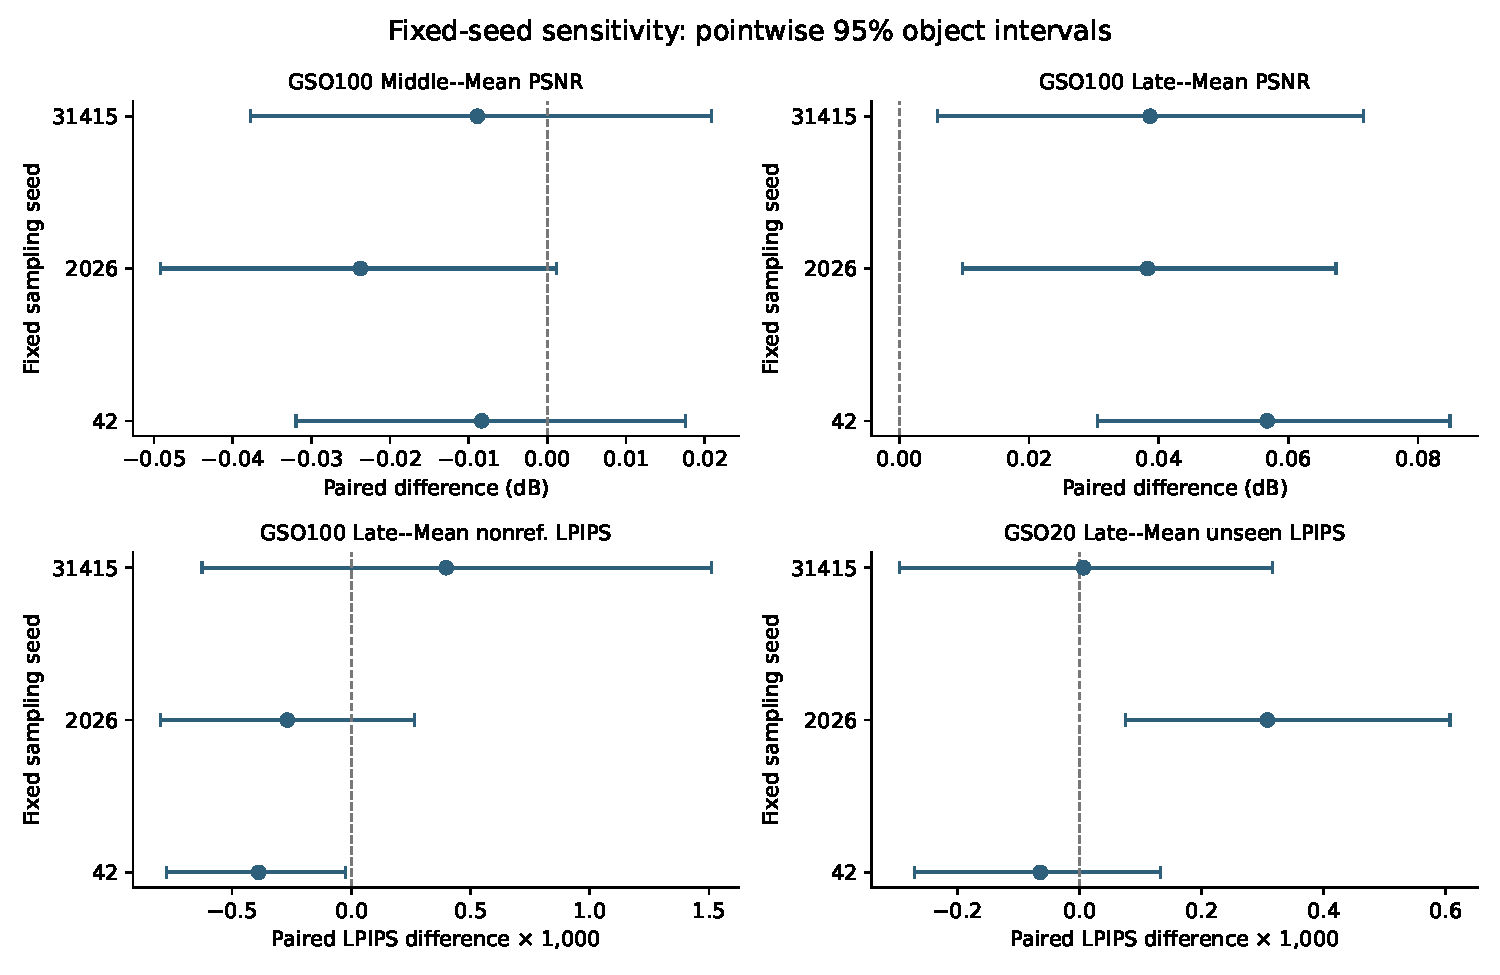
\includegraphics[width=.95\textwidth]{figures/fig_seed_stability015.pdf}
\caption{Seed-specific paired means with pointwise object intervals. Three fixed seeds do not estimate the complete distribution of inference or training randomness. The original seed-averaged tests remain unchanged.}\label{fig:seed-stability015}
\end{figure}
For Late--Mean PSNR, all three cohort means are positive, yet 68/100 objects have mixed/tied signs. For nonreference LPIPS, the third seed reverses the cohort-average direction. In GSO20, one object has favorable LPIPS at all seeds, five adverse at all seeds and fourteen mixed/tied. Small average effects therefore provide limited assurance of repeatable per-object improvement. Complete per-object seed deltas and descriptive intervals are supplied in the data addendum; no seed or object is removed for its outcome.

\FloatBarrier
\section*{S5. Calibrated GeoTex baked appearance and earlier attempts}
\label{supp:group5}
\addcontentsline{toc}{section}{S5. Calibrated GeoTex baked appearance and earlier attempts}

\subsection*{Calibrated bake pilot, historical separation and actual-output displays}\label{supp:bake10-complete}
\addcontentsline{toc}{subsection}{Calibrated bake pilot, historical separation and actual-output displays}
\paragraph{Projection protocol and superseded attempts.}
The earlier five-object bake rotated generated pole-view RGB back into raw-camera coordinates but also incorrectly rotated the raw-camera mask. Four of five objects have affected masks. Its old quality estimates are superseded by corrected evaluation and are not pooled with newly selected objects. In the REPEAT branch, bilinear fractions must be calculated before wrapping integer indices: the previous order could produce negative weights at tile edges and outside [0,1]. Corrected code passes nonnegative/unit-sum weight checks and integer-period translation invariance. Scalar coverage masks are read without an RGB transfer function; decoding grayscale coverage as sRGB would change the foreground threshold. GT source images are resized to 256 using bicubic RGB and the same nearest-index alpha masks as generated sources; atlas, camera, fill and render parameters are shared. The original GT-512 bake is retained only as an unmatched-resolution diagnostic.

The ten-object bake pilot uses objects chosen in frozen UID order before observing their bake results. All 300 Fresh C inputs were screened; old five-object outputs and the previously inspected REPEAT diagnostic object were excluded. Eligibility required available source GLB, one opaque white-factor base-color material, native TEXCOORD\_0, no vertex colors, at most 300,000 triangles, and source camera-mask alignment passing the frozen gate. This input-selected set is smaller than the target twenty and below fifteen; we retain the pilot designation and all ten outcomes. No failed or adverse-quality object was replaced. Seven conditions generated 70 object-condition rows; eight bake conditions including GT generated 80 artifacts, with 880 unseen renders and 480 source-camera renders.

The frozen primary was Late-high--Fixed Mean FG-LPIPS. C3--GFH PSNR, LPIPS, SSIM and CIEDE2000 form one four-test secondary Holm family. All other complete pairs are descriptive. Views are averaged before inference. Intervals use 50,000 paired object resamples and are pointwise, not simultaneous. The ten-object primary uses all $2^{10}$ sign flips; the secondary family uses the same exact test. A sign-flip test assumes symmetry/exchangeability of paired differences under its null; an interval alone is not a practical-equivalence criterion. No non-inferiority margin was chosen.

\begin{table}[ht]\centering\scriptsize
\caption{Prespecified new-pilot comparisons: raw A minus B, 95\% object-bootstrap interval; no pooling with old five.}\label{tab:bake-paired}
\begin{tabular}{llrr}
\toprule Contrast & Endpoint & Mean [95\% CI] & $p$ \\
\midrule
Late--Mean & FG-LPIPS & $-0.00265\ [-0.00414,-0.00137]$ & 0.00195 (primary) \\
C3--GFH & FG-PSNR & $+0.193\ [-0.649,+0.875]$ & 1.000 (Holm) \\
C3--GFH & FG-LPIPS & $-0.00036\ [-0.00396,+0.00336]$ & 1.000 (Holm) \\
C3--GFH & FG-SSIM & $-0.05274\ [-0.07459,-0.03170]$ & 0.00781 (Holm) \\
C3--GFH & CIEDE2000 & $-1.102\ [-2.915,+0.939]$ & 0.95508 (Holm) \\
\bottomrule\end{tabular}\end{table}

The corrected earlier five-object bake uses the same source-resolution and mask corrections but retains its historical clamped-UV technical scope. Its descriptive means (PSNR / LPIPS / SSIM) are GFH 11.86 / 0.1609 / 0.5513, C3 14.24 / 0.1542 / 0.4170, Fixed Mean 14.19 / 0.1538 / 0.4348 and Late-high 15.02 / 0.1479 / 0.4428. C3--GFH is $+2.37$ dB, not the superseded $+2.27$ dB estimate. There was no independent predeclared primary for this reevaluation. The older N=20 result, old five, new ten and corrected single-object REPEAT diagnostic each retain separate source identifiers. Earlier wrong-mask, gamma-decoded-alpha and wrong-REPEAT-weight artifacts remain audit records and are superseded, never combined with the valid reevaluation.

\begin{table}[ht]\centering\scriptsize
\caption{Per-object generated-view versus unseen-bake rankings across seven conditions. Bootstrap unit is object. Positive overall agreement does not require an identical winning condition.}
\begin{tabular}{lrr}
\toprule Endpoint & Mean Spearman $\rho$ [95\% CI] & Winner changed \\
\midrule
FG-PSNR & $0.846\ [0.696,0.968]$ & 1/10 \\
FG-LPIPS & $0.804\ [0.693,0.911]$ & 7/10 \\
FG-SSIM & $0.746\ [0.450,0.964]$ & 4/10 \\
Edge-SSIM & $0.907\ [0.871,0.943]$ & 6/10 \\
\bottomrule\end{tabular}\end{table}

GT and generated bake sources use the same six raw cameras and 256-pixel resolution. GT RGB uses bicubic downsampling; alpha uses the exact nearest-index mapping used for generated foreground inputs. Their six-view scalar masks are bitwise identical and their raw atlas coverage matches for every object and condition. No unseen view enters baking. Export checks retain binary geometry/UV buffers, transforms and mesh identity. REPEAT UV weights are nonnegative, sum to one and are invariant under integer UV shifts. These checks establish a valid unlit projection comparison, not PBR equivalence or a validated seam score. Texture boundaries can be natural appearance boundaries; seam diagnostics are not reported as a validated primary endpoint.

The seven rights-cleared galleries below show matched source, GT-256 and generated bakes at unseen camera 004, using a shared whole-object frame. Visible failures are retained. The full ten-object pilot remains in the numerical analysis, including the three objects without verified display rights; these seven displays do not estimate cohort prevalence.

\begin{figure}[p]\centering
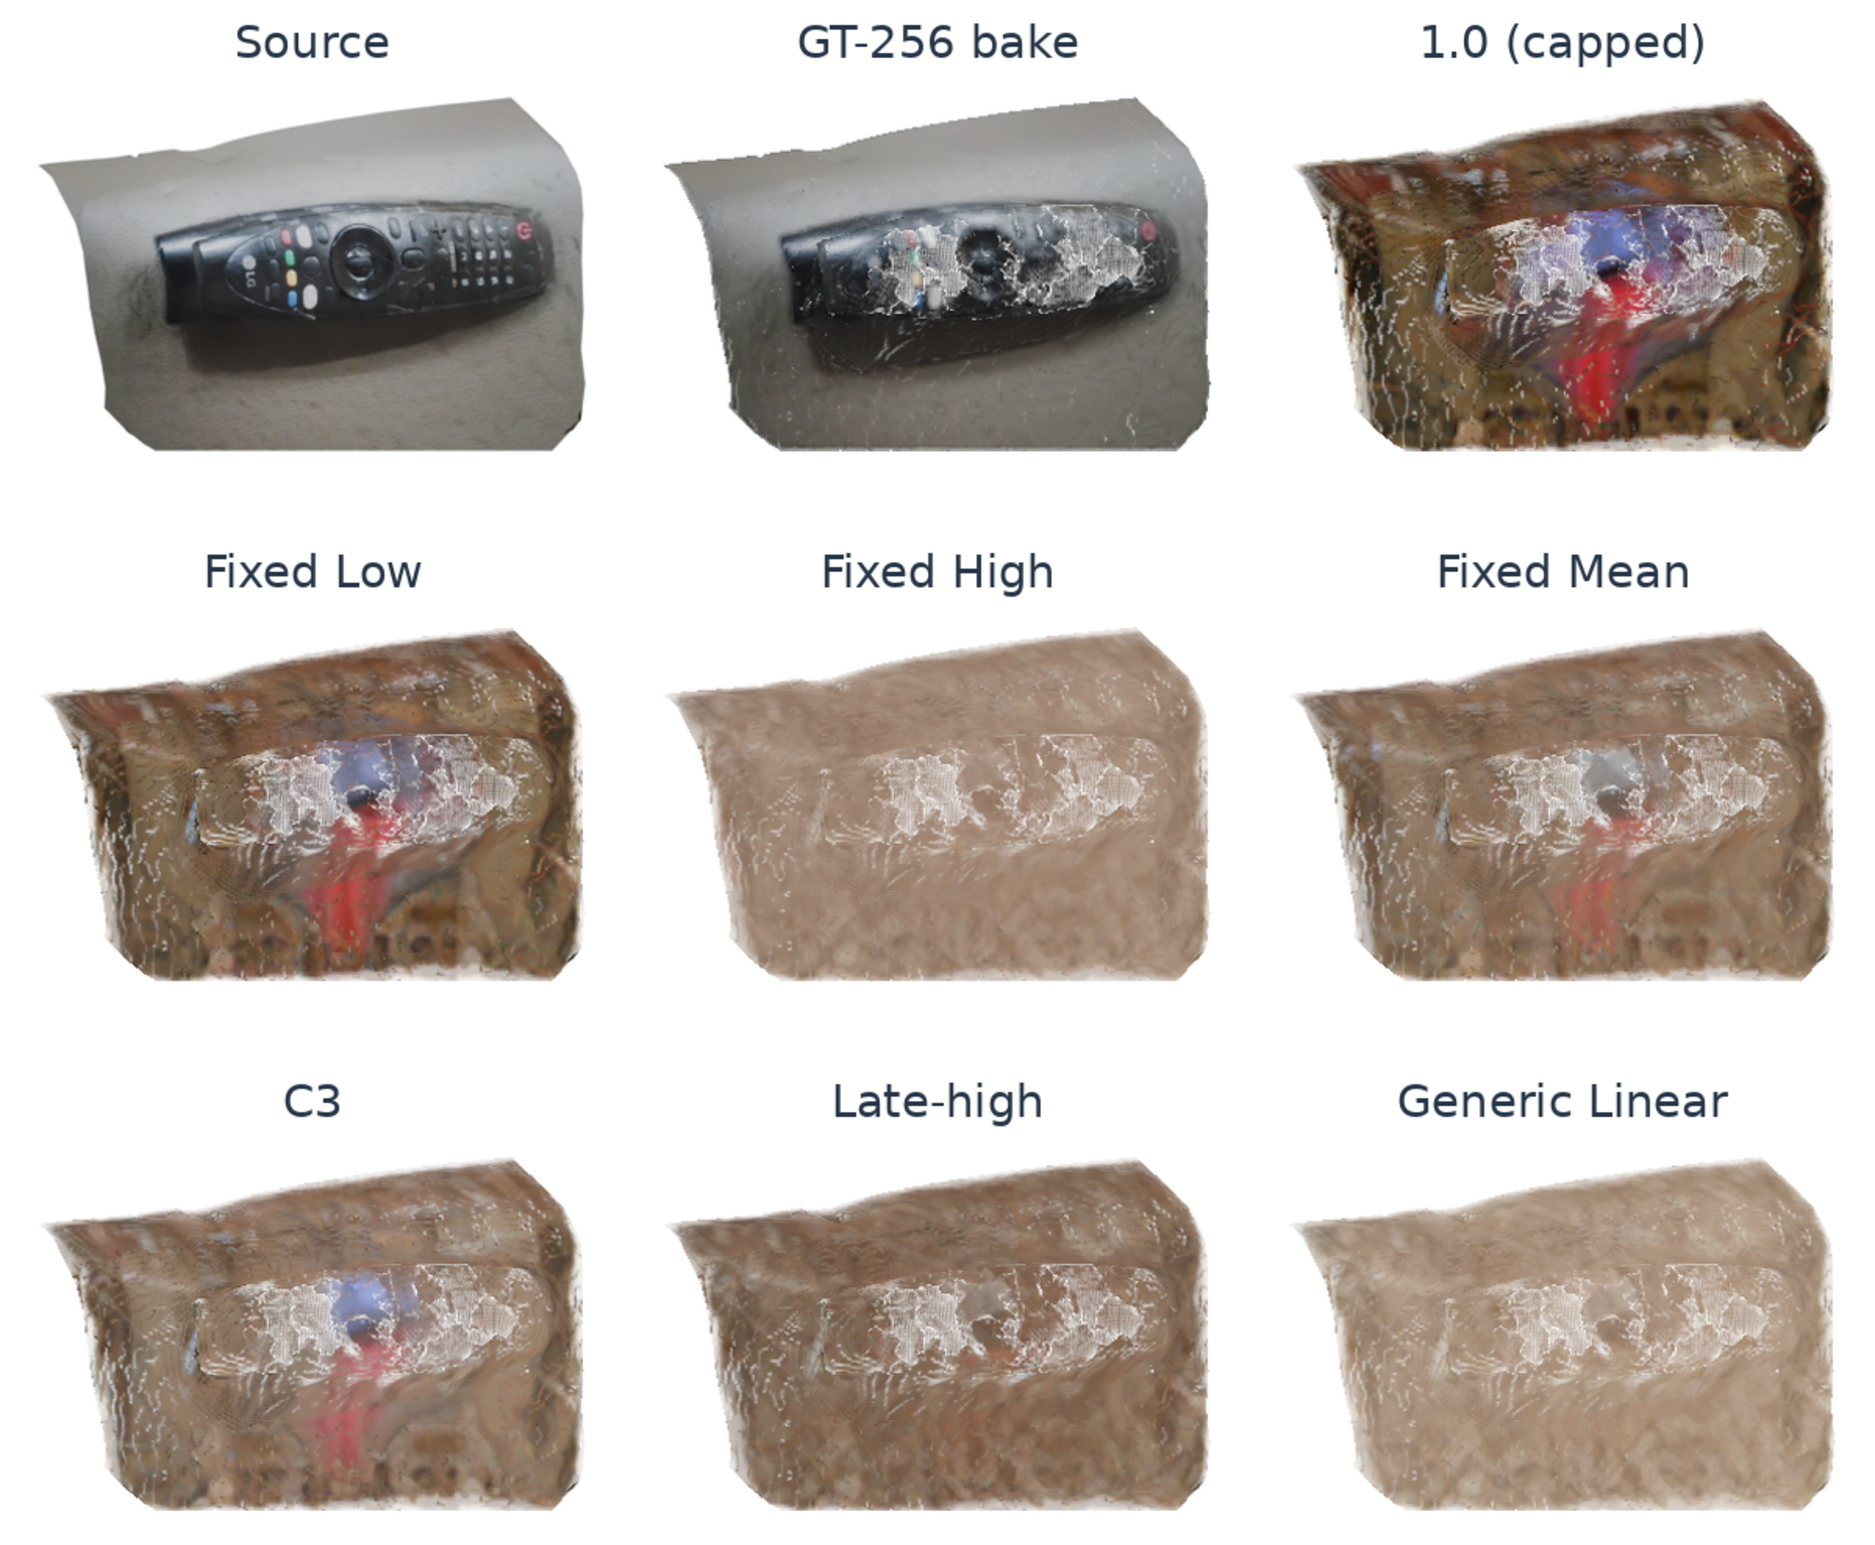
\includegraphics[width=\textwidth,height=0.72\textheight,keepaspectratio]{figures/figS_bake014_01.pdf}
\caption{Rights-cleared GeoTex bake display 1 of seven at unseen camera 004. Source, matched GT-256 reference bake and all seven generated conditions share one whole-object frame.}
\end{figure}

\begin{figure}[p]\centering
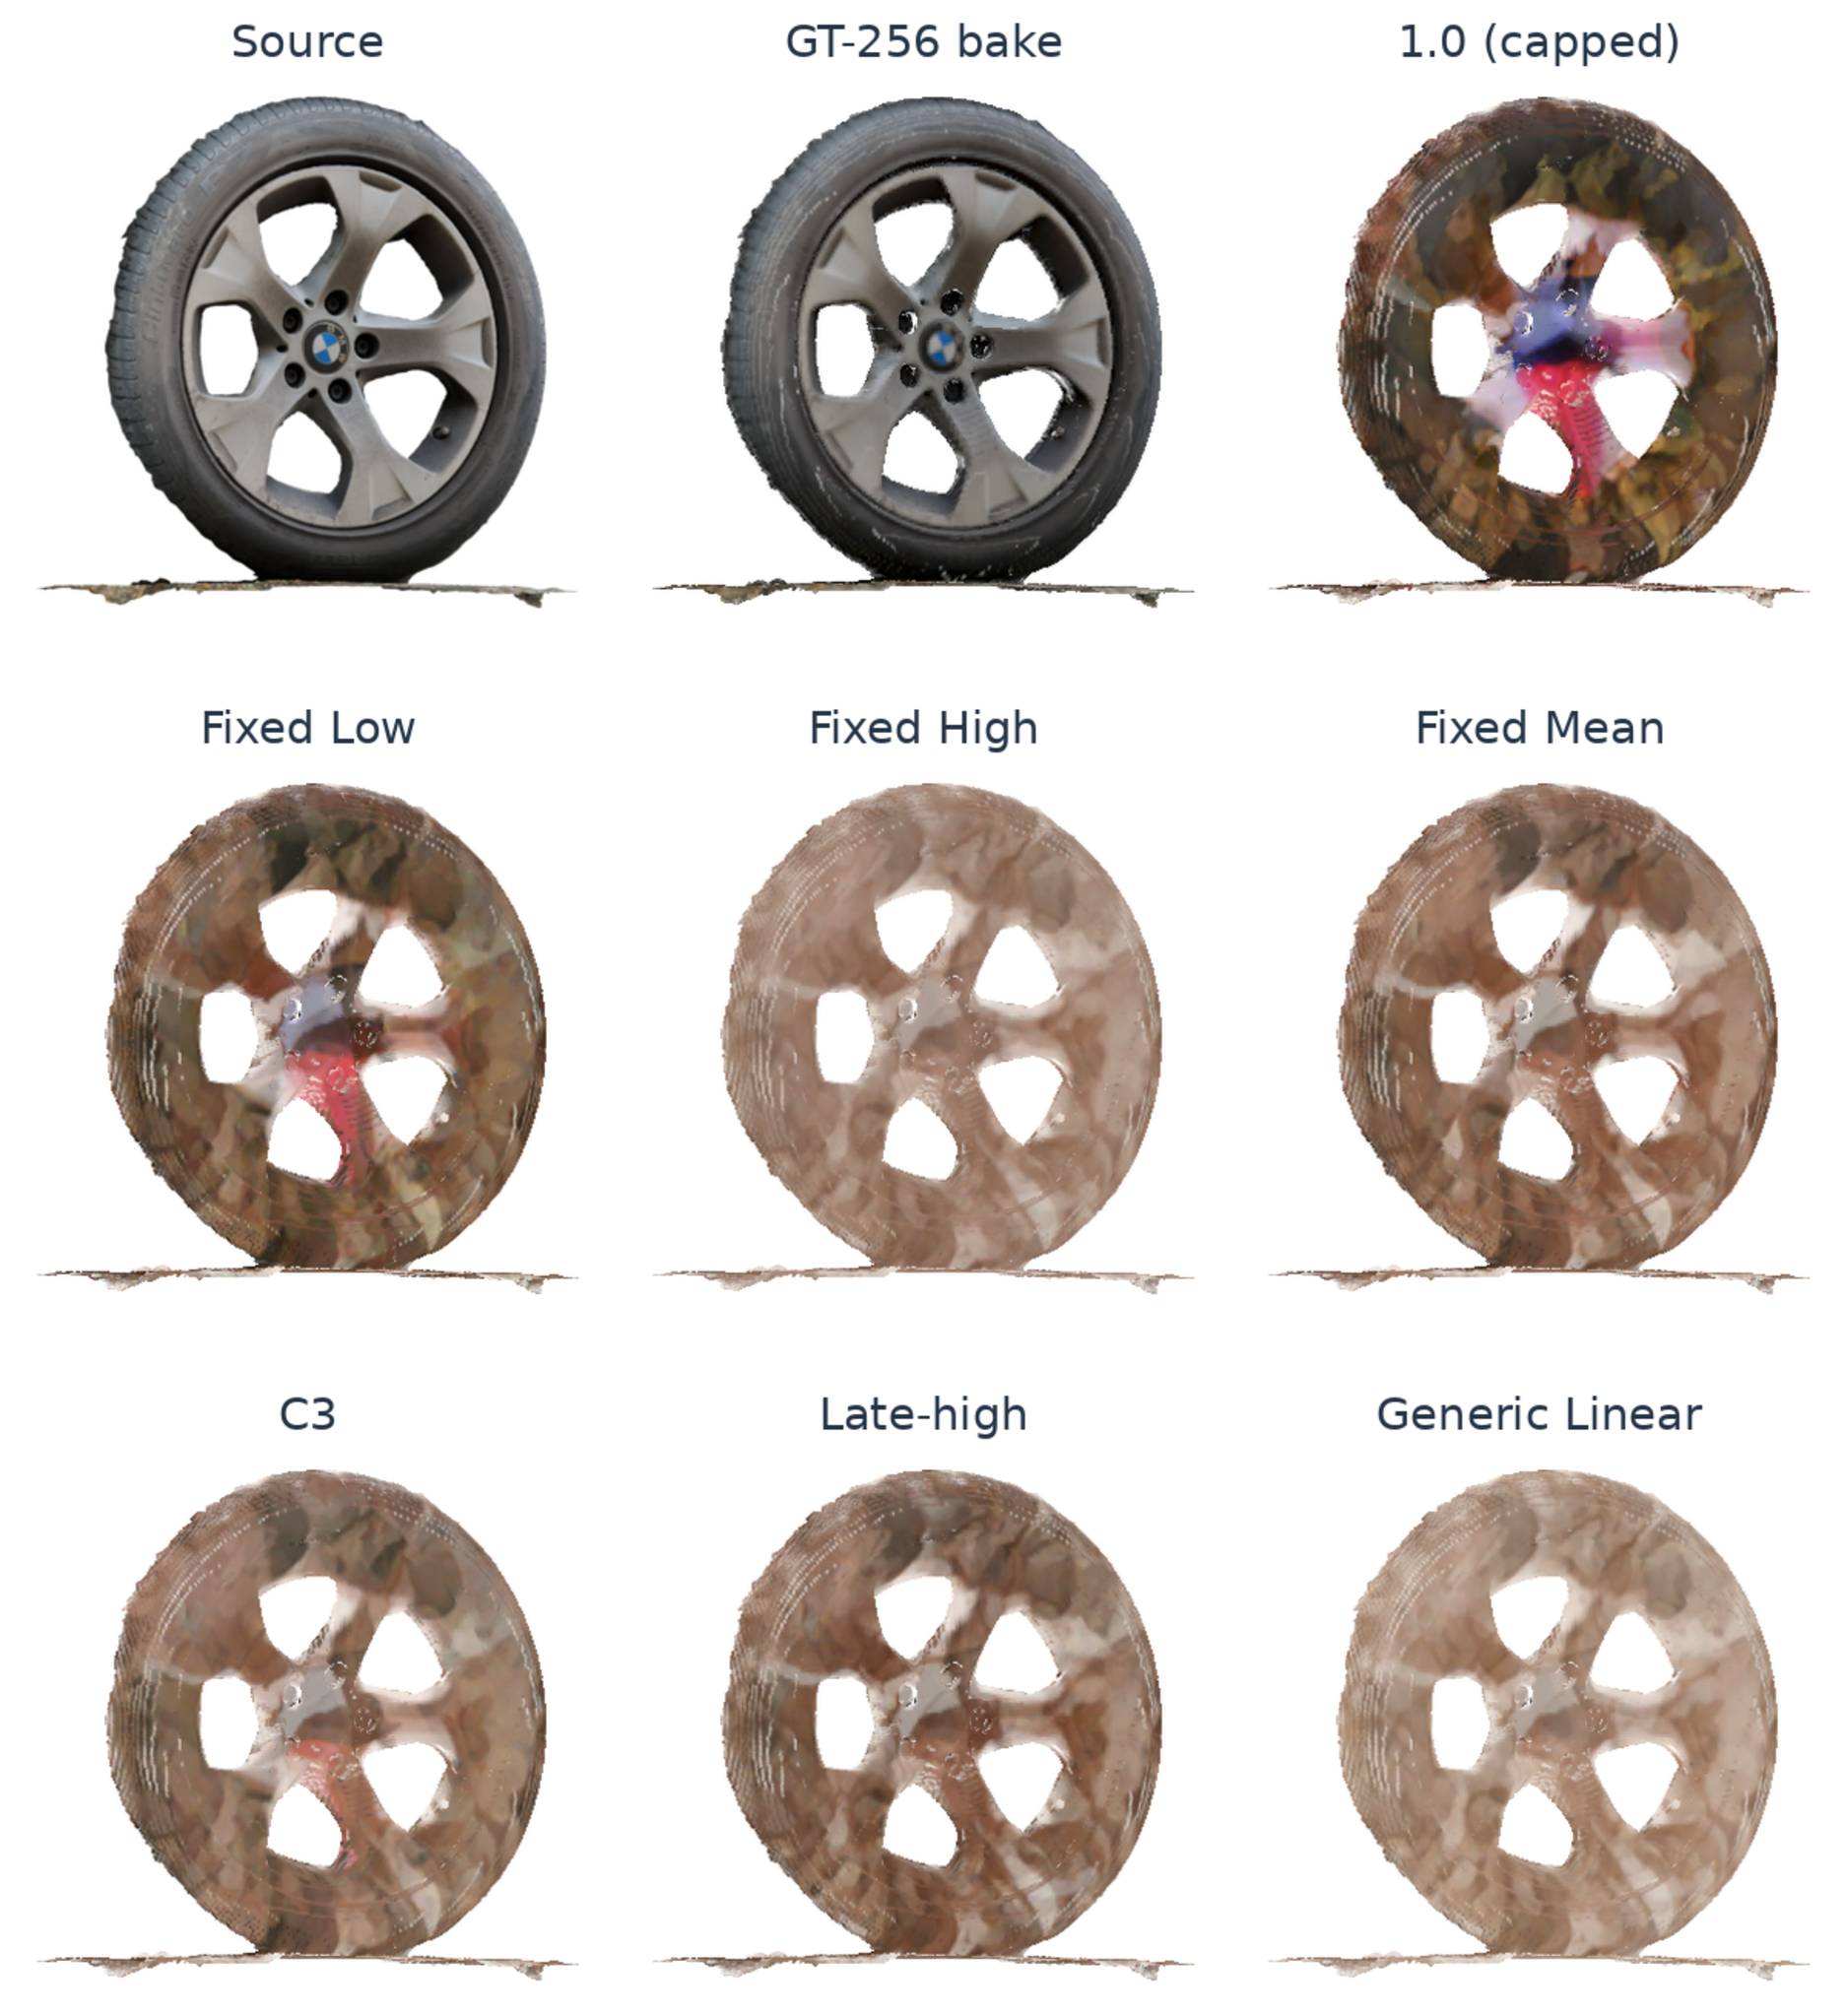
\includegraphics[width=\textwidth,height=0.72\textheight,keepaspectratio]{figures/figS_bake014_02.pdf}
\caption{Rights-cleared GeoTex bake display 2 of seven at unseen camera 004. Source, matched GT-256 reference bake and all seven generated conditions share one whole-object frame.}
\end{figure}

\begin{figure}[p]\centering
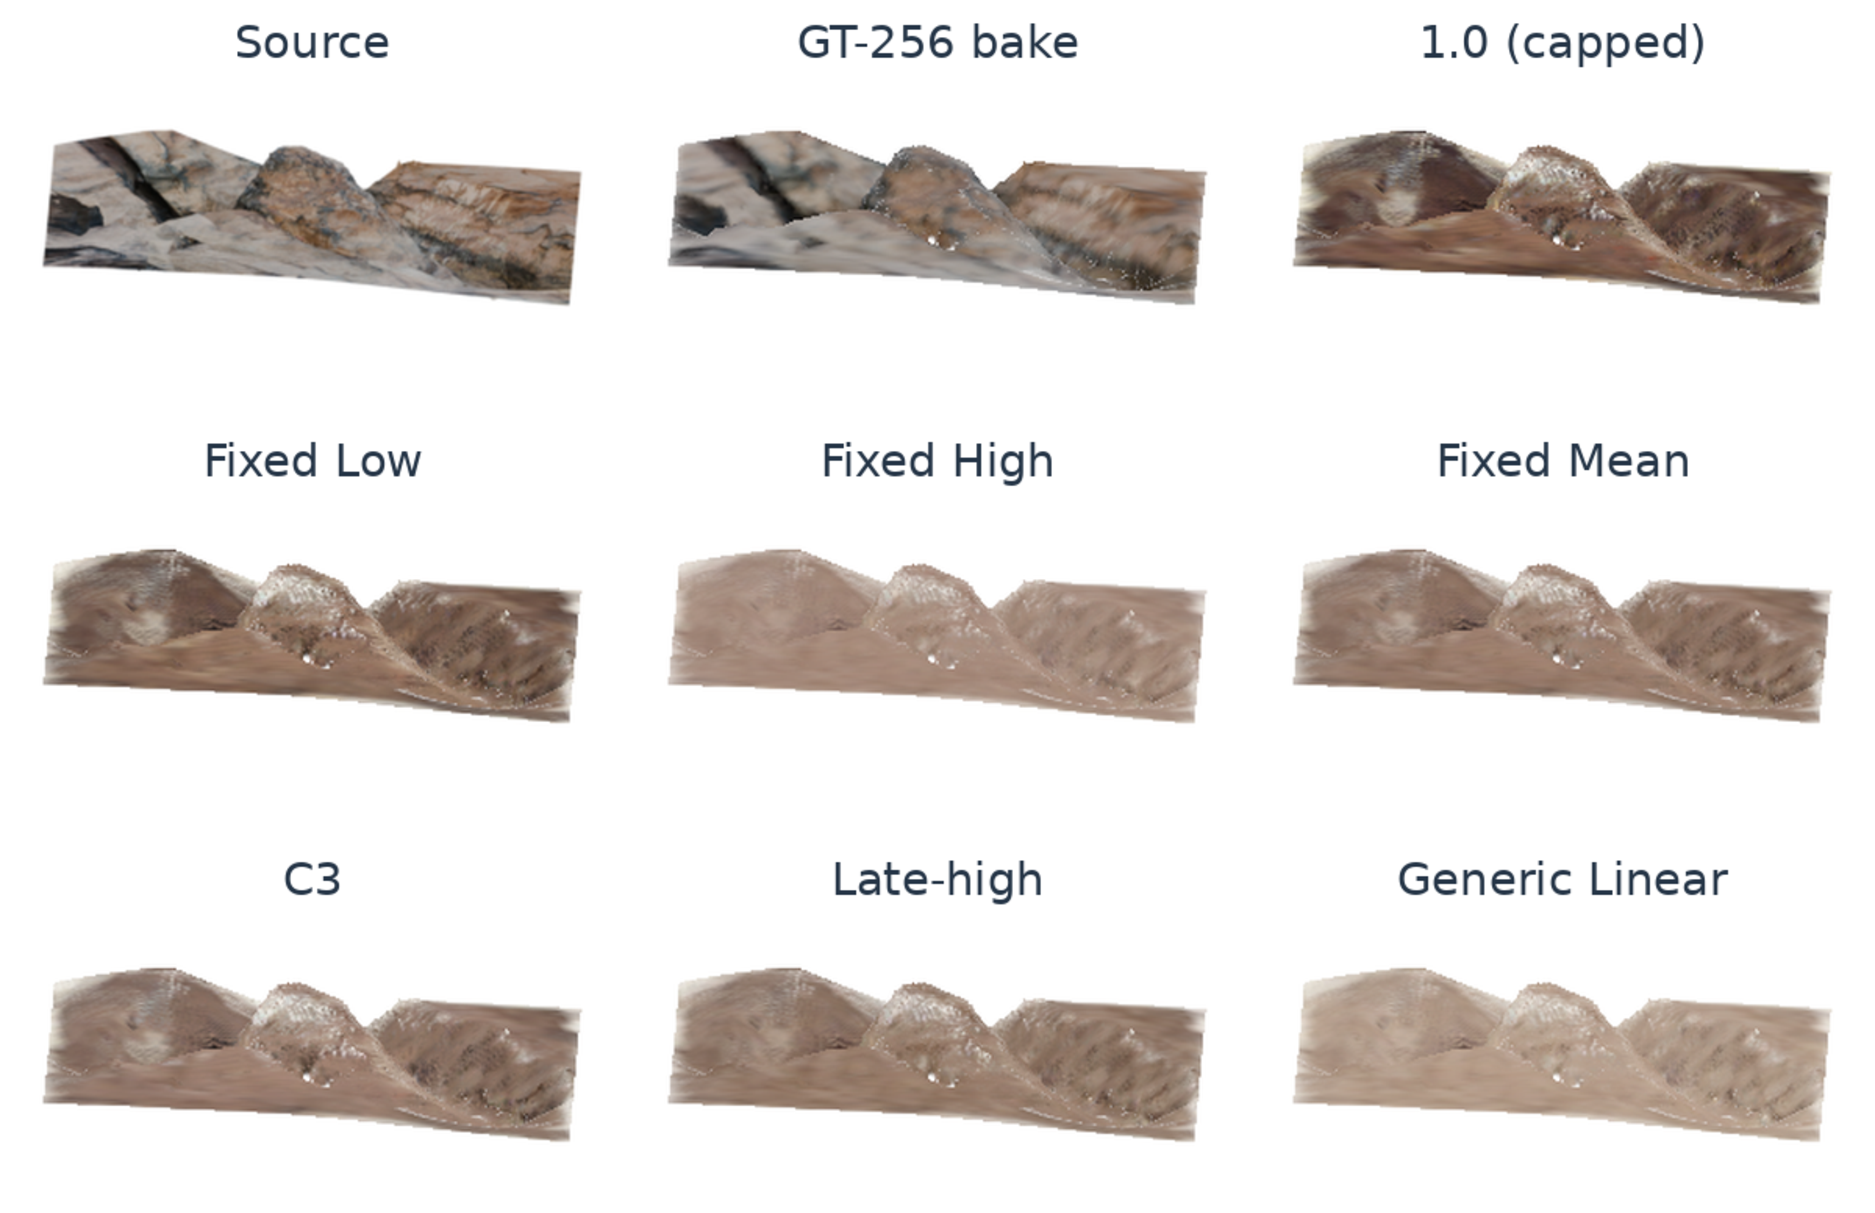
\includegraphics[width=\textwidth,height=0.72\textheight,keepaspectratio]{figures/figS_bake014_03.pdf}
\caption{Rights-cleared GeoTex bake display 3 of seven at unseen camera 004. Source, matched GT-256 reference bake and all seven generated conditions share one whole-object frame.}
\end{figure}

\begin{figure}[p]\centering
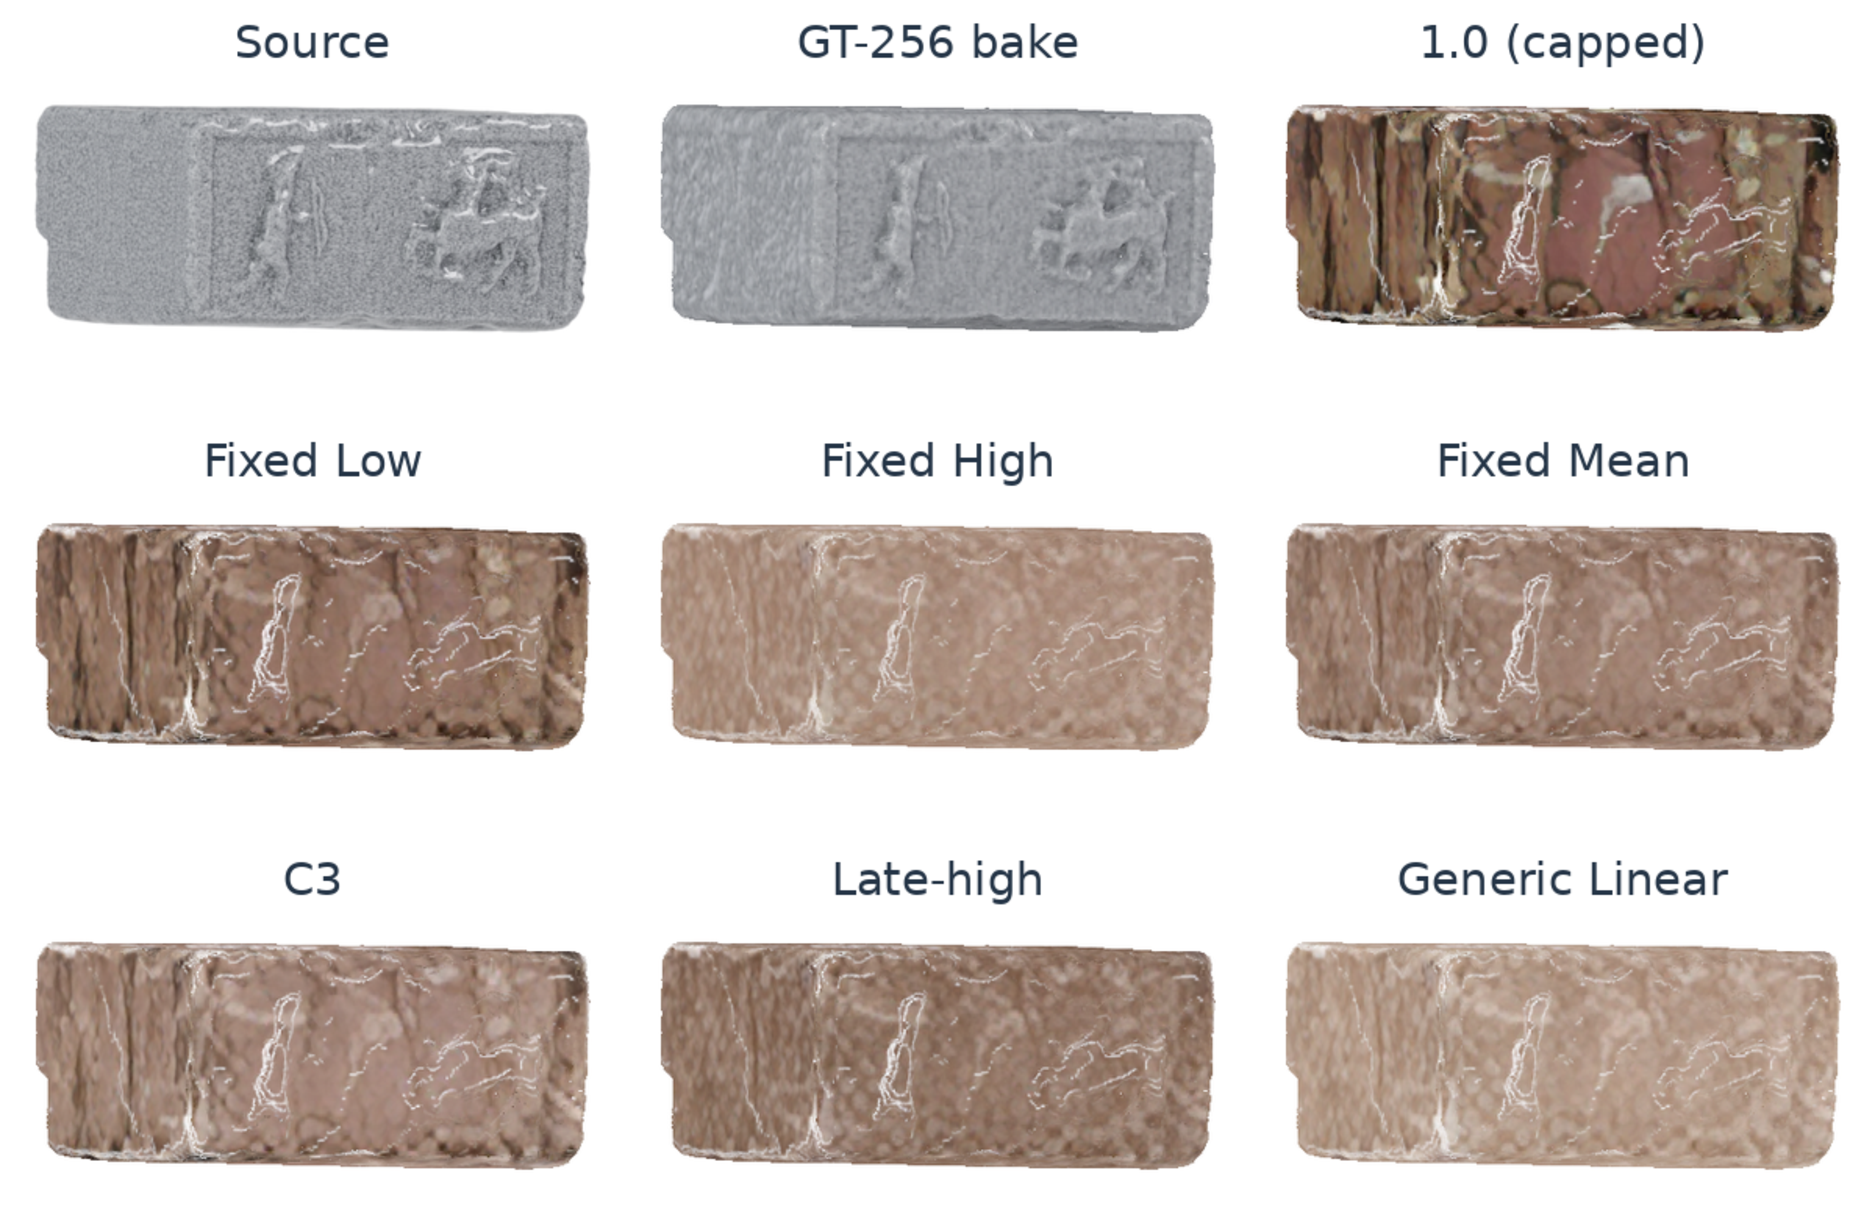
\includegraphics[width=\textwidth,height=0.72\textheight,keepaspectratio]{figures/figS_bake014_04.pdf}
\caption{Rights-cleared GeoTex bake display 4 of seven at unseen camera 004. Source, matched GT-256 reference bake and all seven generated conditions share one whole-object frame.}
\end{figure}

\begin{figure}[p]\centering
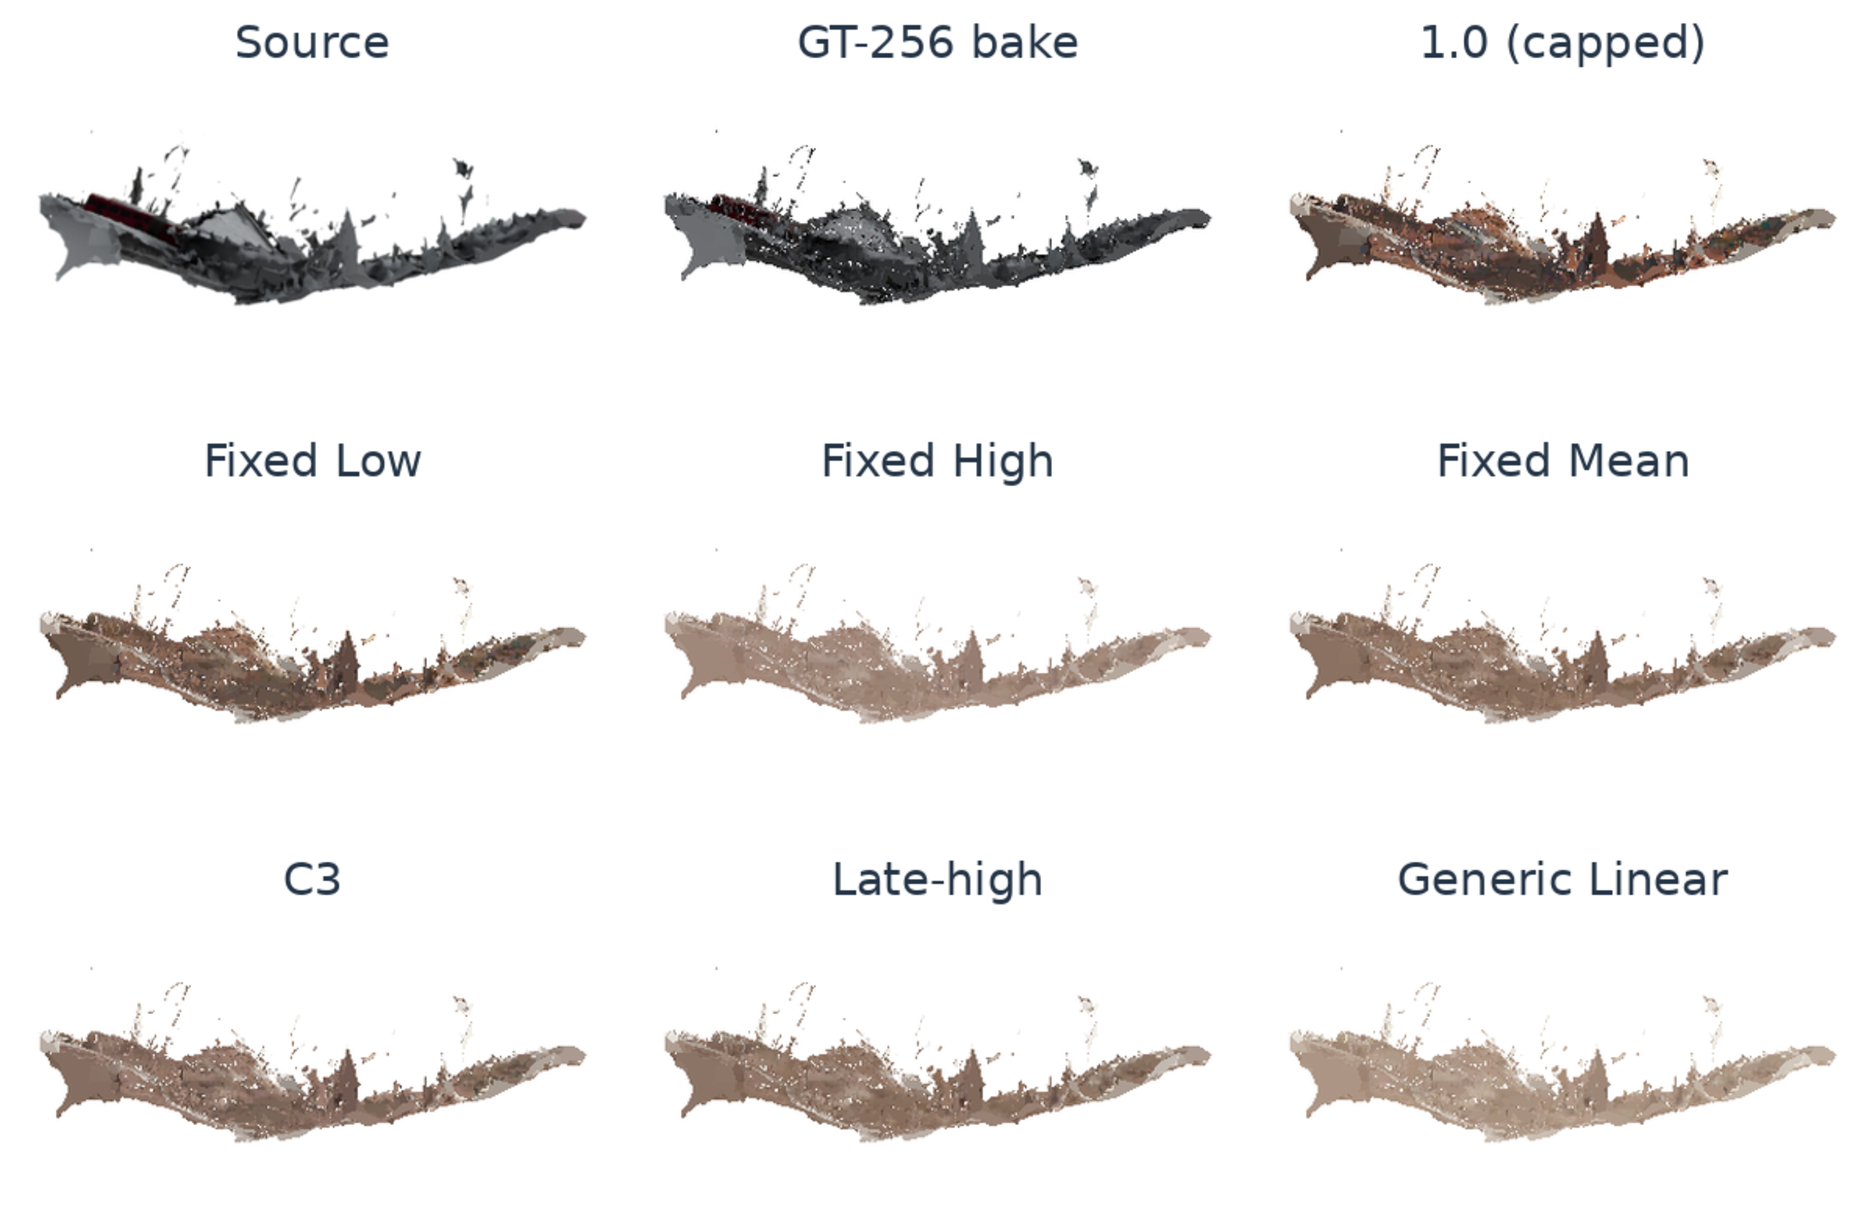
\includegraphics[width=\textwidth,height=0.72\textheight,keepaspectratio]{figures/figS_bake014_05.pdf}
\caption{Rights-cleared GeoTex bake display 5 of seven at unseen camera 004. Source, matched GT-256 reference bake and all seven generated conditions share one whole-object frame.}
\end{figure}

\begin{figure}[p]\centering
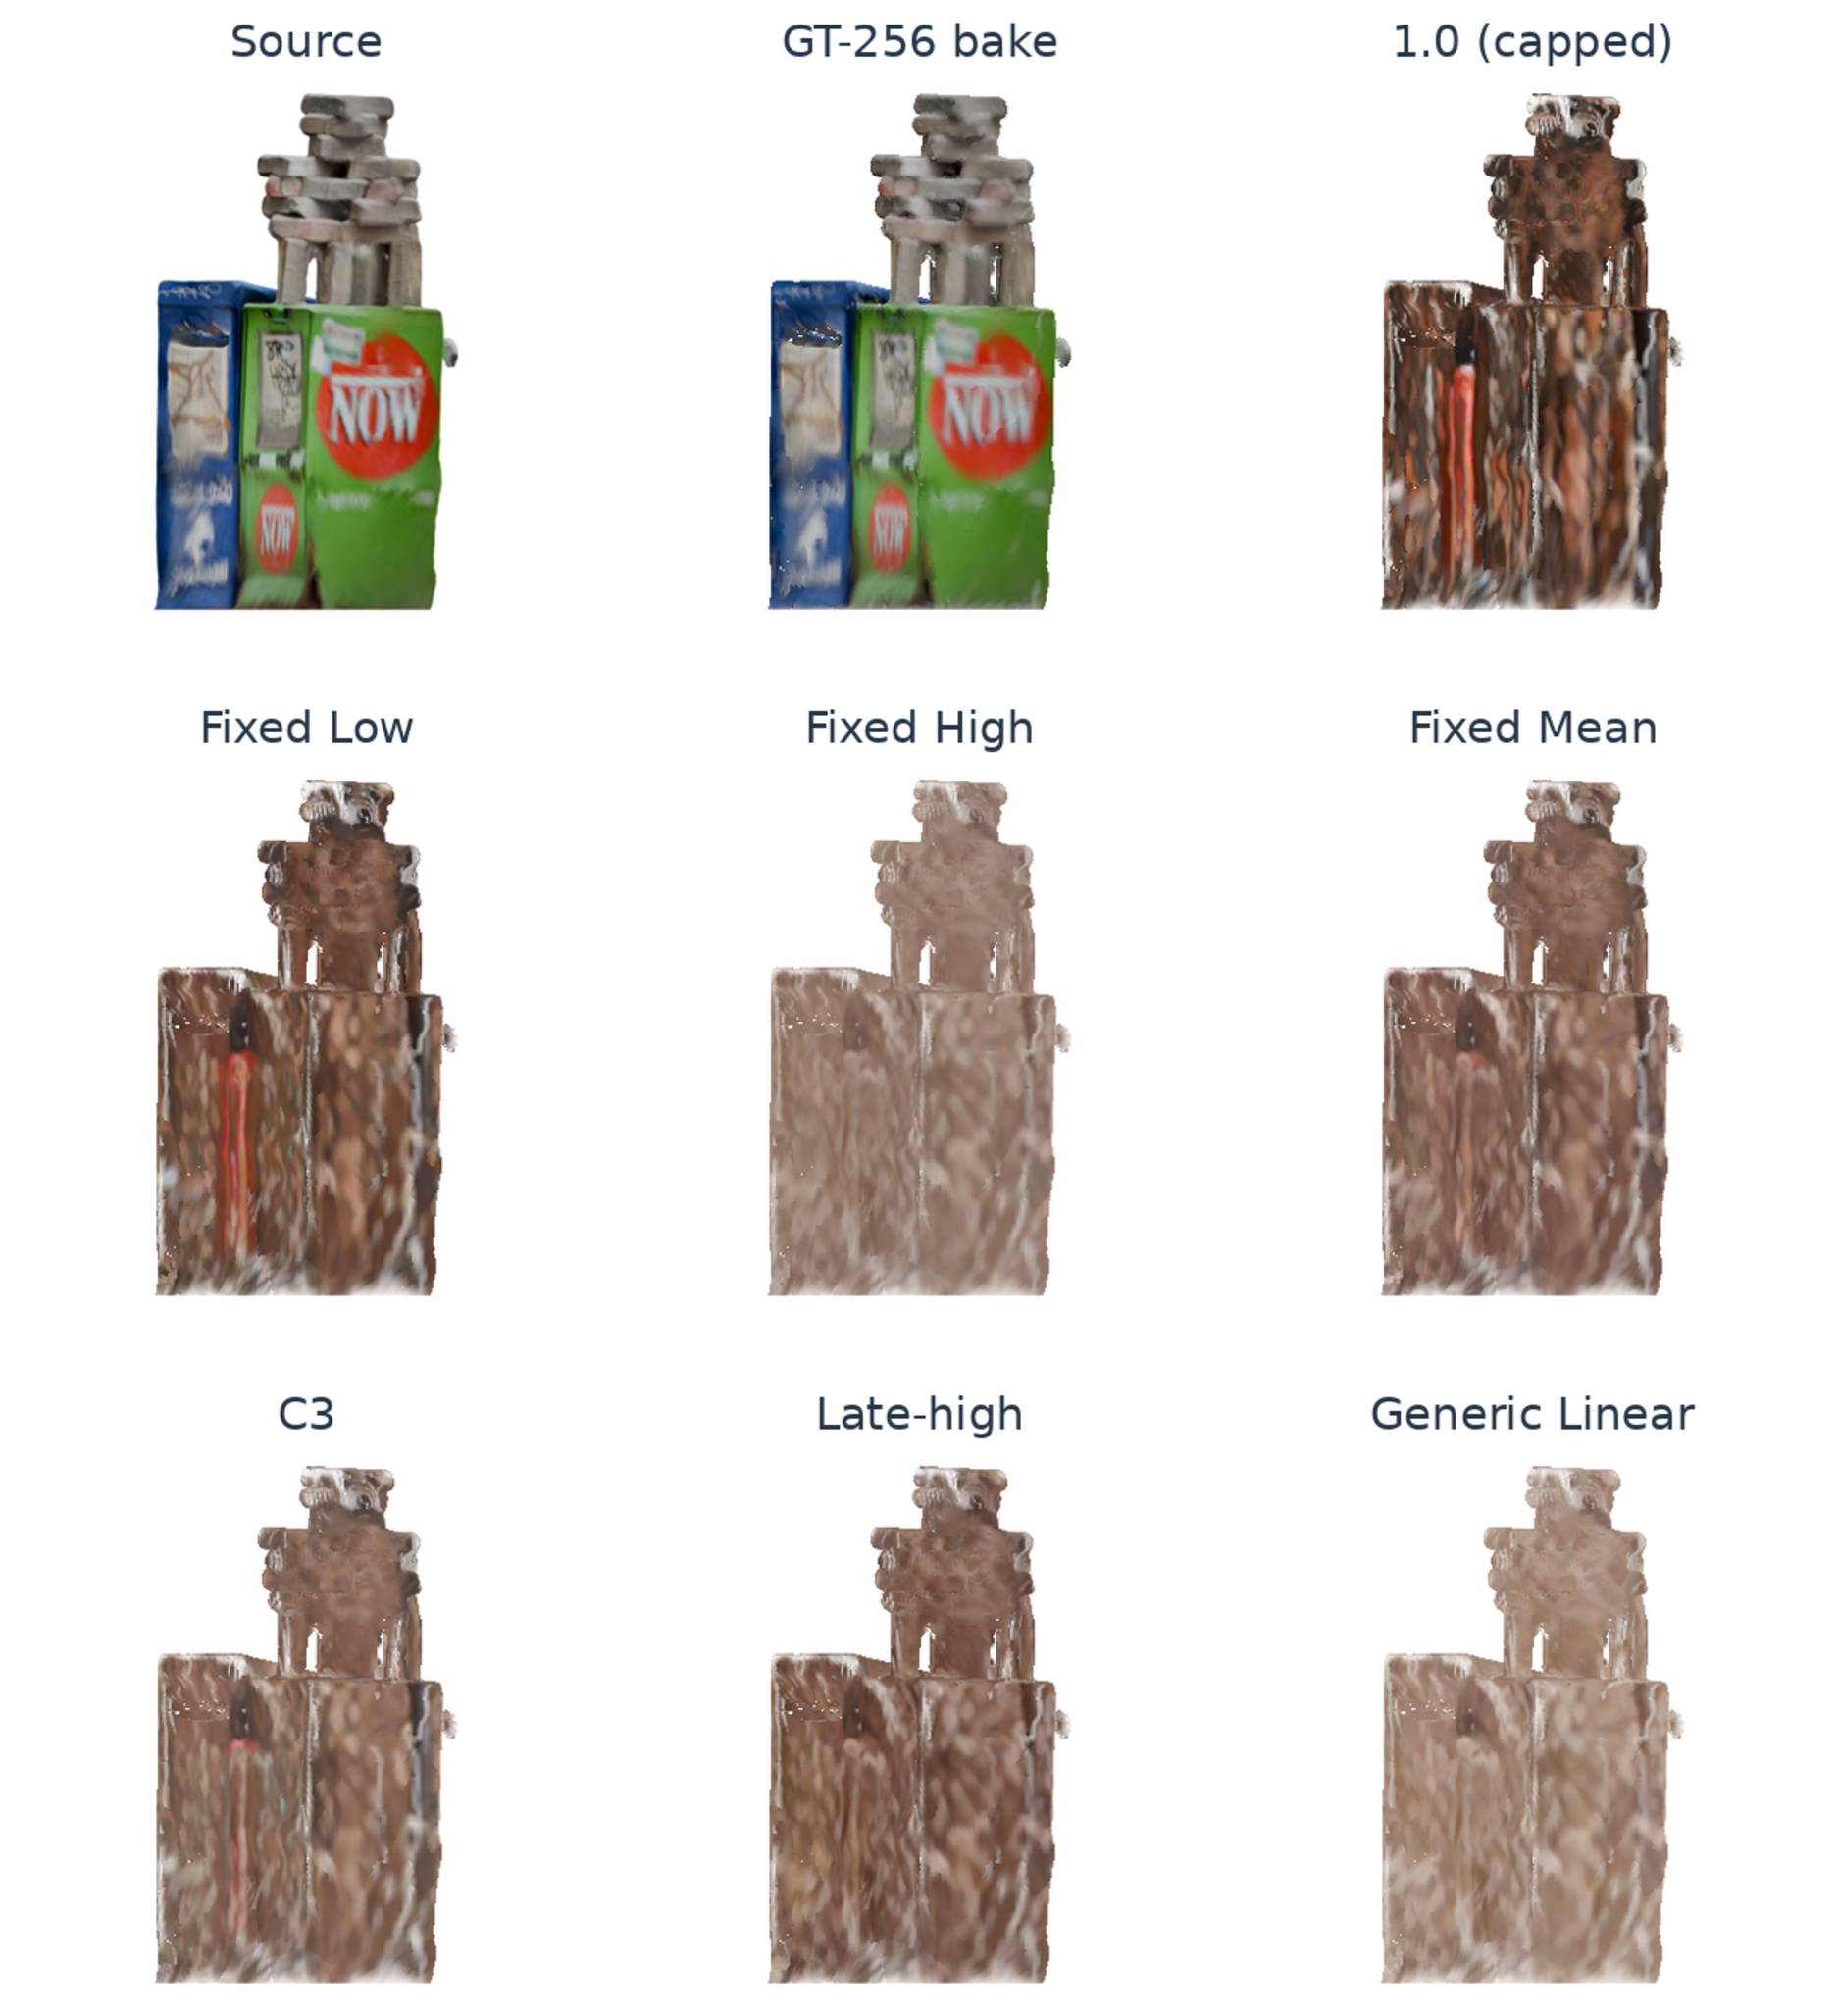
\includegraphics[width=\textwidth,height=0.72\textheight,keepaspectratio]{figures/figS_bake014_06.pdf}
\caption{Rights-cleared GeoTex bake display 6 of seven at unseen camera 004. Source, matched GT-256 reference bake and all seven generated conditions share one whole-object frame.}
\end{figure}

\begin{figure}[p]\centering
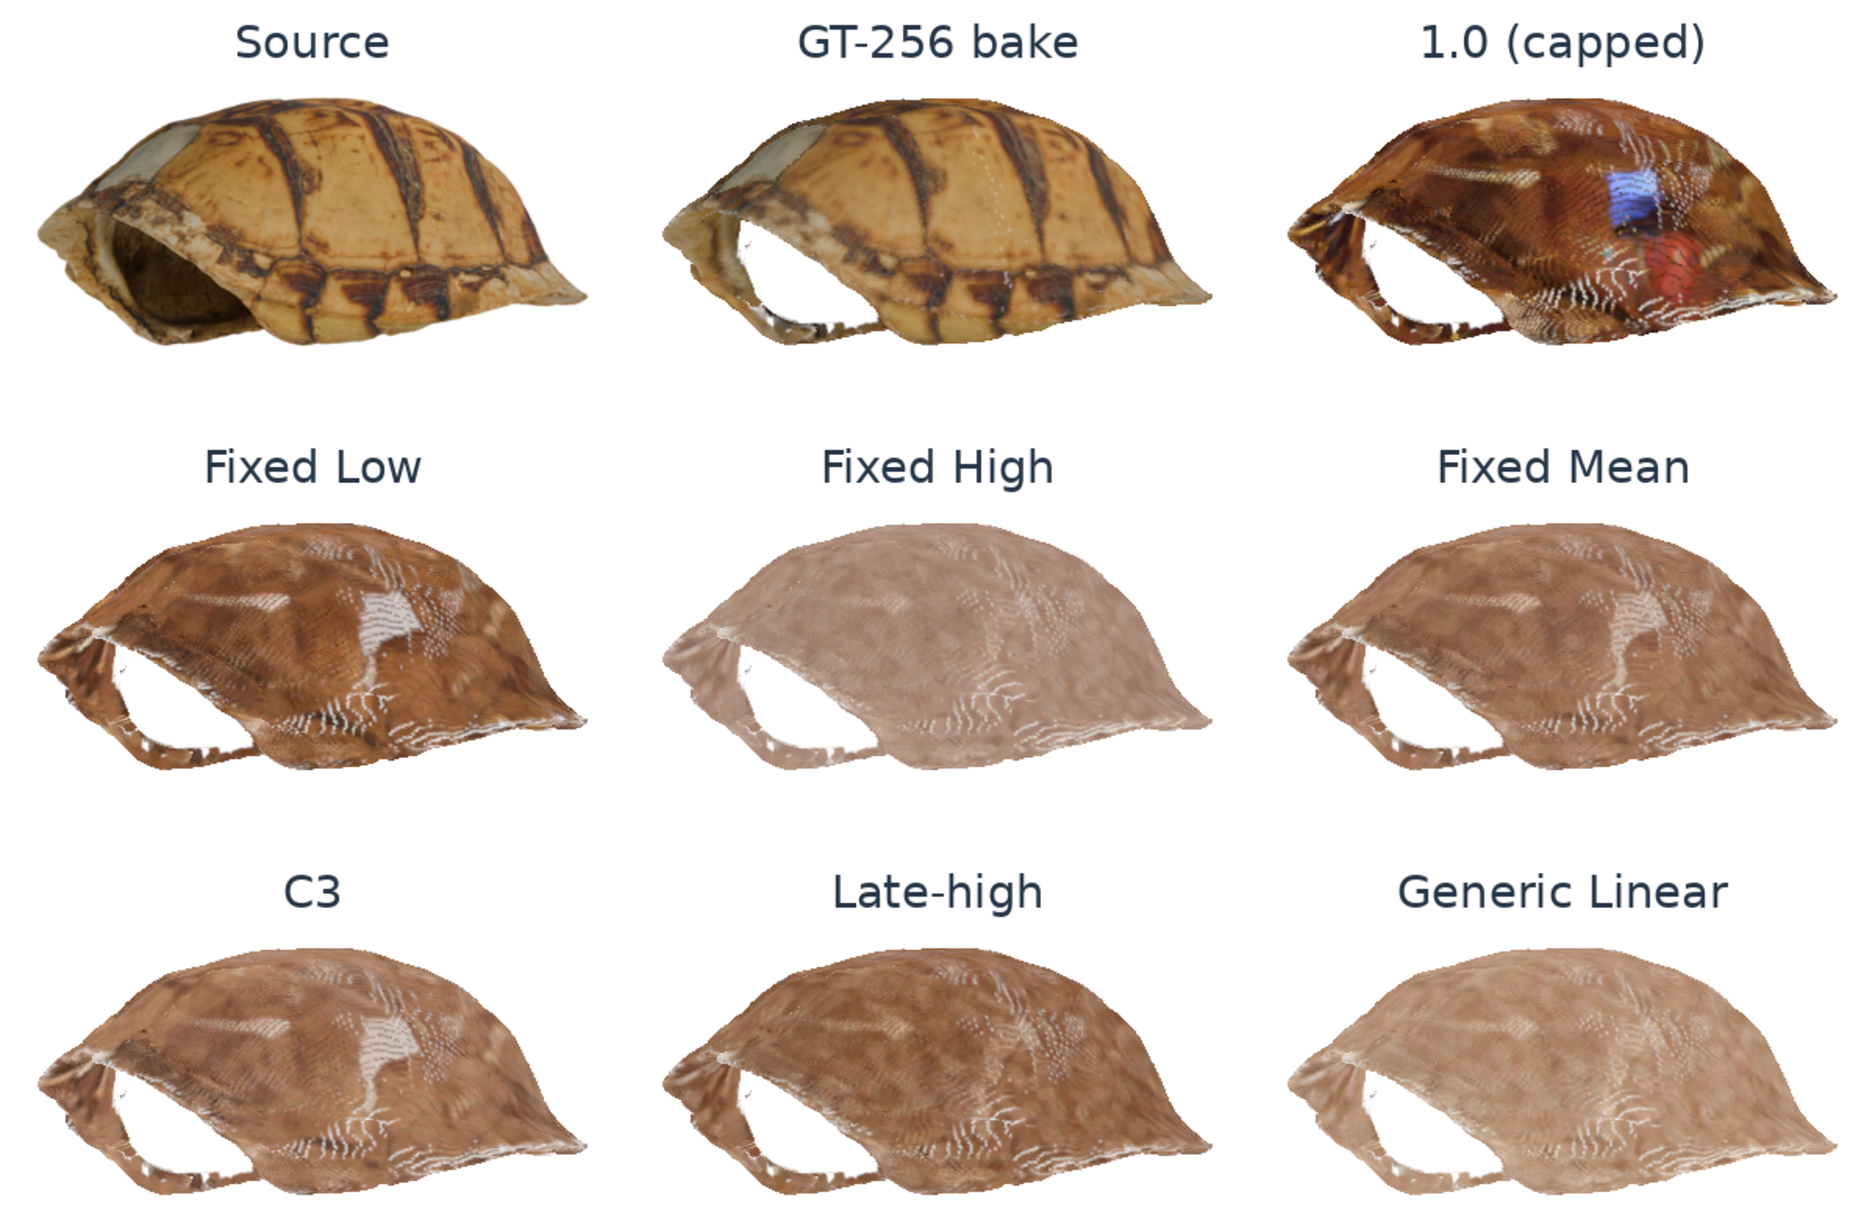
\includegraphics[width=\textwidth,height=0.72\textheight,keepaspectratio]{figures/figS_bake014_07.pdf}
\caption{Rights-cleared GeoTex bake display 7 of seven at unseen camera 004. Source, matched GT-256 reference bake and all seven generated conditions share one whole-object frame.}
\end{figure}


The separately supplied \texttt{Supplementary\_GeoTex\_Baked\_Comparison.mp4} presents two input-order, rights-cleared GeoTex objects at all eleven discrete unseen cameras. Each actual rendered view is held for one second; no interpolated camera image is synthesized. It is an unlit comparison, not a claim of continuous-view or PBR quality.

LG Remote by mohd.akmal.mahyudin; CC Attribution. Source: \url{https://sketchfab.com/3d-models/1dc2c857f7614caeb6c2aa0559ccf973}.

Tire by Koto3D Stephane Vogley; CC Attribution. Source: \url{https://sketchfab.com/3d-models/21678bd623654182b52c11d013de4e71}.

Asset 238ff3e41c964655b83aa9c8770cc766 by suntaree; CC Attribution. Source: \url{https://sketchfab.com/3d-models/238ff3e41c964655b83aa9c8770cc766}.

Baptisimal Font - Aughrim by Galway3D\_DH\_AGe; CC0 Public Domain. Source: \url{https://sketchfab.com/3d-models/2dd9bc8172c6461797947cc7214db399}.

Pittsburgh Bridge Collapse in Frick Park by C8X; CC Attribution. Source: \url{https://sketchfab.com/3d-models/2f6c94487ee54cb88021f4643409d849}.

bricks on news boxes by bunnyhero; CC Attribution. Source: \url{https://sketchfab.com/3d-models/3c83796ca5f043f1beb8044dd2e51a0d}.

Eastern Box Turtle Shell by Frank McMains; CC Attribution. Source: \url{https://sketchfab.com/3d-models/85a7df80b79a4ba9b8c3a175de0dbce6}.


\clearpage

\subsection*{Post hoc GT reference context and object influence}
\addcontentsline{toc}{subsection}{Post hoc GT reference context and object influence}
This reanalysis uses the same valid ten-object source records and the same frozen endpoints; it is not a new holdout or a new confirmatory family. GT-256 is a matched empirical projection reference, not a theoretical upper bound on an image endpoint. Its mean PSNR/LPIPS/SSIM/Edge-SSIM/CIEDE2000 are 22.38/0.0590/0.7683/0.7533/4.44. Late-high's LPIPS gain relative to Fixed Mean is unchanged at 0.00265.

For descriptive magnitude context, the ratio of means is
\[
 r=\frac{\mathrm{mean}(\mathrm{LPIPS}_{Mean}-\mathrm{LPIPS}_{Late})}{\mathrm{mean}(\mathrm{LPIPS}_{Mean}-\mathrm{LPIPS}_{GT256})}=0.03720.
\]
The numerator and denominator are recomputed jointly in each of 50,000 object-bootstrap samples (seed 20261010). All bootstrap denominators are positive; the pointwise interval is [0.02275,0.05323]. This is a roughly 3.7\% reduction of the mean empirical reference gap, not evidence that the remaining appearance mismatch is small. It must not be interpreted as a practical acceptability threshold or a new primary discovery. Removing each object in turn yields Late--Mean mean differences between $-0.00294$ and $-0.00208$; this descriptive influence check does not create additional independent samples.

\begin{longtable}{lrrrr}
\caption{Same ten objects: matched reference and generated unseen-view FG-LPIPS. All eleven unseen views are averaged first. Full UIDs and exact values accompany the reanalysis script.}\\
\toprule UID prefix & GT-256 & Fixed Mean & Late-high & Late--Mean \\
\midrule\endfirsthead
\toprule UID prefix & GT-256 & Fixed Mean & Late-high & Late--Mean \\
\midrule\endhead
1dc2c857f761 & 0.07674 & 0.15307 & 0.14898 & -0.00408 \\
21678bd62365 & 0.07367 & 0.17198 & 0.16919 & -0.00279 \\
238ff3e41c96 & 0.02328 & 0.05895 & 0.05849 & -0.00046 \\
2dd9bc8172c6 & 0.14110 & 0.23763 & 0.22982 & -0.00781 \\
2f6c94487ee5 & 0.06525 & 0.09319 & 0.09317 & -0.00003 \\
3c83796ca5f0 & 0.05597 & 0.17757 & 0.17439 & -0.00318 \\
85a7df80b79a & 0.04051 & 0.10964 & 0.10519 & -0.00445 \\
e261c0fe85af & 0.04032 & 0.13280 & 0.13112 & -0.00168 \\
f1ccc55a65c7 & 0.06034 & 0.11759 & 0.11622 & -0.00137 \\
fa5c4b02c5b2 & 0.01312 & 0.05075 & 0.05010 & -0.00065 \\
\bottomrule\end{longtable}
The script \texttt{scripts/analyze\_gt\_context.py}, copied source CSV and \texttt{GT\_REFERENCE\_CONTEXT.json} permit standalone reproduction with NumPy. No generated output is added, replaced or retouched. The source hash identifies the previous round's valid metrics; historical five, N=20 and invalid old native-seven records remain separate.

\subsection*{Native-wrapper controls and sampling-protocol scope}
\addcontentsline{toc}{subsection}{Native-wrapper controls and sampling-protocol scope}
The exploratory wrapper-control addendum adds native-unset residual and No Adapter controls on the same ten objects, with no change to the earlier seven-condition matrix or its primary comparison. These objects and their earlier outcomes have been inspected, so all added contrasts are exploratory. The native control removes the scale attribute immediately before every actual wrapper invocation, leaving the original forward function, geometry features and reference-write skipping logic intact. A regenerated Constant 1.0 (capped) control matches the earlier RGB outputs bitwise on all ten objects; inputs and seeds also match. This identifies the default residual branch within the frozen protocol, not an unmodified complete pipeline.

A read-only source audit identifies additional differences. The frozen generator makes one conditional score prediction per denoising step, uses cached global image embeddings, and generates 256-pixel views. The full base-pipeline call defaults to 512-pixel views, online global embeddings, and classifier-free guidance of 2.0; its denoising loop combines conditional and unconditional predictions. The GeoTex model's validation call uses 75 steps and does not explicitly bind geometry features. Source differences alone cannot identify the cause of the appearance failures or validate a repair. The corresponding source hashes and audit assertions are delivered in \texttt{ITERATION002\_SAMPLING\_PROTOCOL\_AUDIT.json}.

\begin{figure}[htbp]
\centering
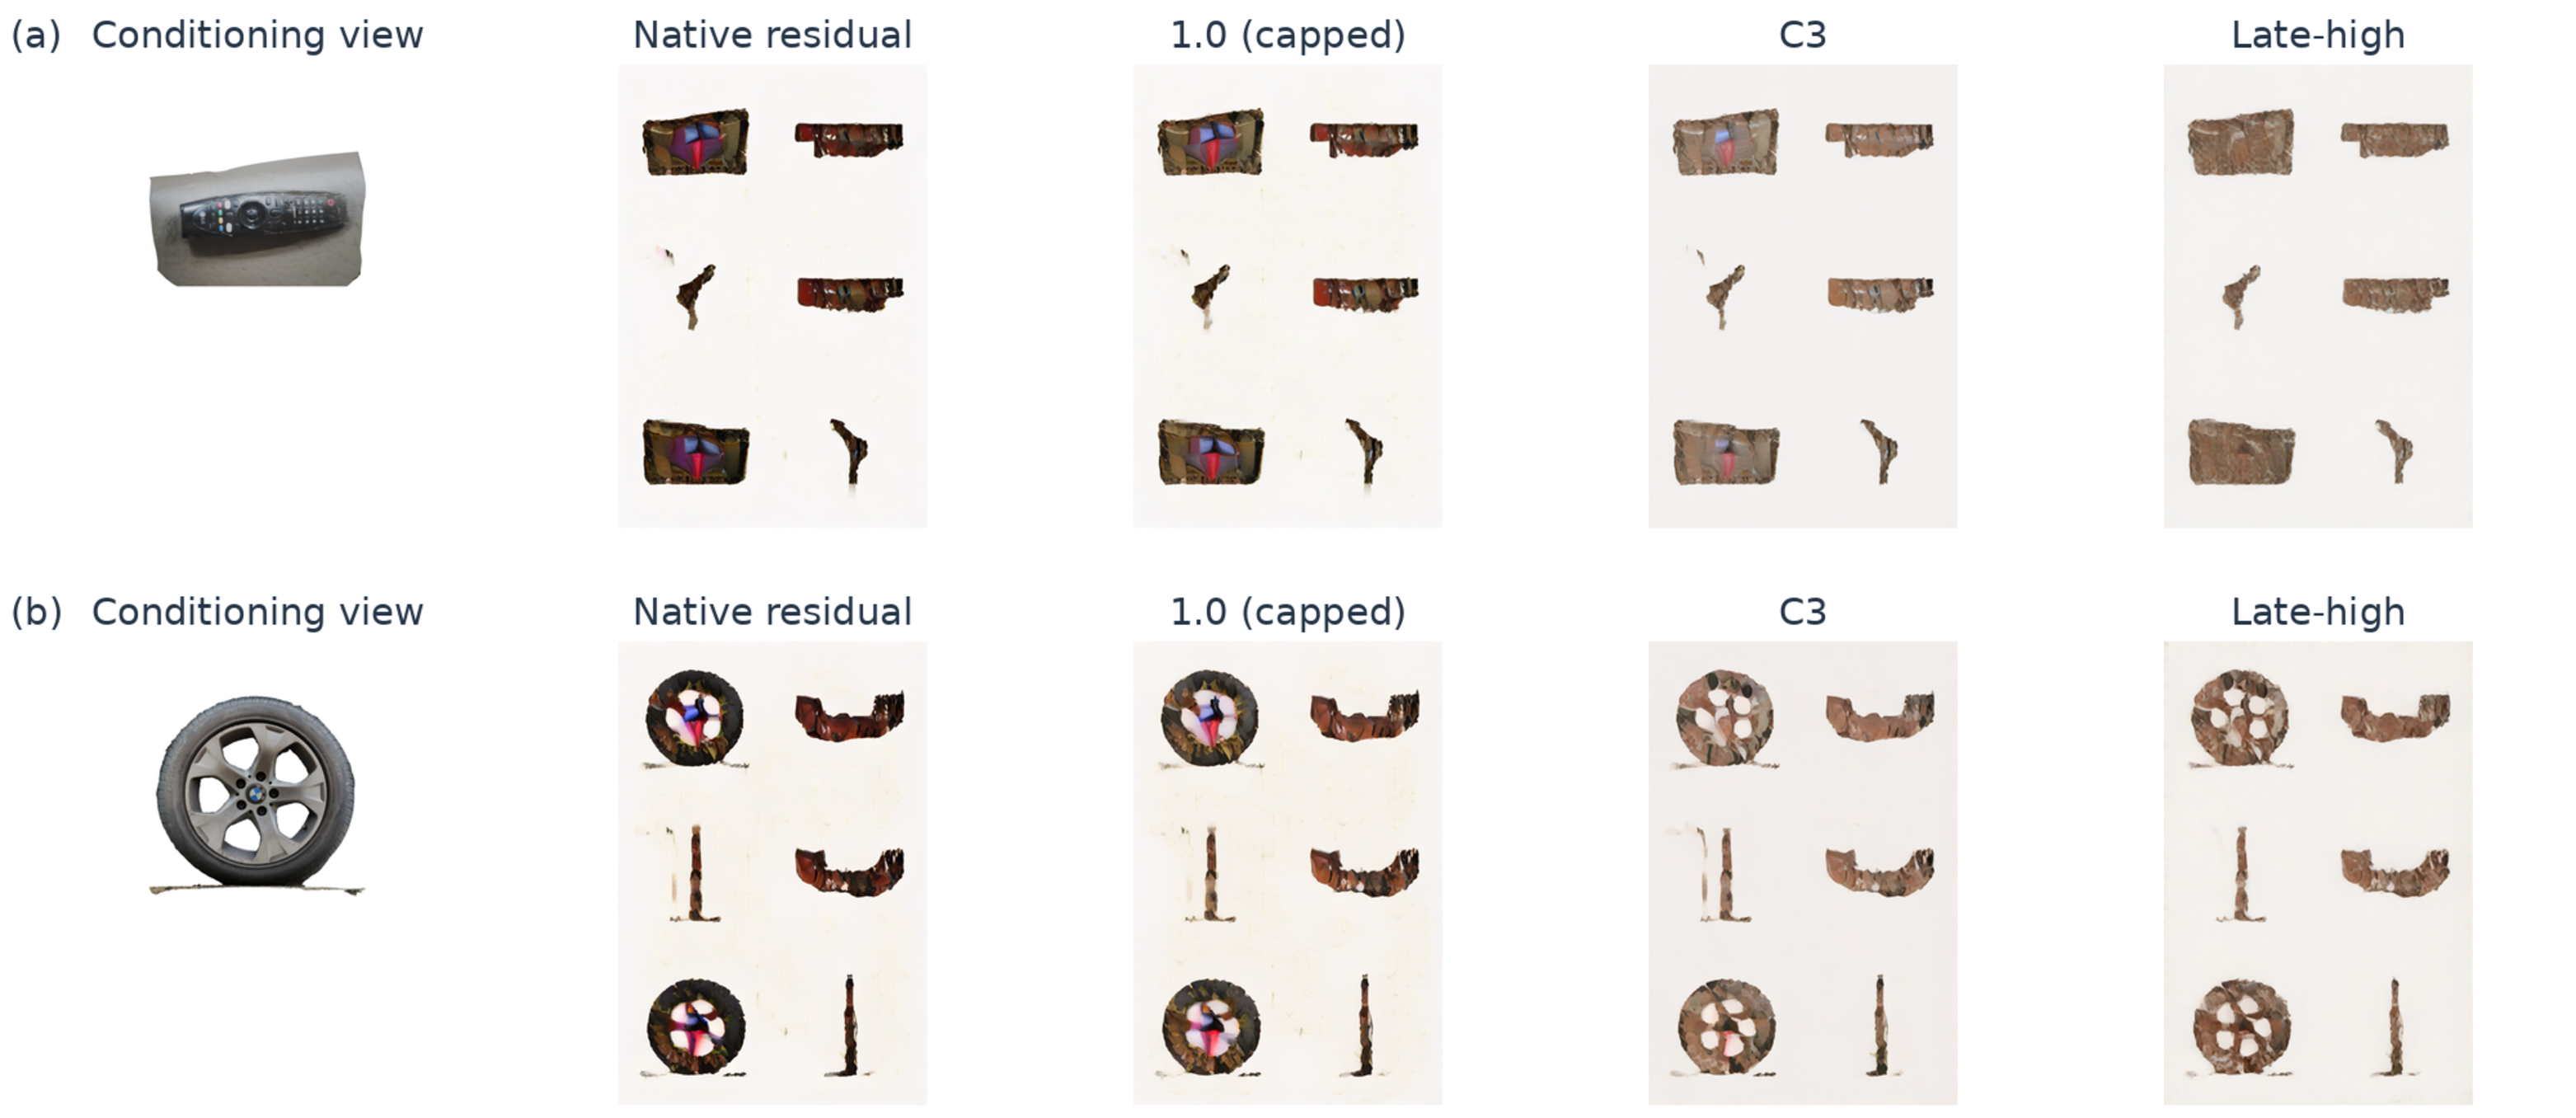
\includegraphics[width=\linewidth,height=0.74\textheight,keepaspectratio]{figures/figS_native_controls014.pdf}
\caption{Generated six-view grids for the same first two input-ordered, rights-cleared objects used in the earlier bake display. The malformed No Adapter visual column is omitted; all its numerical contrasts remain reported. The conditioning image is shown separately. Native residual means the unset-scale wrapper branch in the frozen sampling protocol; it does not mean the complete default pipeline. All grids retain their original contents, with only whole-grid resizing; visible color and detail failures are not retouched. LG Remote: mohd.akmal.mahyudin; Tire: Koto3D Stephane Vogley; both CC Attribution. Full source links are given in S5; new output hashes and credits accompany this figure.}
\end{figure}


\subsection*{Complete exploratory contrast family}\label{supp:bake-native-exploratory}
\addcontentsline{toc}{subsection}{Complete exploratory contrast family}
Each row is A minus Native residual. Higher PSNR/SSIM/Edge-SSIM and lower LPIPS/CIEDE2000 are favorable. The 95\% intervals are pointwise object-bootstrap intervals; adjusted $p$ values belong to one 15-test Holm family. All ten objects are retained, and eleven unseen views are averaged per object. The prior Late-high--Fixed Mean primary remains unchanged. Repeated GT metrics match the earlier evaluation exactly (maximum absolute difference 0).

\begin{table}[htbp]\centering\scriptsize
\begin{tabular}{llrrr}\toprule A & Endpoint & Mean difference & Pointwise 95\% CI & Holm $p$\\\midrule
Late-high & FG-PSNR & $+1.78764$ & $[+0.46170,+3.05975]$ & 0.29688 \\
Late-high & FG-LPIPS & $-0.00951$ & $[-0.01772,-0.00263]$ & 0.29688 \\
Late-high & FG-SSIM & $+0.08825$ & $[+0.05443,+0.12228]$ & 0.05469 \\
Late-high & Edge-SSIM & $+0.04958$ & $[+0.02256,+0.07663]$ & 0.12305 \\
Late-high & CIEDE2000 & $-4.82018$ & $[-8.66554,-0.65098]$ & 0.29688 \\
C3 & FG-PSNR & $+1.34525$ & $[+0.13241,+2.56138]$ & 0.29688 \\
C3 & FG-LPIPS & $-0.00699$ & $[-0.01326,-0.00159]$ & 0.29688 \\
C3 & FG-SSIM & $+0.06827$ & $[+0.04193,+0.09422]$ & 0.05469 \\
C3 & Edge-SSIM & $+0.03526$ & $[+0.01168,+0.05974]$ & 0.29688 \\
C3 & CIEDE2000 & $-4.30778$ & $[-7.73875,-0.53688]$ & 0.29688 \\
No Adapter & FG-PSNR & $-5.21580$ & $[-6.60353,-3.61839]$ & 0.05469 \\
No Adapter & FG-LPIPS & $+0.02281$ & $[+0.01287,+0.03317]$ & 0.05469 \\
No Adapter & FG-SSIM & $+0.04520$ & $[-0.02288,+0.11851]$ & 0.29688 \\
No Adapter & Edge-SSIM & $-0.21789$ & $[-0.26399,-0.16852]$ & 0.02930 \\
No Adapter & CIEDE2000 & $+14.44690$ & $[+6.37338,+22.12900]$ & 0.07812 \\
\bottomrule\end{tabular}
\caption{All added object-paired exploratory contrasts. These are previously inspected objects, not a new independent confirmation sample.}\end{table}
No Adapter versus Native residual Edge-SSIM is the sole adjusted rejection in this family. The favorable schedule means and pointwise intervals do not establish family-corrected schedule advantages or acceptable appearance fidelity. The generated-view controls also retain conspicuous color/detail failures in the displayed examples.

\subsection*{Historical N=20 unseen-view results}
\addcontentsline{toc}{subsection}{Historical N=20 unseen-view results}
Table~\ref{tab:supp-n20} reports the bounded historical N=20 GLB results. The subset comprises 20 UV-compatible objects from the original 24-object pool; four inputs were excluded for lack of UVs. Each object is the paired unit after averaging 11 frozen unseen views. Rendering uses unlit base color with native sampler interpretation. Endpoint directions are mixed; these statistics do not establish population-level 3D superiority, PBR/material fidelity, seam quality, or human preference. The source GLB assets and internal montage are not included in this supplement.
\begin{table}[ht]
\centering\small
\caption{Historical N=20 unlit base-color paired unseen-view summaries (C3 minus comparator). The 20-object UV-compatible subset comes from the historical 24-object pool; four objects were excluded for missing UVs. Each object is averaged over 11 frozen unseen views. Intervals are 10,000-object-bootstrap percentile CIs (seed 20261005), descriptive and unadjusted.}\label{tab:supp-n20}
\begin{tabular}{llcc}\toprule Comparator & Endpoint & Mean difference [95\% CI] & Objects favoring C3 \\\midrule
GFL & FG-PSNR (dB) & -0.066 [-0.413, +0.290] & 5/20 (25\%) \\
GFL & FG-LPIPS & -0.004719 [-0.007504, -0.002544] & 17/20 (85\%) \\
GFL & CIEDE2000 & +0.133 [-1.161, +1.319] & 6/20 (30\%) \\
GFH & FG-PSNR (dB) & +0.084 [-0.290, +0.426] & 14/20 (70\%) \\
GFH & FG-LPIPS & +0.007709 [+0.004230, +0.012101] & 4/20 (20\%) \\
GFH & CIEDE2000 & -1.027 [-2.224, +0.229] & 14/20 (70\%) \\
No Adapter & FG-PSNR (dB) & +3.135 [+1.721, +4.493] & 18/20 (90\%) \\
No Adapter & FG-LPIPS & -0.014519 [-0.029860, -0.001326] & 16/20 (80\%) \\
No Adapter & CIEDE2000 & -12.508 [-18.556, -6.529] & 18/20 (90\%) \\
\bottomrule\end{tabular}
\end{table}

\subsection*{Unresolved 3D checks}
\addcontentsline{toc}{subsection}{Unresolved 3D checks}



The attempted Fresh C 24-object GLB bake did not pass its input/output gate: 9/24 sources had out-of-range native UVs, and 5 assets / 27 primitives used unsupported BLEND. No valid Fresh C 24-object bake results were generated. The seam endpoint is retired because the required seam truth set and native full-panel validation did not pass. No full PBR comparison is available. These checks are limitations, not evidence of method failure or success.

\FloatBarrier
\subsection*{Incoming-camera disagreement on shared UV texels}
\addcontentsline{toc}{subsection}{Incoming-camera disagreement on shared UV texels}
This additional diagnostic uses the already recorded source-view projection, before filling holes or rendering the exported atlas. For camera $v$ and texel $t$, let $c_{vt}$ be its linear-RGB average after visible-pixel bilinear UV splatting. Let $V_t$ be the cameras with accumulated weight exceeding $10^{-8}$. We retain only texels with $|V_t|\geq2$, average cameras equally within each texel and then average population channel variance equally across the retained texels:
\[
D=\frac{1}{3|T|}\sum_{t\in T}\sum_{k=1}^3\left[\frac{1}{|V_t|}\sum_{v\in V_t}c_{vtk}^{2}-\left(\frac{1}{|V_t|}\sum_{v\in V_t}c_{vtk}\right)^2\right]_+ .
\]
The nonnegative clamp handles rounding. One-camera texels do not contribute. Six original cameras, GT-256 resolution/masks, 1024 atlas, original material and sampler, and the repaired REPEAT interpolation are shared with the bake. We copied the actual archived baker with SHA256 \texttt{f7eeb7cc4efb166cd4138b832e91356f36f775ac18badedefde5610aafdb8db4}, rather than silently substituting a later implementation. All 80 previously recorded values reproduce exactly.

On the first two input-order objects, known camera-constant gray inputs ($c_v=v/5$, $v=0,\ldots,5$) yield 0.12721819 and 0.12461645; independent camera-incidence calculations agree to at most $1.1\times10^{-8}$. A shared constant-black input gives exactly zero in both cases. The diagnostic can therefore return perfect agreement for an incorrect, flat appearance. These controlled input substitutions are formula/path checks, not newly generated model outputs or quality evidence. Inputs and original method images are unaltered.

\begin{table}[ht]\centering\small
\caption{Ten-object recorded incoming-camera variance and actual baked LPIPS means. GT-256 is a path reference, not a perfect oracle. Lower disagreement does not imply better reference agreement.}\label{tab:cross-view015}
\begin{tabular}{lrr}\toprule Condition & Shared-UV variance & Unseen FG-LPIPS \\
\midruleConstant 1.0 (capped) & 0.028847 & 0.13537 \\
Fixed Low & 0.025736 & 0.13168 \\
Fixed High & 0.010888 & 0.13055 \\
Fixed Mean & 0.019640 & 0.13032 \\
C3 / Middle-high & 0.022242 & 0.13018 \\
Late-high & 0.017192 & 0.12767 \\
Generic Linear & 0.012625 & 0.12763 \\
GT-256 & 0.001787 & 0.05903 \\
\bottomrule\end{tabular}
\end{table}
Late--Mean variance is $-0.002448$ (pointwise descriptive interval $[-0.003473,-0.001604]$; all ten negative). Its exact sign-flip $p=0.001953$ becomes 0.041016 in the additional 21-pair Holm family. This family was specified after seeing the original bake endpoints and is exploratory. The two tested color controls do not certify arbitrary assets: UV overlap/repetition, natural texture, source-view dependence and sampling can produce disagreement. No quantitative seam or PBR endpoint is validated.

\begin{longtable}{p{.43\textwidth}rrr}
\caption{All generated-condition pairs for the additional shared-UV diagnostic. A minus B; pointwise descriptive object intervals, 20,000 draws with seed 20261012; exact $2^{10}$ paired sign flips and one Holm21 family.}\label{tab:cross-view-all015}\\
\toprule Contrast & Mean & 95\% interval & Holm $p$ \\
\midrule\endfirsthead\toprule Contrast & Mean & 95\% interval & Holm $p$ \\
\midrule\endhead
Constant 1.0 (capped) -- Fixed Low & $+0.003111$ & $[+0.001548,+0.004773]$ & 0.04102 \\
Constant 1.0 (capped) -- Fixed High & $+0.017959$ & $[+0.011968,+0.024607]$ & 0.04102 \\
Constant 1.0 (capped) -- Fixed Mean & $+0.009208$ & $[+0.005554,+0.012970]$ & 0.04102 \\
Constant 1.0 (capped) -- C3 / Middle-high & $+0.006606$ & $[+0.003810,+0.009709]$ & 0.04102 \\
Constant 1.0 (capped) -- Late-high & $+0.011656$ & $[+0.007678,+0.015919]$ & 0.04102 \\
Constant 1.0 (capped) -- Generic Linear & $+0.016222$ & $[+0.010458,+0.022681]$ & 0.04102 \\
Fixed Low -- Fixed High & $+0.014848$ & $[+0.009782,+0.020292]$ & 0.04102 \\
Fixed Low -- Fixed Mean & $+0.006097$ & $[+0.003672,+0.008454]$ & 0.04102 \\
Fixed Low -- C3 / Middle-high & $+0.003495$ & $[+0.001986,+0.005090]$ & 0.04102 \\
Fixed Low -- Late-high & $+0.008545$ & $[+0.005577,+0.011622]$ & 0.04102 \\
Fixed Low -- Generic Linear & $+0.013111$ & $[+0.008330,+0.018323]$ & 0.04102 \\
Fixed High -- Fixed Mean & $-0.008752$ & $[-0.012033,-0.005831]$ & 0.04102 \\
Fixed High -- C3 / Middle-high & $-0.011354$ & $[-0.015333,-0.007696]$ & 0.04102 \\
Fixed High -- Late-high & $-0.006304$ & $[-0.008839,-0.004094]$ & 0.04102 \\
Fixed High -- Generic Linear & $-0.001737$ & $[-0.002234,-0.001269]$ & 0.04102 \\
Fixed Mean -- C3 / Middle-high & $-0.002602$ & $[-0.003464,-0.001571]$ & 0.04102 \\
Fixed Mean -- Late-high & $+0.002448$ & $[+0.001604,+0.003473]$ & 0.04102 \\
Fixed Mean -- Generic Linear & $+0.007015$ & $[+0.004426,+0.010028]$ & 0.04102 \\
C3 / Middle-high -- Late-high & $+0.005050$ & $[+0.003460,+0.006721]$ & 0.04102 \\
C3 / Middle-high -- Generic Linear & $+0.009617$ & $[+0.006251,+0.013327]$ & 0.04102 \\
Late-high -- Generic Linear & $+0.004567$ & $[+0.002643,+0.006902]$ & 0.04102 \\

\bottomrule\end{longtable}

\FloatBarrier
\section*{S6. Appearance failures and executed-protocol diagnostics}
\label{supp:group6}
\addcontentsline{toc}{section}{S6. Appearance failures and executed-protocol diagnostics}

\subsection*{Paired color-pathway diagnosis and failure boundaries}
\addcontentsline{toc}{subsection}{Paired color-pathway diagnosis and failure boundaries}
The color diagnosis is a selected, failure-enriched set of six earlier cases and 20 Fresh C panels; it is neither random nor a new holdout. No Adapter, GFL, and LLH were compared on the same inputs, checkpoint, and runner across six unique target views (78 object-condition records). CIEDE2000 was recomputed from hash-identified RGB and frozen masks. Intervals are descriptive paired object bootstraps (20,000 resamples, seed 61008); no confirmatory multiplicity family was defined. The main manuscript's Figure 4 shows Cap Test -- PhotoCatch (UID \texttt{66ea60ce156e4815964dde27c196b9e5}) as a separate visual comparison.

\begin{table}[ht]
\centering\scriptsize
\caption{Selected paired endpoints from the failure-enriched 26-object color diagnosis. Each row is condition A minus B with an object-level 95\% paired-bootstrap CI. Lower CIEDE2000 and FG-LPIPS are favorable; higher PSNR and Edge-SSIM are favorable. Local texture statistics describe variation, not fidelity.}
\label{tab:color-diagnostic}
\begin{tabular}{llrr}
\toprule Contrast & Endpoint & Mean difference & 95\% CI \\
\midrule
GFL -- No Adapter & Foreground CIEDE2000 & $-19.654$ & [$-26.370,-13.248$] \\
GFL -- No Adapter & FG-PSNR (dB) & $+6.646$ & [$+5.556,+7.635$] \\
GFL -- No Adapter & FG-LPIPS & $-0.03251$ & [$-0.05363,-0.01072$] \\
GFL -- No Adapter & Edge-SSIM & $+0.06510$ & [$+0.04853,+0.08202$] \\
LLH -- GFL & Foreground CIEDE2000 & $+3.583$ & [$+0.462,+6.712$] \\
LLH -- GFL & FG-PSNR (dB) & $-0.197$ & [$-1.562,+1.297$] \\
LLH -- GFL & FG-LPIPS & $-0.01294$ & [$-0.02742,+0.00066$] \\
LLH -- GFL & Edge-SSIM & $-0.00080$ & [$-0.00776,+0.00659$] \\
LLH -- GFL & Foreground gradient magnitude & $-0.06772$ & [$-0.08132,-0.05494$] \\
LLH -- GFL & Foreground high-frequency energy & $-0.00887$ & [$-0.01091,-0.00672$] \\
LLH -- GFL & Foreground color entropy & $-0.598$ & [$-0.703,-0.502$] \\
\bottomrule
\end{tabular}
\end{table}

GFL lowered reference-relative CIEDE2000 in 24/26 objects, but visible pink or purple remained in two legacy cases under all three conditions. LLH increased mean color error while reducing local variation, not fidelity. The RGB shift was visible before baking and at denoising update 40. For one case, a ground-truth VAE round trip gave CIEDE2000 4.086 and $\Delta a^*\approx-1.35$, versus 22.032 and $+1.977$ for GFL; this weakens a VAE-only explanation but does not identify the cause.

A locked P0 trace of three preselected objects reproduced saved RGB pixels exactly in repeated Python 3.13.5 runs; Python 3.10 reproduced its corresponding archived observer. The first cross-runtime tensor difference followed multiplication of the shared FP16 initial latent by the scheduler noise scale (maximum absolute difference 0.0625; RMSE 0.00966; 32.3\% changed). This resolves output identity only for these three traces; it establishes neither cohort-wide cross-stack equivalence nor the color cause.

The feature-relative residual gate increased mean CIEDE2000 by 1.35 across 26 objects and 3.18 in the six earlier cases, with no clear visual improvement. The complete cause remains unresolved; no repair is validated.

\subsection*{Native base-pipeline protocol and two-object diagnostic}
\addcontentsline{toc}{subsection}{Native base-pipeline protocol and two-object diagnostic}
The complete native base-pipeline diagnostic uses the same two previously inspected, rights-cleared failure objects, not an independent confirmation cohort. We load the identical native base model assets directly, without GeoTex weights or geometry residuals, and call the complete pipeline at 50 and 75 steps. All four calls generate 1024$\times$1536 grids (six 512-pixel views). Observation hooks record exactly 50/75 actual UNet calls, each with the two-member classifier-free batch; the 50/75 starting latents match within each object. The scheduler is the native EulerAncestralDiscreteScheduler with trailing timesteps. The previously supplied batch conditioning hashes match, establishing source correspondence rather than full preprocessing equivalence.

The first RGB API attempt fails before any output because the native recenter helper expects four channels. It is preserved separately. The valid second attempt uses the original single-reference RGBA source. Native preprocessing mutates some white foreground pixels in place; the before/after input images are archived. Source inspection also identifies an incompatible validation entry in the GeoTex model: it wraps the UNet while the full pipeline's preparation entry asserts a bare UNet. This is a source-level finding, not a reported execution of the complete GeoTex validation path. Independent native base loading avoids that incompatibility without changing the pipeline's denoising code.

The frozen generator's image inverse scaling is $1.6x$, followed by $0.5x+0.5$, yielding $0.8x+0.5$. The full pipeline composes the same two factors. The formulas are algebraically equal; naming differences do not demonstrate a decoding error.

\begin{figure}[p]\centering
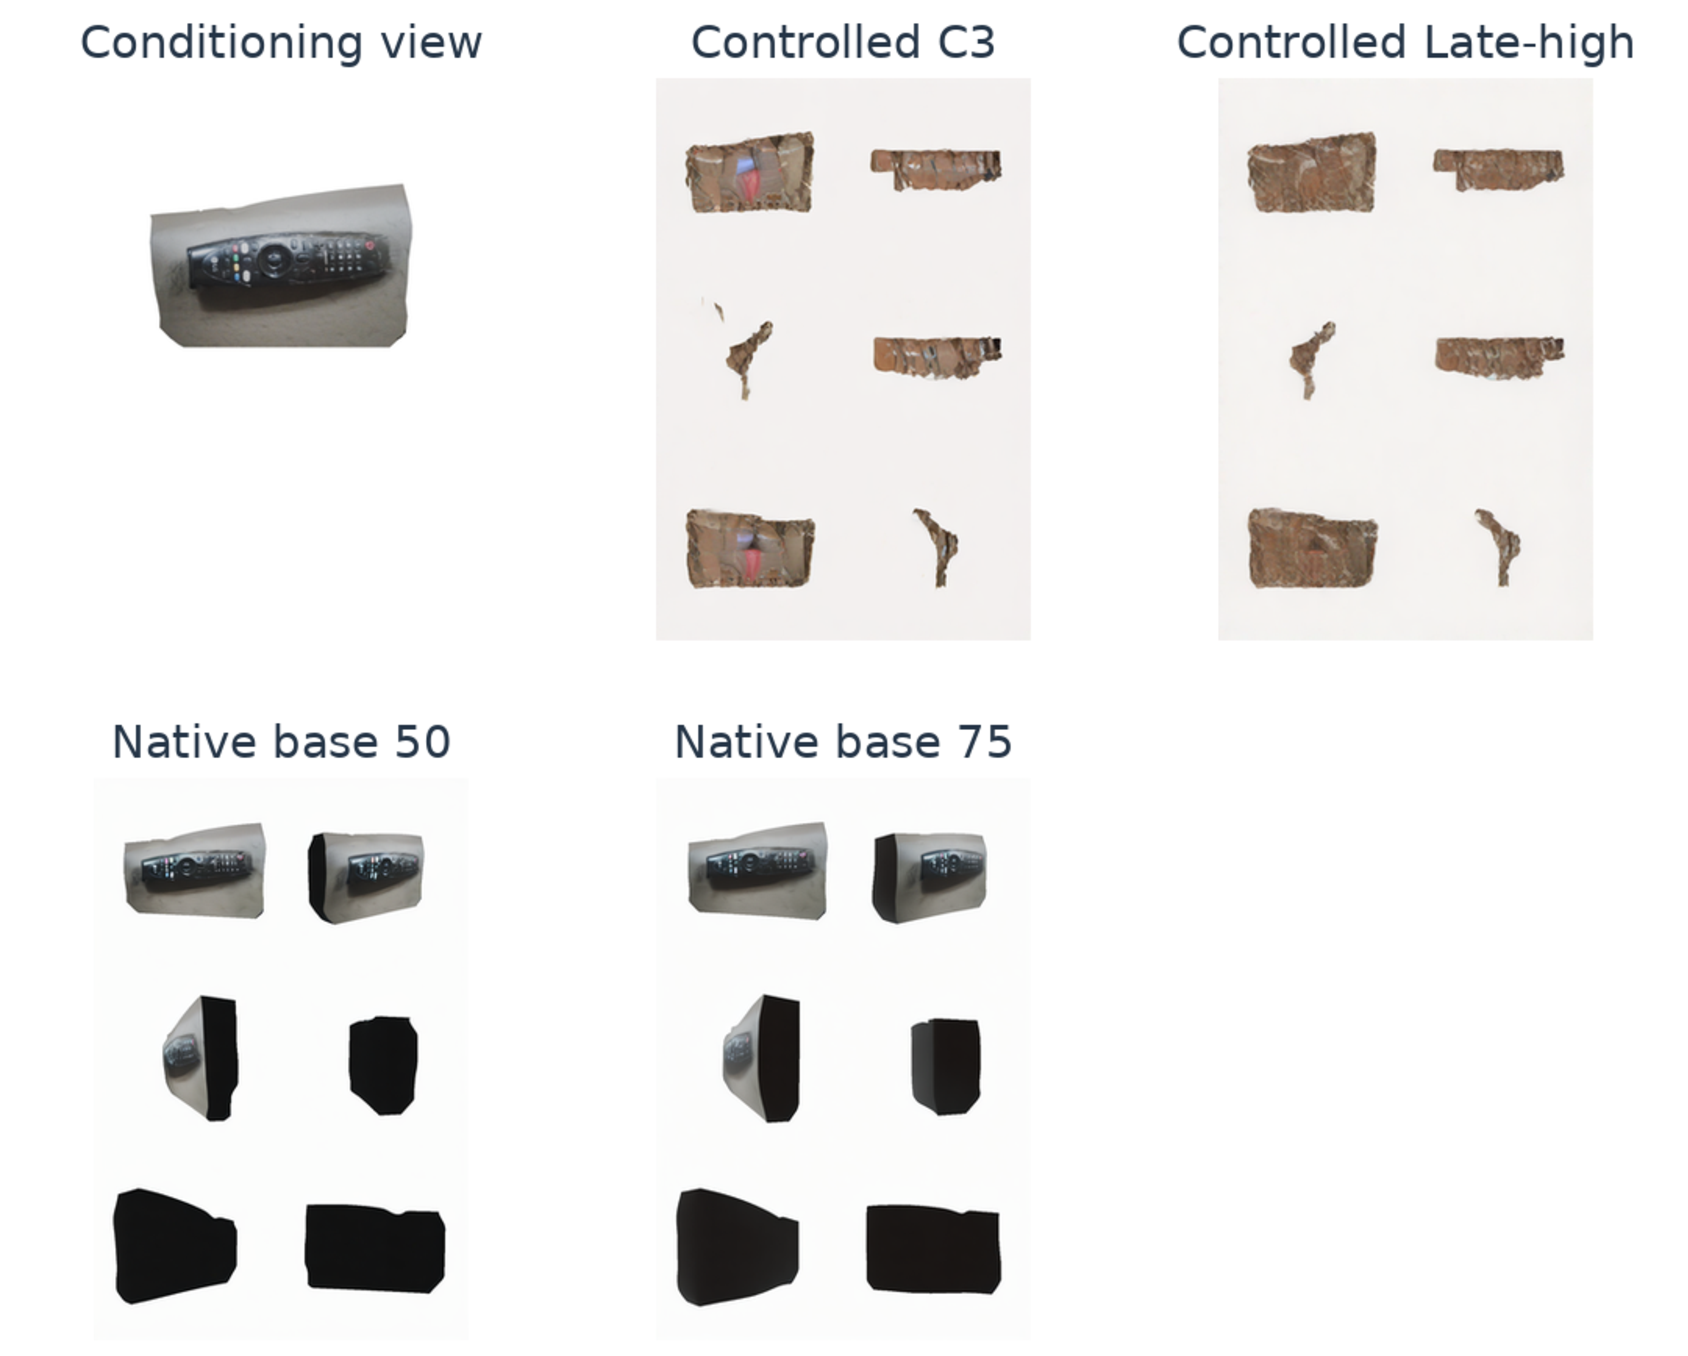
\includegraphics[width=\linewidth,height=0.72\textheight,keepaspectratio]{figures/figS_base_diagnostic014_01.pdf}
\caption{Retained complete grids for a fixed input-order failure object. The disabled-adapter visual column is omitted; its records remain available. Native base outputs use a different sampler and unverified camera conventions, so these are protocol diagnostics rather than aligned GT comparisons or complete default GeoTex results. No reference-fidelity inference follows from the better front-looking native color. Object 1 of two.}
\end{figure}

\begin{figure}[p]\centering
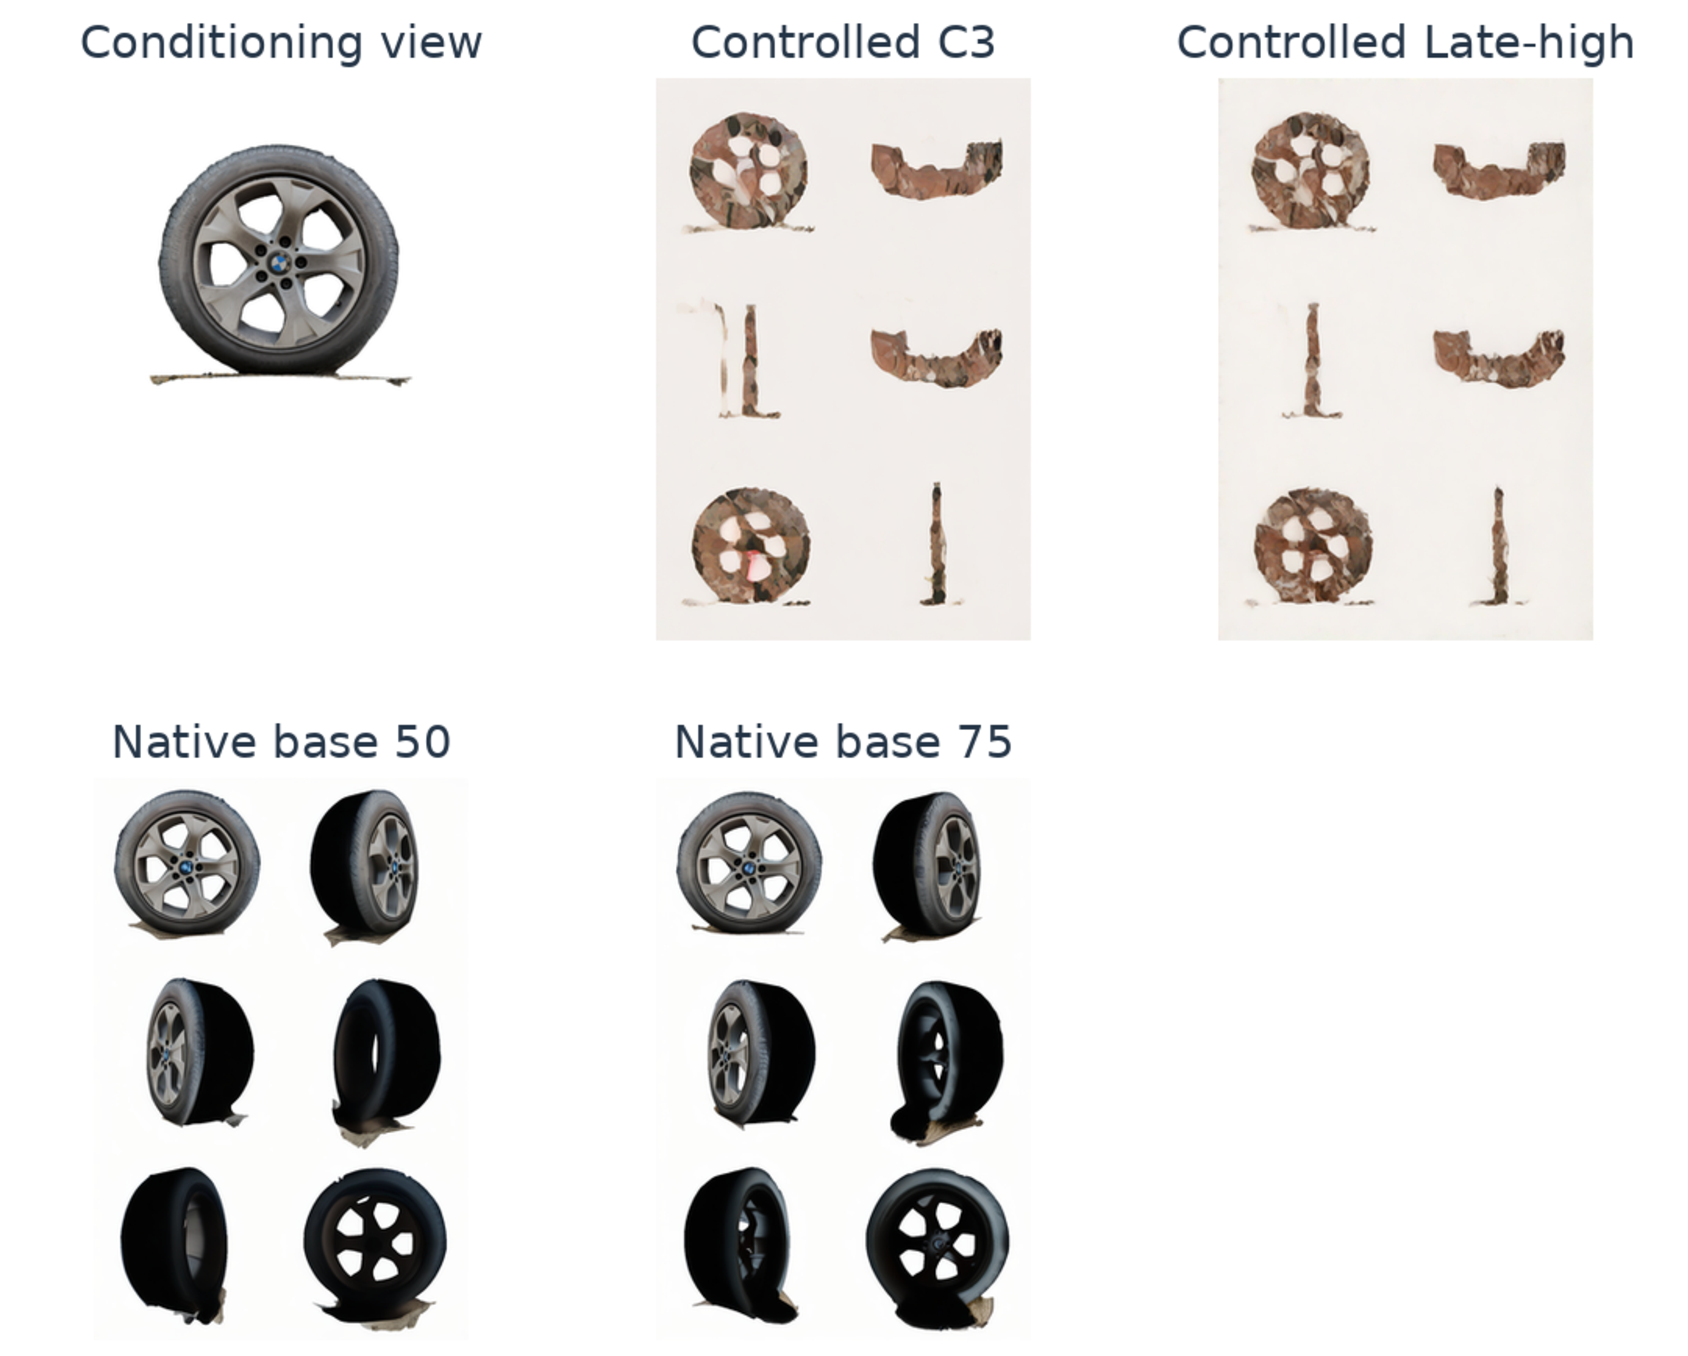
\includegraphics[width=\linewidth,height=0.72\textheight,keepaspectratio]{figures/figS_base_diagnostic014_02.pdf}
\caption{Retained complete grids for a fixed input-order failure object. The disabled-adapter visual column is omitted; its records remain available. Native base outputs use a different sampler and unverified camera conventions, so these are protocol diagnostics rather than aligned GT comparisons or complete default GeoTex results. No reference-fidelity inference follows from the better front-looking native color. Object 2 of two.}
\end{figure}


The diagnostic separates online/cached image features, classifier-free guidance and other sampling differences only within these previously observed inputs. It does not identify a single cause, establish a new algorithm, validate broad material fidelity or replace any earlier paired comparison. No inferential statistics or new acceptance probability are assigned to these two examples.

\subsection*{Controlled guidance--image-feature diagnostic}
\addcontentsline{toc}{subsection}{Controlled guidance--image-feature diagnostic}
The same two seen failure objects undergo eight calls: cached/online global image features crossed with conditional-only/sequential CFG2, all without geometry residuals. Views remain 256 pixels, the sampler remains the frozen 50-step EulerDiscreteScheduler, and conditioning RGB/initial latent identities match the old control. Online encoders consume the same already processed conditioning RGB; native RGBA recentering and bright-pixel handling are not invoked. The online-to-cache feature cosines are 0.862997 for LG Remote and 0.899210 for Tire. Feature difference is not itself a fidelity measure or evidence of a bad cache.

The conditional-only arms reuse the original generation function. The cached arm reproduces both prior No Adapter RGB outputs bitwise. CFG2 uses the standard prediction $2\epsilon_c-\epsilon_u$ through sequential batch-one forwards. Negative conditioning encodes a zero tensor in the normalized VAE input space, with seed424242; its reference-noise call uses an independent RNG fork at each step (seed100042 plus step). The positive branch retains the original randomness: all fifty positive-call CUDA RNG states match across four arms for each object. Each guided arm records fifty positive and fifty negative calls; each conditional-only arm records fifty positive calls. This controlled sequential implementation is not claimed pixel-equivalent to the native batched CFG API.

\begin{figure}[p]\centering
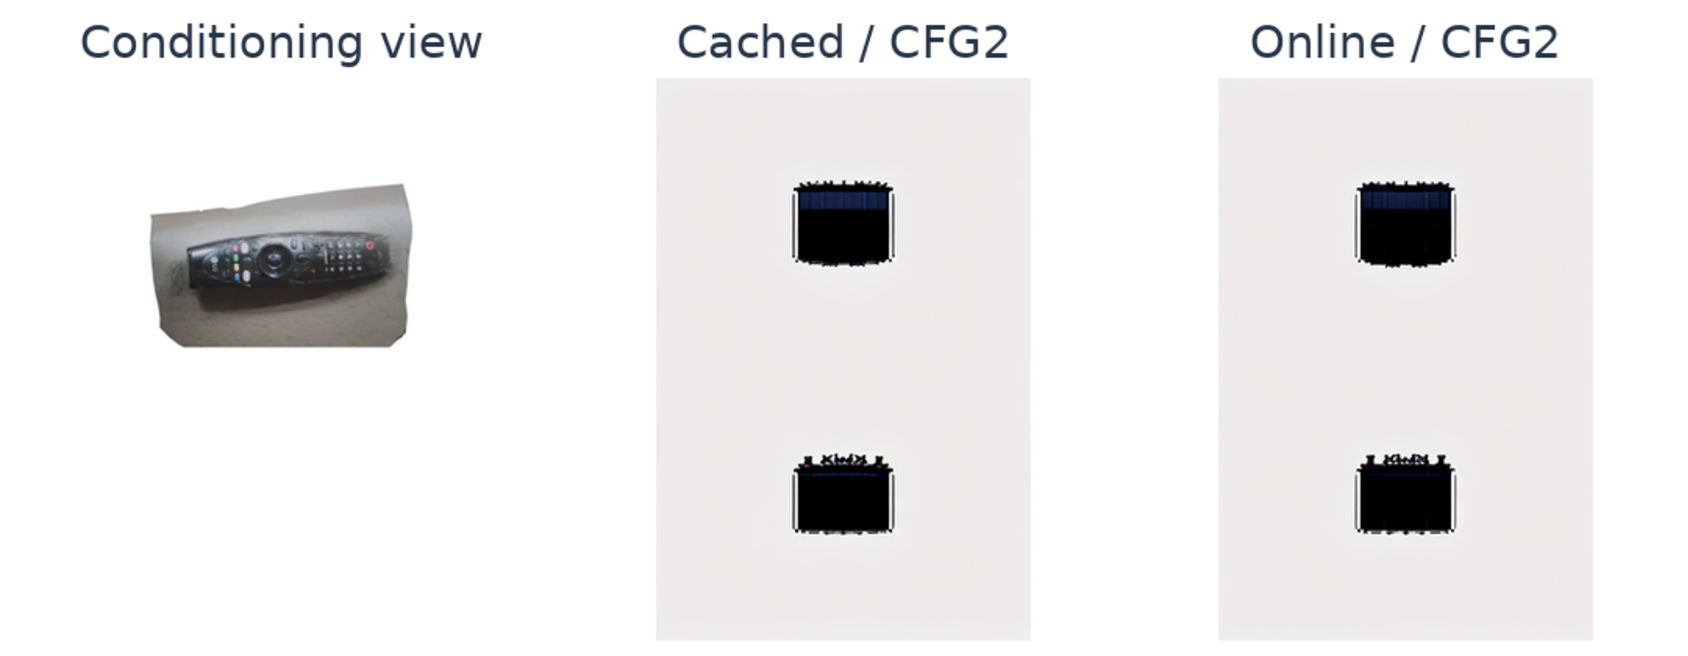
\includegraphics[width=\linewidth,height=0.72\textheight,keepaspectratio]{figures/figS_guidance_diagnostic014_01.pdf}
\caption{Guided cached/online-feature outputs for the fixed failure object. The two malformed unguided disabled-adapter columns are omitted from the display; all four original factorial arms and identity tests remain reported. Complete generated grids are resized only for presentation. The dark incorrect shapes remain, and online features do not establish a quality repair. These are previously inspected diagnostic examples, not a new holdout. Object 1 of two.}
\end{figure}

\begin{figure}[p]\centering
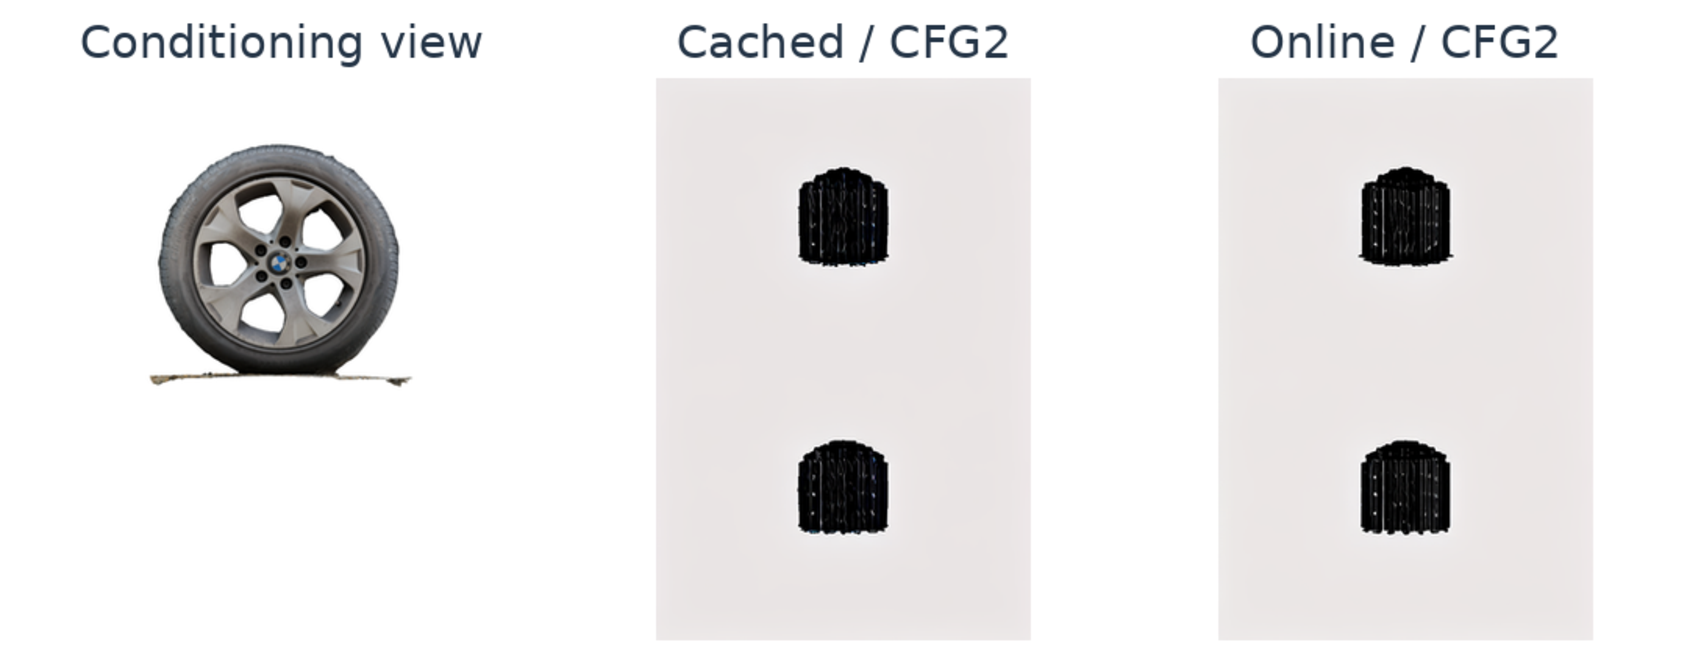
\includegraphics[width=\linewidth,height=0.72\textheight,keepaspectratio]{figures/figS_guidance_diagnostic014_02.pdf}
\caption{Guided cached/online-feature outputs for the fixed failure object. The two malformed unguided disabled-adapter columns are omitted from the display; all four original factorial arms and identity tests remain reported. Complete generated grids are resized only for presentation. The dark incorrect shapes remain, and online features do not establish a quality repair. These are previously inspected diagnostic examples, not a new holdout. Object 2 of two.}
\end{figure}


No paired cross-camera GT endpoints, population tests or acceptance probability are assigned to these two examples. The result retains the earlier B2 feature-substitution failure and C1 visual-gate failure; it does not support erasing those records or claiming a validated appearance correction. Resolution and remaining full-pipeline differences should be separated before deploying an amended GeoTex path or developing a new method.

\subsection*{Target-resolution bridge}
\addcontentsline{toc}{subsection}{Target-resolution bridge}
The two seen diagnostic objects undergo eight calls: 256/512-pixel target views crossed with conditional-only/sequential CFG2. Reference RGB resizing and model.img\_size remain 256; online global features, frozen model weights, 50-step EulerDiscrete sampling, training time IDs and reference encoding remain fixed. Initial latents have shape $1\times4\times96\times64$ or $1\times4\times192\times128$. Within each target resolution, the two arms use identical initial latents and fifty matching positive-call CUDA RNG states. Across resolutions, the tensor dimensions differ: a common seed is not a claim of identical initial tensors. Guided arms reuse the previous sequential CFG2 implementation and independent negative RNG policy.

Both 256-pixel arms reproduce the corresponding S6 online-feature RGB outputs bitwise for both objects. All conditions have identical reference-input and online-feature hashes within an object. Larger target grids change the object arrangement, but retained appearance defects prevent calling this a quality repair. Camera identities have not been independently calibrated across these generated grids, so there are no cross-path GT scores, population tests or deployment claims. The base pipeline source specifies a $1024\times1536$ output grid; this source fact and the controlled bridge motivate further protocol calibration, not retroactive pooling of different target resolutions.

\begin{figure}[p]\centering
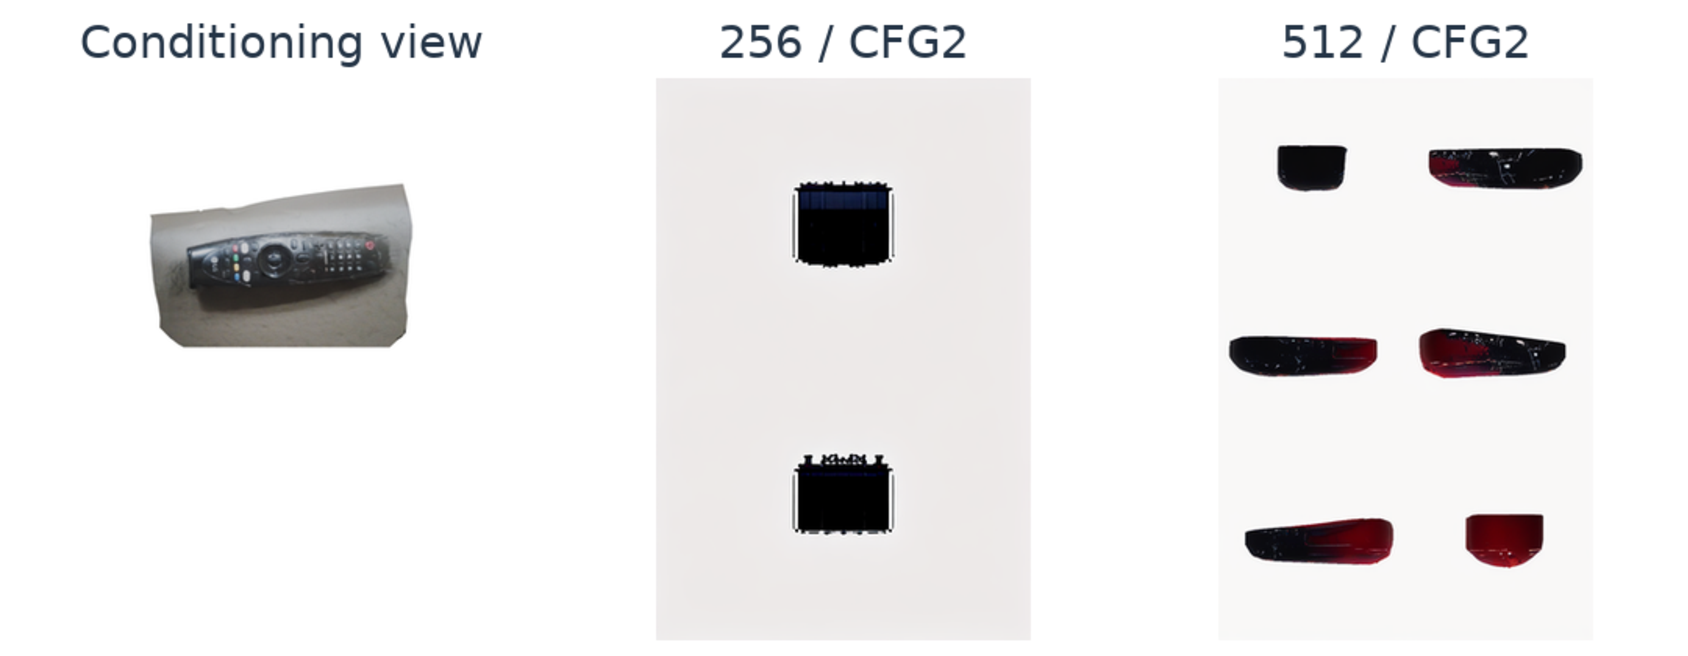
\includegraphics[width=\linewidth,height=0.72\textheight,keepaspectratio]{figures/figS_resolution_diagnostic014_01.pdf}
\caption{Guided 256/512-view outputs for the fixed failure object. Malformed unguided disabled-adapter columns are omitted; all original resolution arms remain in the protocol and numerical record. The complete grids preserve their contents. Camera identity has not been independently calibrated across target resolutions, so these are protocol/appearance diagnostics, not aligned GT comparisons or an established repair. Object 1 of two.}
\end{figure}

\begin{figure}[p]\centering
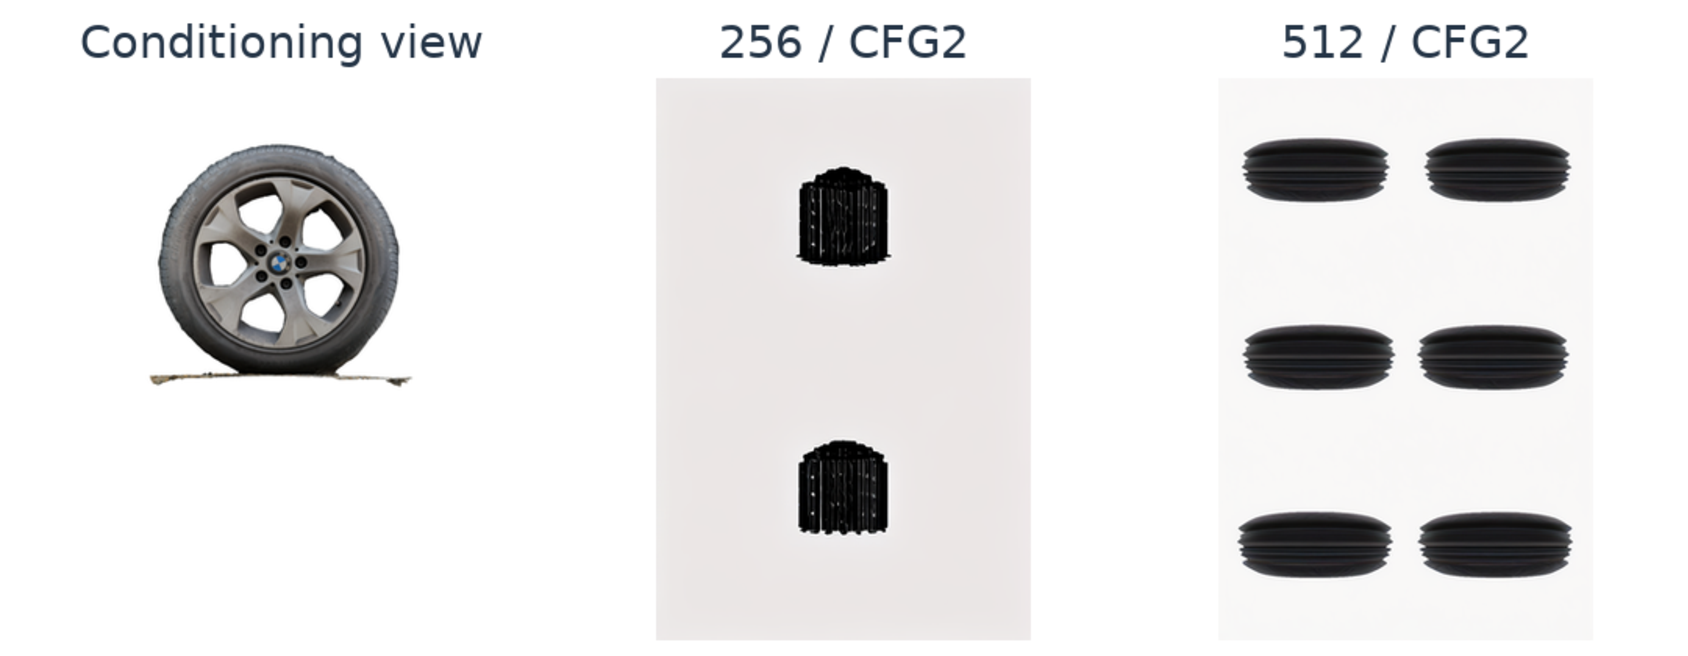
\includegraphics[width=\linewidth,height=0.72\textheight,keepaspectratio]{figures/figS_resolution_diagnostic014_02.pdf}
\caption{Guided 256/512-view outputs for the fixed failure object. Malformed unguided disabled-adapter columns are omitted; all original resolution arms remain in the protocol and numerical record. The complete grids preserve their contents. Camera identity has not been independently calibrated across target resolutions, so these are protocol/appearance diagnostics, not aligned GT comparisons or an established repair. Object 2 of two.}
\end{figure}


\subsection*{Native geometry implementation and camera-contract audit}
\addcontentsline{toc}{subsection}{Native geometry implementation and camera-contract audit}
The published inference source at commit \texttt{f714682db5e6f78e8d1c7c0a43d1525638dda5a6} arranges rendered indices $[0,5,1,4,2,3]$ in row-major order; its bake script extracts result tiles $[1,3,5,6,4,2]$, the inverse permutation. Actual metadata for all ten baking objects matches those nominal directions after the conditioning-camera anchor rotation. Pole elevation matches, but pole-image roll, cross-renderer pixel registration and generated-view fidelity remain unverified. The historical public training loader's repeated top view is separate from this inference contract. Source snapshots, hashes and the ten-object audit are provided.

Two seen objects first pass an identity gate: the frozen GeoTex weights are loaded, all geometry features cleared, and the full native pipeline outputs match the earlier bare-base RGB pixels exactly. The model constructor already wraps reference attention; setting its preparation state prevents double wrapping without replacing the native denoising loop.

The subsequent matrix has eight conditions per object: disabled, original unscaled residual, Fixed Low, Fixed High, Fixed Mean, C3, Late-high and Generic Linear. Native target views remain 512 pixels with CFG2 and fifty EulerAncestral steps; the trained geometry encoder input remains 256 pixels, with wrapper interpolation to actual hidden-state sizes. Historical schedule functions come from the frozen registry; Fixed Mean requests 1.65 and Late-high requests 1.25 except for the last sixteen steps at 2.50. Applied layer caps remain native. Historical C3's group-dependent profile does not share every layer budget with the scalar Fixed Mean; no equal-budget claim is made for that contrast.

Geometry features have batch one and broadcast to both batch-two CFG branches through hidden-state-dependent gates. All nine wrappers skip fifty reference-write corrections and execute fifty corrected read calls; each geometry-enabled correction has batch two and finite values. Within an object, geometry/input hashes, initial latents and the fifty outer-UNet CUDA RNG states match across all eight conditions. The disabled arm reproduces the previous bare native grid bitwise. The initial registry-import attempt failed before model loading because its required run configuration was absent; the failed source/record is retained, and the corrected attempt has a distinct output root.

\begin{figure}[p]\centering
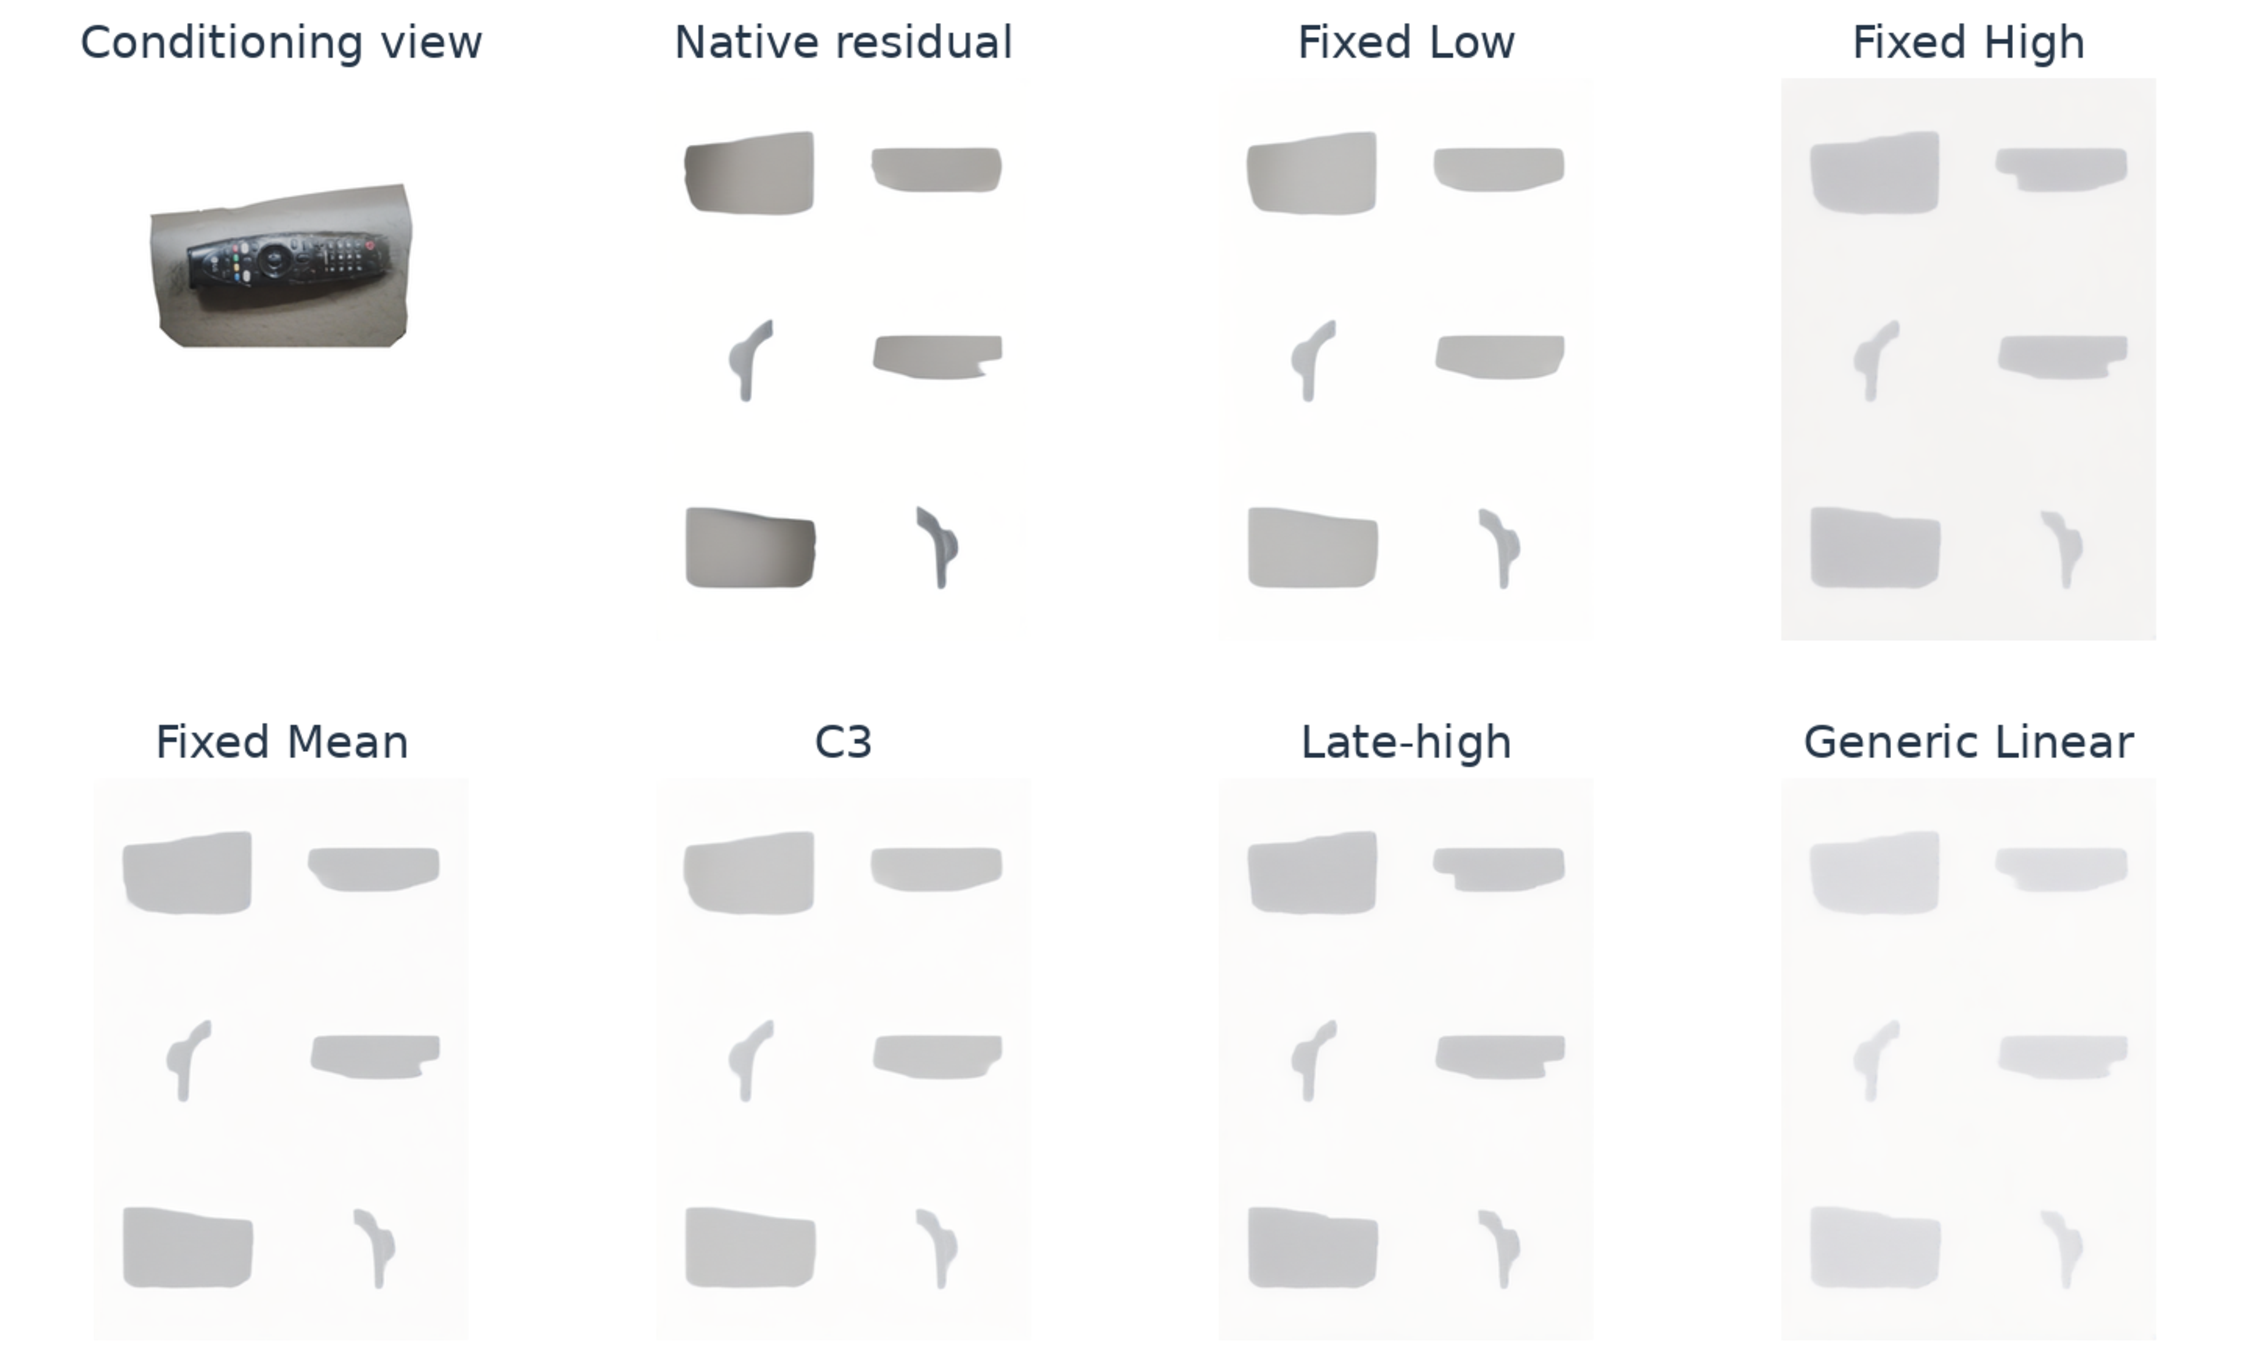
\includegraphics[width=\linewidth,height=0.72\textheight,keepaspectratio]{figures/figS_geometry_diagnostic014_01.pdf}
\caption{Retained complete native-loop geometry grids for a fixed input-order object. All seven enabled geometry settings are shown; the malformed disabled-adapter visual column is omitted, without changing any numerical results or failure records. Full-grid source pixels are preserved. The two input-order rights-cleared objects and their attribution remain the same; these observed outputs establish no general quality repair. Object 1 of two.}
\end{figure}

\begin{figure}[p]\centering
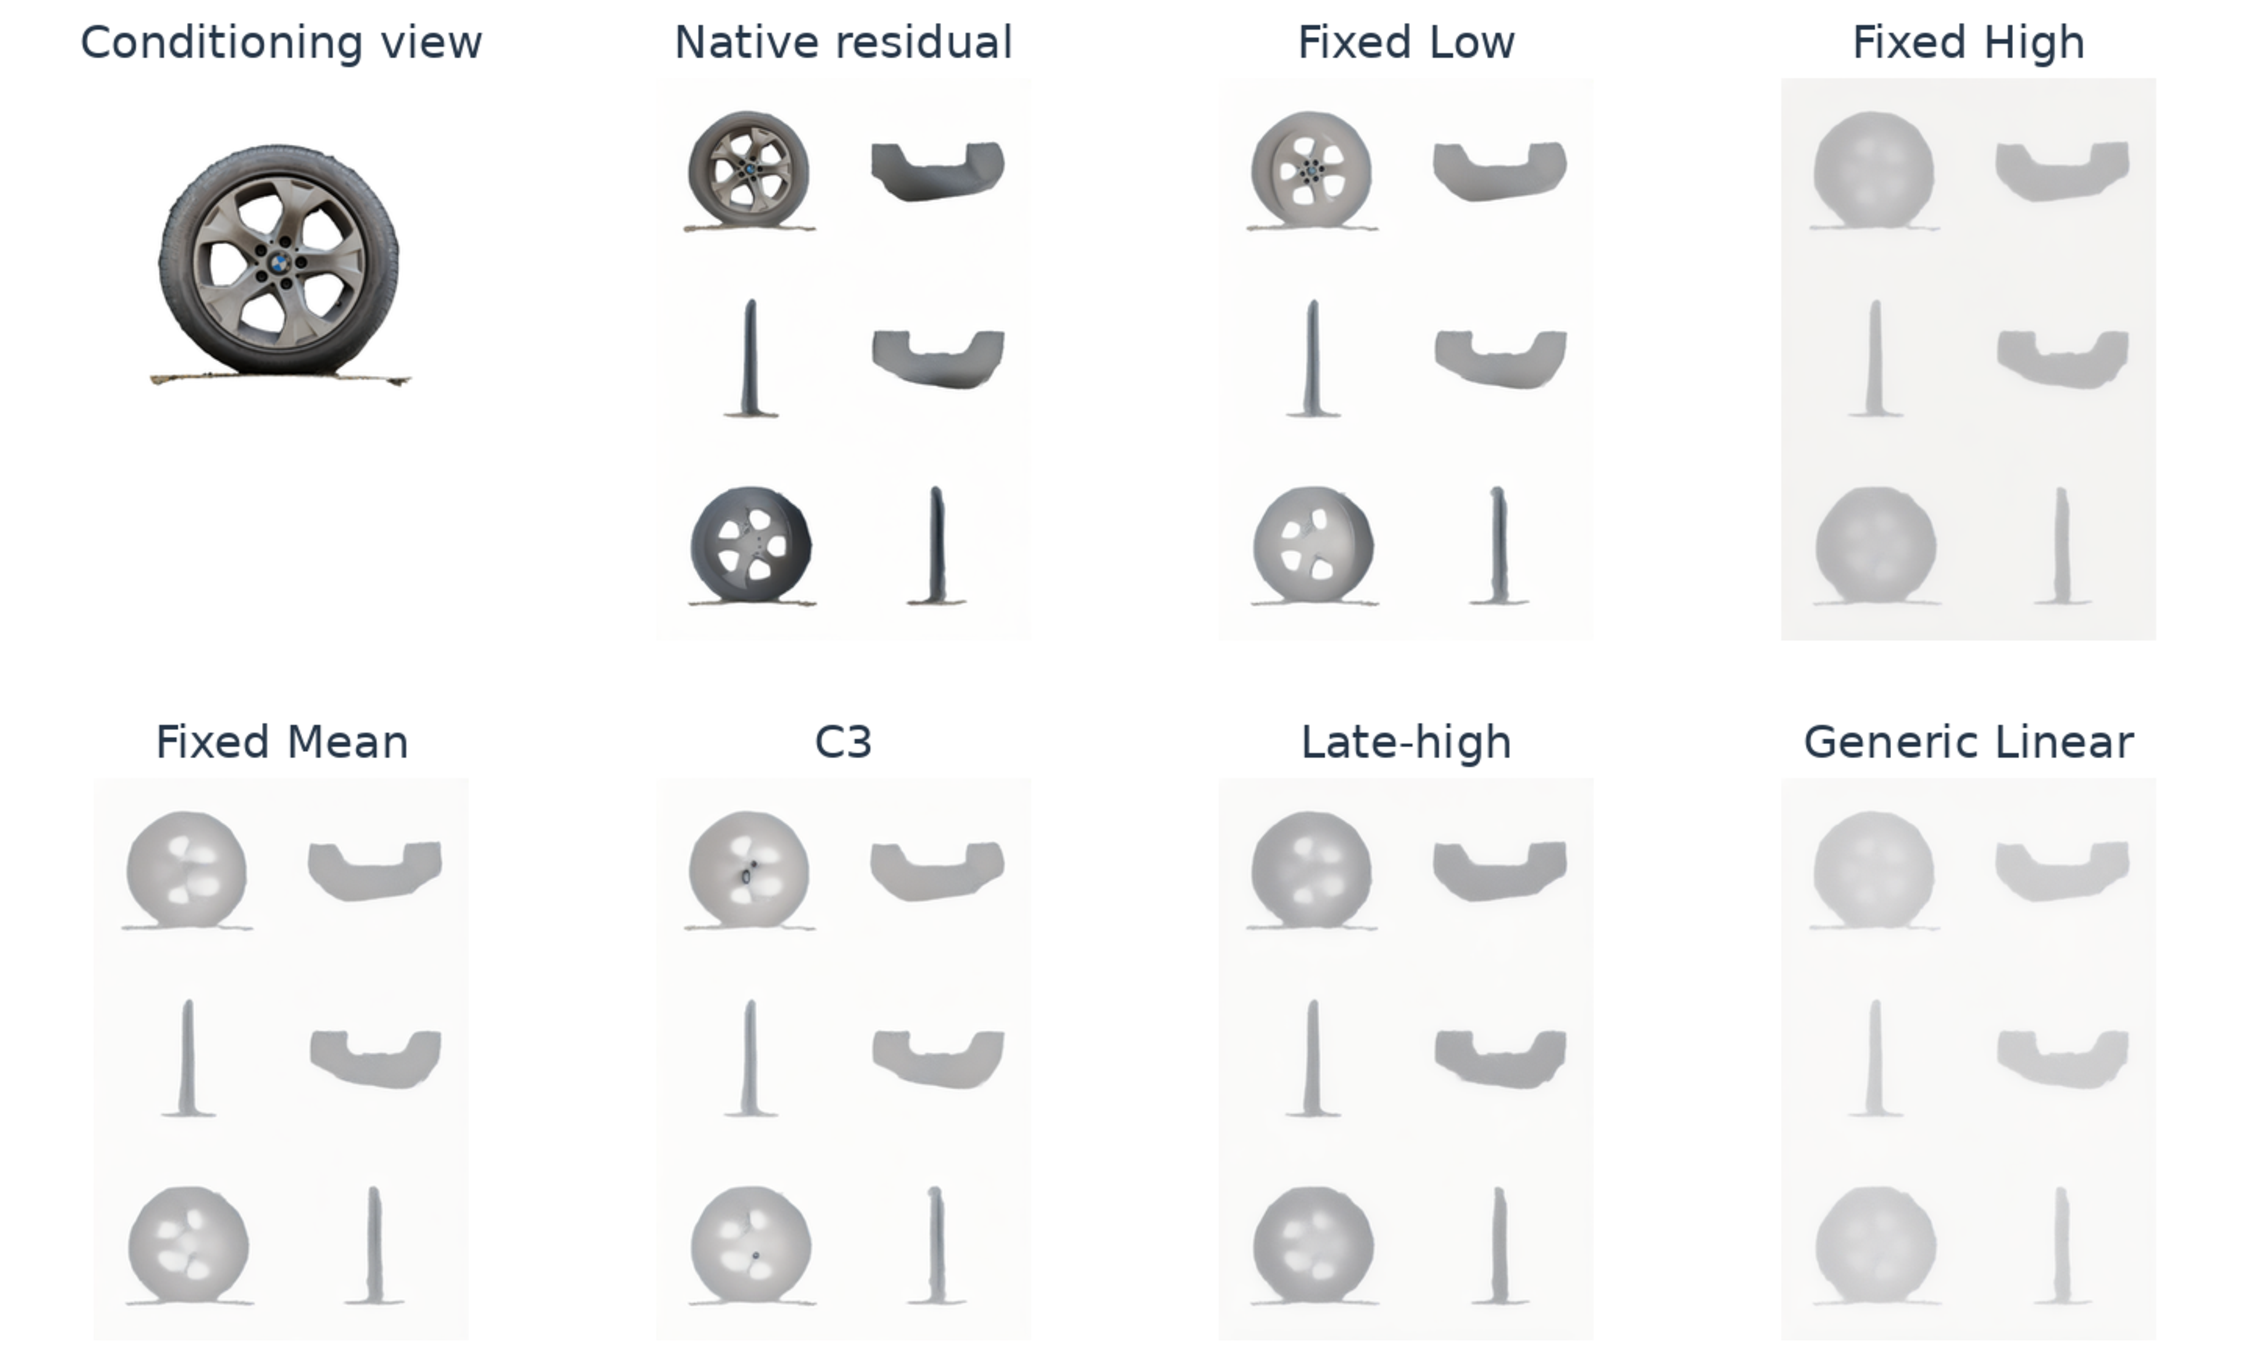
\includegraphics[width=\linewidth,height=0.72\textheight,keepaspectratio]{figures/figS_geometry_diagnostic014_02.pdf}
\caption{Retained complete native-loop geometry grids for a fixed input-order object. All seven enabled geometry settings are shown; the malformed disabled-adapter visual column is omitted, without changing any numerical results or failure records. Full-grid source pixels are preserved. The two input-order rights-cleared objects and their attribution remain the same; these observed outputs establish no general quality repair. Object 2 of two.}
\end{figure}


These diagnostics are not an independent confirmation cohort, do not verify correct generated cameras and do not support population inference or cross-path GT statistics. They preserve the prior controlled and downstream results while restricting claims about native deployment. Geometry-encoding resolution and CFG-branch compatibility require further controlled examination.

\subsection*{Geometry encoding, CFG branch policy and training-lineage limits}
\addcontentsline{toc}{subsection}{Geometry encoding, CFG branch policy and training-lineage limits}
The same two seen objects undergo twelve native-loop calls: geometry encoding at 256/512 pixels crossed with both-branch, conditional-only and conditional-only half-amplitude corrections. The native target grid, reference RGBA, online features, CFG2 and fifty EulerAncestral steps remain fixed. A controller acts after native correction computation: the both mode returns the correction unchanged; conditional-only zeros the negative sample; half-amplitude also multiplies the positive sample by 0.5. This is an implementation diagnostic, not a newly validated algorithm or a residual-dose-matched comparison. Half amplitude checks the conditional coefficient in CFG2; different trajectories prevent claiming equal total residual norms.

The 256/both output reproduces both S6 original-residual RGB grids bitwise. All nine wrappers retain fifty reference-write skips and fifty corrected reads. Input hashes, initial latents and outer-UNet RNG trajectories match within each object; geometry input/feature hashes match only within the same geometry encoding size. Every conditional-only read has zero negative correction norm. Complete output grids and trace identities are delivered.

\begin{figure}[htbp]\centering
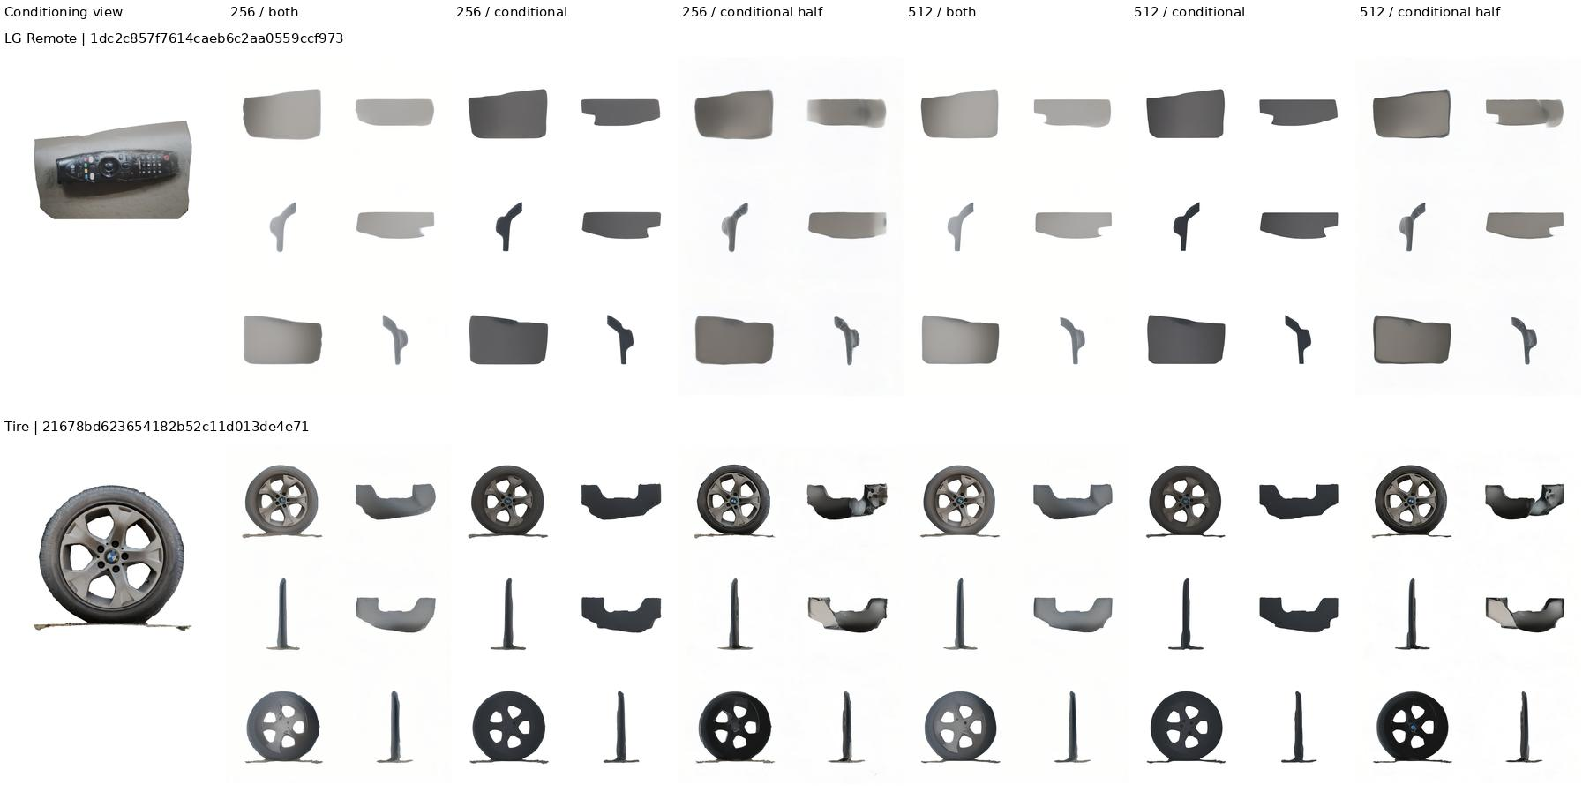
\includegraphics[width=\linewidth,height=0.74\textheight,keepaspectratio]{figures/figS8_encoding_branch_matrix.pdf}
\caption{All twelve full grids, resized only for display. Half-amplitude conditional corrections preserve more tire details, but remote reference content is still lost. Neither larger geometry encoding nor branch removal establishes an overall quality repair. Same previously inspected objects and attribution as S6.}
\end{figure}

The frozen checkpoint's recorded main-adapter training lineage includes a 1,118-object list, a matching checkpoint SHA256 and a complete 2,000-step loss CSV. The train list has no UID overlap with Fresh C; 1,112 objects have the six checked RGB/normal/depth input sets, and six have missing entries. These availability counts do not establish texture quality or authenticate each historical sampled object. The configuration specifies 256-pixel training and conditioning-drop probability 0.1, but the recorded custom training entry does not read that probability and uses only non-dropped conditioning. It bypasses the model-class training method. The historical dataset source has repeated-top target lists; the surviving dataset source differs from the recorded commit. Source and model-entry identities, the declared list override, checkpoint identity and current availability are audited separately.

Exact training replay remains unsupported: the transient list-override wrapper and training seed are not preserved, the CSV has no sampled-object identities, and the checkpoint contains adapter/encoder weights without an embedded step. A trailing literal newline escape in the original manifest is preserved and explicitly handled rather than silently rewriting that artifact. This audit concerns the current main-adapter lineage, not restoration of the historical FAC branch. Conditional-only training explains why unrestricted negative-branch insertion needs validation, but the controlled outputs do not establish it as the sole cause of appearance loss. No independent generalization or cross-camera GT inference is made.

\FloatBarrier
\section*{S7. Historical selection, preference and FAC records}
\label{supp:group7}
\addcontentsline{toc}{section}{S7. Historical selection, preference and FAC records}

\subsection*{Historical 01549 Table 9: strict-276 schedule transfer}
\addcontentsline{toc}{subsection}{Historical 01549 Table 9: strict-276 schedule transfer}
The 01549 submission reports this schedule-transfer comparison on the 276 objects disjoint from the 24-object probe. It uses the strong-residual, per-layer-capped v2 adapter, not the v1 checkpoint named for 01549 Table 4. The values below are reproduced from the authenticated 01549 submission; they are not pooled with Fresh C or the separate MAIN-STAGE-276 profile-placement analysis. The table therefore documents schedule transfer on its stated adapter instance and remains distinct from Fresh C's matched single-checkpoint comparison.

\begin{table}[ht]
\centering\small
\caption{Values reproduced from original 01549 Table 9 for the stated strict-276 retrospective schedule-transfer comparison. The adapter/run differs from Fresh C; row-level runner and input provenance are incomplete. Values are preserved as submitted historical results, not independently verified statistics.}
\label{tab:historical-table9}
\begin{tabular}{lcccc}
\toprule
Schedule & FG-SSIM & PSNR & C3--schedule $\Delta$PSNR (95\% CI) & C3-favourable objects \\
\midrule
Trapezoid & 0.356 & 19.04 & $+0.258$ $[+0.207,+0.308]$ & 206/276 \\
Gaussian peak & 0.358 & 18.97 & $+0.324$ $[+0.281,+0.367]$ & 232/276 \\
Linear warm-up & 0.377 & 18.97 & $+0.323$ $[+0.263,+0.386]$ & 214/276 \\
Cosine bump & 0.330 & 18.39 & $+0.902$ $[+0.824,+0.981]$ & 253/276 \\
C3 (TCAS) & 0.376 & 19.29 & -- & -- \\
\bottomrule
\end{tabular}
\end{table}

\subsection*{Historical 01549 Table 3: extended 24-object development diagnostics}
\addcontentsline{toc}{subsection}{Historical 01549 Table 3: extended 24-object development diagnostics}
The table below is transcribed from the authenticated 01549 source and moved from the main text to preserve the original 24-object development record. The candidate-level row outputs and selection-time provenance are unavailable for independent reanalysis. Laplacian variance, RGB standard deviation, gradient magnitude, and high-frequency energy are variation diagnostics; this historical table does not establish texture fidelity, a population effect, or an optimal schedule.

\begin{table}[ht]
\centering\small
\caption{Values transcribed from original 01549 Table 3 for representative variants in the 24-object development probe. These are historical values, not independently recomputed statistics; variation measures do not establish texture fidelity.}\label{tab:historical-table3}
\begin{tabular}{lcccc}
\toprule
Variant & $\Delta$Lap Var & $\Delta$RGB Std & $\Delta$Grad & $\Delta$HF Energy \\
\midrule
C3 & $-$0.001 & $-$0.023 & +0.142 & +0.058 \\
C4 & $-$0.012 & $-$0.032 & +0.086 & +0.062 \\
A\_s2.50 & $-$0.011 & $-$0.044 & +0.054 & +0.078 \\
A\_s2.00 & $-$0.006 & $-$0.040 & +0.100 & +0.070 \\
A\_s1.25 & $-$0.005 & $-$0.032 & +0.104 & +0.053 \\
\bottomrule
\end{tabular}
\end{table}

\clearpage
\subsection*{First-round FAC controlled re-examination}\label{supp:fac-historical}
\addcontentsline{toc}{subsection}{First-round FAC controlled re-examination}
The 01549 first-round package reports seven trained FAC configurations under the paired 300-object protocol. All values below are retained as originally reported; this is not a new 1008 training run. The separate 12-object untrained C3-envelope control is retained in the historical protocol paragraph below.

\begin{longtable}{p{3.3cm}p{3.5cm}rrrr}
\caption{FAC dose-response table reported in the first-round 01549 supplement. FG-PSNR and FG-SSIM are the reported absolute values; $\Delta$FG-PSNR and wins compare each trained configuration with TCAS.}\label{tab:fac-dose-response}\\
\toprule
Configuration & Temporal gate & FG-PSNR & FG-SSIM & $\Delta$FG-PSNR & Wins \\
\midrule\endfirsthead
\toprule
Configuration & Temporal gate & FG-PSNR & FG-SSIM & $\Delta$FG-PSNR & Wins \\
\midrule\endhead
TCAS baseline (C3) & fixed C3 & 9.88 & 0.3681 & -- & -- \\
LTAG only & joint, unconstrained & 7.79 & 0.3487 & $-2.08$ & 4/300 \\
LTAG+GSG & joint, unconstrained & 7.03 & 0.3163 & $-2.84$ & 6/300 \\
Full FAC & joint, unconstrained & 6.94 & 0.3204 & $-2.94$ & 5/300 \\
Two-stage + GSG/FSC & frozen at C3 & 7.32 & 0.3074 & $-2.56$ & 4/300 \\
Envelope penalty ($\lambda=1$) & joint, penalized to C3 & 7.14 & 0.3021 & $-2.74$ & 2/300 \\
Fidelity weighting & frozen at C3 & 7.51 & 0.3110 & $-2.37$ & 5/300 \\
Gentle schedule & frozen at C3 & 8.77 & 0.4175 & $-1.10$ & 48/300 \\
\bottomrule
\end{longtable}

The submitted protocol states that only the LTAG/GSG/FSC controllers (roughly $6\times10^3$ parameters) were trained; the base model, VAE, and GeoTex-Adapter remained frozen. It specifies the enhanced latent denoising objective and 2,000 AdamW steps on a training pool stated as 1,706 objects. The separate 12-object untrained control was reported at $\Delta$FG-PSNR $=-0.18$ dB (95\% CI [$-0.42,+0.05$]). A recovered configuration instead lists 1,200 training objects, and no run-bound seed/output manifest was found. We retain the original values as reported and disclose this reproducibility limit. Recoverable code is now supplied with the bounded source/component checks below; a complete historical training replay remains unverified.

\subsection*{Retrospective texture-complexity boundary}
\addcontentsline{toc}{subsection}{Retrospective texture-complexity boundary}
This analysis uses the separate FRESH\_CONFIRM\_300 cohort ($N=300$), not Fresh C or Fresh B. LLH and native GFL rows match the frozen object list and share the recorded checkpoint, runner, seed, six unique target views, sampler, and protocol. The paired LLH--GFL mean differences are $+1.2877$ dB FG-PSNR (95\% object-bootstrap CI [$+0.9383,+1.6346$]; 57.7\% LLH-favorable objects) and $-0.01650$ FG-LPIPS ([$-0.01887,-0.01413$]; 73.3\% LLH-favorable objects).

The descriptor analysis tests two image-space outcomes against five ground-truth descriptors: foreground Laplacian variance, RGB standard deviation, gradient magnitude, high-frequency energy, and coverage. Spearman correlations use average ranks and paired-object percentile bootstrap intervals (10,000 resamples, seed 20261002). The family contains ten plus-one-corrected bootstrap sign tests and Holm correction across all ten. Nine tests reject at 0.05; the only non-rejection is FG-LPIPS versus coverage (adjusted $p=0.0508$). The preserved H5 hypothesis excerpt predates one archived outcome bundle, but the main multiplicity lock classifies this family as retrospective after prior outcome exposure; that chronology has not been reconciled. We therefore report all associations as retrospective sensitivity evidence, not as preregistered confirmation.

\begin{table}[ht]
\centering\scriptsize
\caption{Retrospective Spearman associations between LLH--GFL image-space deltas and ground-truth descriptors in FRESH\_CONFIRM\_300. Correlation intervals are paired-object bootstrap intervals; adjusted $p$ values use the ten-test Holm family with plus-one-corrected bootstrap sign tests.}
\label{tab:texture-complexity}
\begin{tabular}{llrrl}
\toprule Outcome delta & Ground-truth descriptor & $\rho$ [95\% CI] & Holm $p$ & Decision \\
\midrule
FG-PSNR & Laplacian variance & $-0.524$ [$-0.603,-0.435$] & 0.0020 & reject \\
FG-PSNR & RGB standard deviation & $-0.380$ [$-0.488,-0.266$] & 0.0020 & reject \\
FG-PSNR & Gradient magnitude & $-0.464$ [$-0.548,-0.371$] & 0.0020 & reject \\
FG-PSNR & High-frequency energy & $-0.691$ [$-0.745,-0.626$] & 0.0020 & reject \\
FG-PSNR & Foreground coverage & $-0.134$ [$-0.241,-0.026$] & 0.0352 & reject \\
FG-LPIPS & Laplacian variance & $+0.604$ [$+0.511,+0.681$] & 0.0020 & reject \\
FG-LPIPS & RGB standard deviation & $+0.379$ [$+0.272,+0.482$] & 0.0020 & reject \\
FG-LPIPS & Gradient magnitude & $+0.563$ [$+0.469,+0.643$] & 0.0020 & reject \\
FG-LPIPS & High-frequency energy & $+0.677$ [$+0.599,+0.744$] & 0.0020 & reject \\
FG-LPIPS & Foreground coverage & $-0.118$ [$-0.233,+0.0002$] & 0.0508 & not rejected \\
\bottomrule
\end{tabular}
\end{table}

Ground-truth foreground Laplacian-variance quartiles contain 75 objects each. The FG-PSNR mean LLH--GFL difference declines from $+4.140$ dB in Q1 (92.0\% favor LLH) to $+1.127$ dB in Q2 (52.0\%), $-0.087$ dB in Q3 (41.3\%), and $-0.029$ dB in Q4 (45.3\%). The FG-LPIPS mean changes are $-0.03745$, $-0.01665$, $-0.00670$, and $-0.00520$ from Q1 to Q4; the favorable-object rates decline from 97.3\% to 50.7\%. These strata describe heterogeneity in this cohort. They do not establish that texture complexity causes the response, define a threshold, validate an object selector, or measure texture fidelity.

\clearpage

\subsection*{Retained original fixed-scale and C3 selection displays}
\addcontentsline{toc}{subsection}{Retained original fixed-scale and C3 selection displays}
These records retain their original classifications and limitations. Moving them changes presentation, not their outcomes or evidentiary status.

\subsection*{Historical Fixed-Scale Image-Space Diagnostics}
\addcontentsline{toc}{subsection}{Historical Fixed-Scale Image-Space Diagnostics}
\label{subsec:tradeoff}

Table~\ref{tab:sweep} reproduces the 13-scale sweep reported in the submitted 01549 manuscript. We retain it to preserve the original development question, but the object-level outputs, full run manifest, and metric implementation mapping are not available in the current authority. Its values and Figures~\ref{fig:curve}--\ref{fig:heatmap} are therefore historical diagnostics, not a new reanalysis or confirmatory evidence.

\begin{table}[t]
\centering
\caption{Historical 01549 report of a 13-scale sweep on the stated 50-object set. Values are reproduced from the submission and have not been independently recomputed from row-level outputs; they are retained as development diagnostics.}
\label{tab:sweep}
\small
\begin{tabular}{lcccc}
\toprule
Scale & $\Delta$FG-SSIM$\uparrow$ & POS & $\Delta$Crop-SSIM$\uparrow$ & $\Delta$PSNR$\uparrow$ \\
\midrule
0.75 & $-$0.013 & 20/50 & +0.113 & 7.53 \\
0.90 & +0.024 & 30/50 & +0.137 & 8.32 \\
1.00 & +0.047 & 34/50 & +0.147 & 8.79 \\
1.10 & +0.070 & 36/50 & +0.159 & 9.08 \\
1.15 & +0.071 & 36/50 & +0.157 & 9.25 \\
1.25 & +0.088 & 37/50 & +0.161 & 9.37 \\
1.35 & +0.100 & 39/50 & +0.163 & 9.63 \\
1.50 & +0.113 & 40/50 & +0.163 & 9.76 \\
1.60 & +0.120 & 42/50 & +0.166 & 9.83 \\
1.75 & +0.127 & 43/50 & +0.173 & 9.97 \\
2.00 & +0.134 & 44/50 & +0.169 & 9.96 \\
2.25 & +0.142 & 43/50 & +0.175 & 9.91 \\
2.50 & +0.145 & 44/50 & +0.165 & 9.91 \\
\bottomrule
\end{tabular}
\end{table}

The submitted table reports a rising $\Delta$FG-SSIM over most of the listed scale range and a near-plateau in the crop metric at higher settings. We retain this reported pattern only as historical motivation: absent row-level outputs and a complete run manifest, we do not treat it as an independently confirmed scale-response law. It motivates asking whether a single aggregate structural score fully describes the effect of adapter scaling.

\begin{figure}[t]
\centering
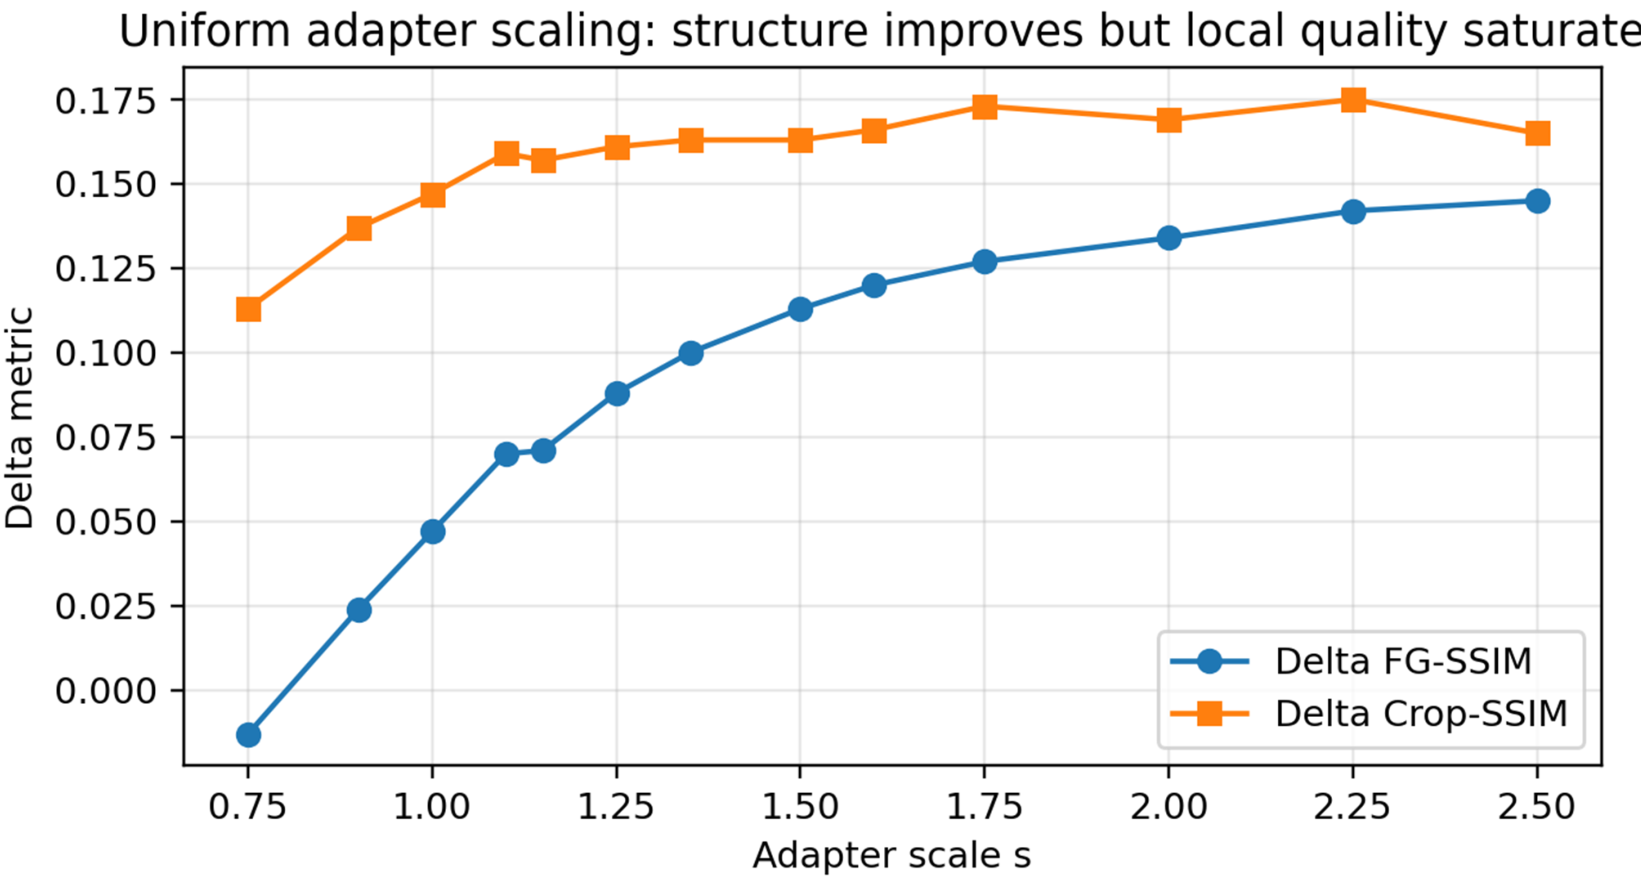
\includegraphics[width=\columnwidth]{fig2.pdf}
\caption{Historical fixed-scale diagnostic from the submitted 01549 paper. The plotted source reports FG-SSIM and Crop-SSIM over adapter scales; the underlying object-level run records are not available for independent reanalysis. It motivates measuring more than one endpoint, but is not a current confirmatory result.}
\label{fig:curve}
\end{figure}

The submitted heatmap depicts object-level variation across the reported scales, but its underlying rows cannot be reconstructed from the current evidence archive. We retain the visual diagnostic as part of the 01549 research history and do not infer a population-level response distribution from it. The updated Fresh C analysis below uses its own frozen cohort and matched inputs.

\begin{figure}[t]
\centering
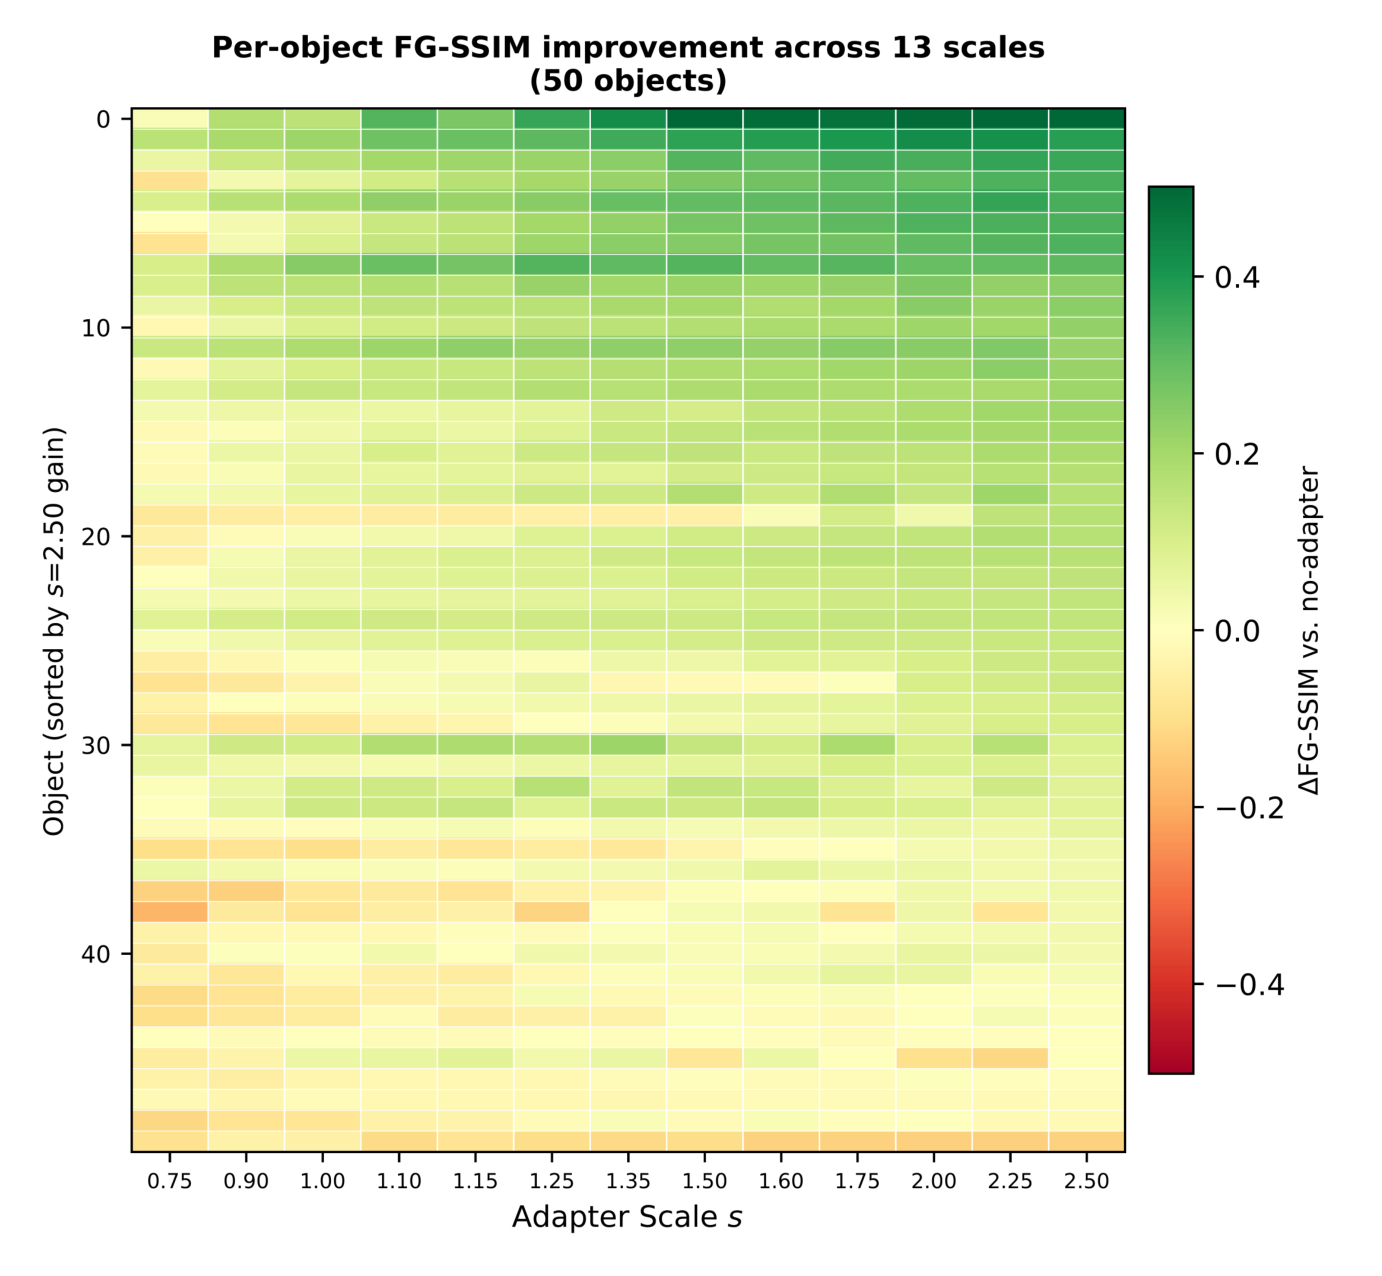
\includegraphics[width=\columnwidth]{fig3.pdf}
\caption{Historical per-object $\Delta$FG-SSIM heatmap reproduced from the 01549 submission (50 objects, 13 scales). The plot illustrates the originally reported response variation; row-level provenance is incomplete, so it is not used for a current population inference.}
\label{fig:heatmap}
\end{figure}

\subsection*{C3 Development Record and Current Evaluation}
\addcontentsline{toc}{subsection}{C3 Development Record and Current Evaluation}
\label{subsec:c3}

The submitted paper records 17 uniform, layer-wise, and timestep-conditioned variants on a 24-object development probe and identifies C3 as its chosen profile. This study question remains relevant: does a stage-dependent request offer a useful control setting beyond a single global scale? Because the complete historical row-level data and selection provenance are not available in the current authority, the original Table~\ref{tab:probe} and Figure~\ref{fig:pareto} are retained as historical development records, not as a verified ranking or proof of optimality. Fresh C evaluates the recorded C3 profile without another schedule search.

\begin{table}[t]
\centering
\caption{Representative values reported for the historical 24-object, 17-variant development probe. The full candidate set is shown in Figure~\ref{fig:pareto}. The underlying row-level outputs and selection-time provenance are not available for independent reanalysis; the table records the submitted development result and does not establish an optimum.}
\label{tab:probe}
\footnotesize\setlength{\tabcolsep}{3pt}
\begin{tabular}{llcc}
\toprule
Variant & Reported category & $\Delta$FG-SSIM & $\Delta$Lap Var \\
\midrule
C4 & Late-stage high & 0.105 & $-$0.0120 \\
C2 & Timestep schedule & 0.104 & $-$0.0110 \\
B2 & Layer-wise schedule & 0.090 & $-$0.0135 \\
A\_s2.00 & Uniform & 0.087 & $-$0.0062 \\
C3 & Mid-stage high & 0.084 & $-$0.0006 \\
A\_s2.25 & Uniform & 0.079 & $-$0.0096 \\
A\_s2.50 & Uniform & 0.078 & $-$0.0108 \\
B6 & Layer-wise schedule & 0.000 & $-$0.0027 \\
\bottomrule
\end{tabular}
\end{table}

The original table and plot use shape and texture-variation proxies to describe the development choice. They do not establish that texture was faithful to the reference, nor that C3 was the unique best candidate. In this revision, C3 is therefore described as the historical profile carried forward for matched evaluation, not as a theorem-derived or globally optimal schedule.

The requested profile is piecewise constant over normalized sampling progress $p$:
\begin{equation}
s_{\mathrm{req}}(p) =
\begin{cases}
1.25, & 0 \le p < 1/3,\\
2.50, & 1/3 \le p < 2/3,\\
1.25, & 2/3 \le p \le 1,
\end{cases}
\qquad \mathrm{C3}=(1.25,2.50,1.25).
\end{equation}
This is an inference-time instruction on the existing adapter path; no weights are trained. Its tested value is task- and implementation-specific. The schedule operation itself is not claimed as a new general primitive.

\begin{figure*}[!t]
\centering
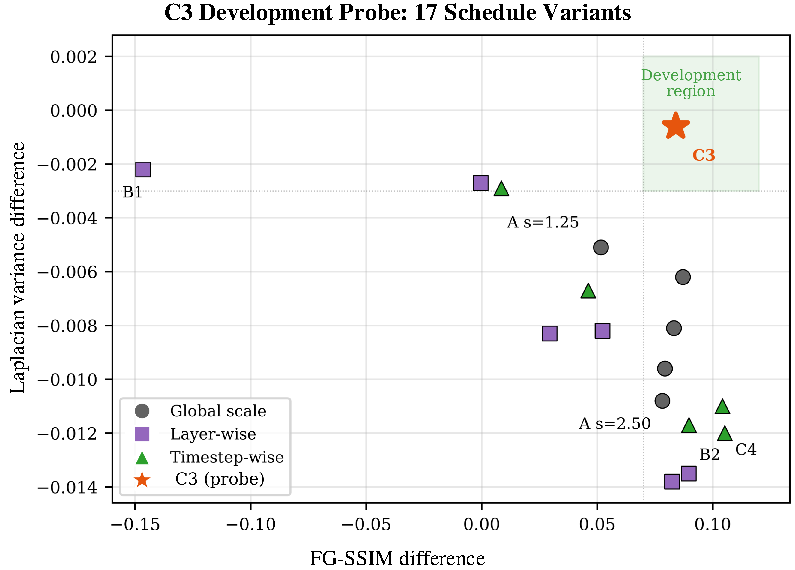
\includegraphics[width=0.78\textwidth]{figures/fig7_c3_development.pdf}
\caption{Historical 17-variant development probe from the submitted 01549 paper (24 objects). The axes show changes in FG-SSIM and Laplacian variance; variance is a texture-variation diagnostic, not a fidelity measure. “C3” identifies the selected historical profile, not an optimum or general schedule law. The candidate-level outputs are unavailable for independent reanalysis.}
\label{fig:pareto}
\end{figure*}

The source Figure~5 (26-object texture ratios) is not included as an active result because its object IDs, selection trace, and metric lineage are incomplete. The original 24-object Table~3 is moved to Supplementary Section~S7 as a verbatim historical diagnostic, with no texture-fidelity or population inference. Both source assets remain preserved in the authenticated submission and forensic archive; neither decision removes the fixed-scale research question or the development record of C3.

\subsection*{Historical cluster-aware preference study}
\addcontentsline{toc}{subsection}{Historical cluster-aware preference study}
\label{subsec:preference}

The 01549 first-round revision reported a blinded three-alternative forced-choice study on 30 objects with 24 participants. Participants compared conservative fixed-scale, aggressive fixed-scale, and C3 outputs for texture naturalness, shape consistency, and overall quality; condition order was randomized per trial. Each criterion had 720 first-choice decisions. Table~\ref{tab:preference} reports the aggregate counts; participant-level responses are not redistributed with this revision.

\begin{table}[t]
\centering\scriptsize
\caption{First-round 01549 3AFC results retained as reported. Percentages use 720 decisions per criterion; preference is not a measure of reference texture fidelity.}
\label{tab:preference}
\setlength{\tabcolsep}{3pt}
\begin{tabular}{lccc}
\toprule
Method & Texture naturalness & Shape consistency & Overall quality \\
\midrule
$s=1.25$ & 332/720 (46.1\%) & 96/720 (13.3\%) & 176/720 (24.4\%) \\
$s=2.50$ & 104/720 (14.4\%) & 331/720 (46.0\%) & 126/720 (17.5\%) \\
C3 (TCAS) & 284/720 (39.4\%) & 293/720 (40.7\%) & 418/720 (58.1\%) \\
\bottomrule
\end{tabular}
\end{table}

The reported analysis used a two-level participant/object bootstrap with 10,000 resamples. C3's overall-quality share was 58.1\% (95\% CI [50.1\%, 65.8\%]); its differences from the conservative and aggressive baselines were +33.6 points (CI [19.3, 47.2]) and +40.6 points (CI [29.4, 51.8]). The single-criterion advantages for texture naturalness and shape consistency had intervals crossing zero. This bounded preference result does not validate texture fidelity, unseen-view quality, or the Fresh C cohort.

This minimal-risk, non-interventional study did not require formal ethics review or written informed consent under applicable local regulations and institutional requirements. Participants were informed about the study and provided oral consent. The study involved no intervention, sensitive personal information, biological samples, or participant safety risk.

\FloatBarrier
\subsection*{Recoverable FAC code and bounded component validation}
\addcontentsline{toc}{subsection}{Recoverable FAC code and bounded component validation}
The separate recovered-source archive supplies byte-preserved controller, training/evaluation entries, local source dependencies and configuration snapshots, with a per-file source/hash manifest. It distinguishes an earlier entry whose default also optimizes the base adapter/geometry encoder unless \texttt{--freeze\_adapter} is used, from the later controller-only entry that freezes these modules. Both remain unbound to the historical reported run; filenames and their existence cannot establish which complete CLI, weights and sampling order produced the old table.

Three distinct standalone CPU controller fixtures pass finite forward/gradient-path and bitwise state-save/load checks. The two recovered entries share byte-identical controller source; duplicate copies are not counted as independent validation. For nine adapters with 64-channel geometry and the delivered defaults, LTAG, LTAG+GSG and full FAC contain 3,433, 4,018 and 6,322 parameters. These tests exercise one injection point with synthetic 16-by-16 tensors, without a diffusion model, base weights or data. They validate component execution, not full-model training, old experiment identity or quality. The archived FSC actually uses real FFT rather than the DCT named in comments; its initial mask attenuates the test tensor and is not an exact identity. Current claims follow executable operations, not archival comments.

The supplied recovered 1,200-object configuration, missing historical seed/checkpoint and 1,706-object discrepancy remain unresolved. We provide code and an offline component rerun command, while explicitly withholding a complete historical FAC replay claim. The already reported FAC negative results are not reclassified as newly confirmed measurements.

\subsection*{Local historical weights and the original-cohort retraining addendum}\label{supp:original276-retrain}
\addcontentsline{toc}{subsection}{Local historical weights and the original-cohort retraining addendum}
Three existing files named \path{geotex_v2_ema_final.pt} independently match the previously recorded MD5 \texttt{a74cc1d16cb473a95022bdcbc58e1b22}. They are archive copies of the same historical v2 artifact, not three independent models. The submitted paper identifies v2 for the separate strong-residual Section 4.7/Table 9 and FAC context. Its main-table v1 file, \path{geotex_refattn_v1/geotex_step_0002000.pt}, lacks a recoverable run-bound byte identity. Consequently v2 recovery closes a v2 artifact-location question but not exact original-main-adapter replication.

The 12 October 2026 retraining removes all 79 intersections between the recorded 1,118 training UIDs and the historical 276 evaluation UIDs, retaining 1,039 training UIDs. The held-out list is exactly positions 24--299 of the original evaluation list; its recorded training intersection is zero. Training completes 2,000 steps with explicit seed 20261012 and the new step-2000 checkpoint SHA-256 \texttt{19ae8afa08886f774c1b18e1888badbc47108f820774906cd875a5aaa33cf05c}. This is one newly seeded checkpoint, not a measurement of training-seed variance. Evaluations retain No Adapter, Fixed Low 1.25, Fixed High 2.50 and C3, 50 Euler steps, 256-pixel target tiles and views [0,15,12,16,13,14]. Current audited source seeds data preprocessing with $42+\mathrm{index}$ and shared initial latents/inference with 42; conditions share one loaded batch and the same latent tensor. The resulting metrics use one $3\times2$ composite, not six independent statistical units.

The preserved full-frame metric uses all pixels. FG-PSNR uses pixels above the recorded foreground threshold; the audited mask-aware SSIM includes its documented local-mask dilation and the archived LPIPS masks normalized image inputs. These inherited definitions are not canonical interchangeable measures across interfaces. White-background PSNR replaces background pixels using the common target mask; its C3--Fixed High difference is $-1.313536$ dB, matching the foreground direction. No background-region metric is used to select a winning schedule. The endpoint reversal does not identify a new mechanism or validate physical material quality.

All 1,104 rows are unique and form a 276-by-four requested-slot Cartesian matrix; ordered \path{obj_0000} through \path{obj_0275} rows map to the evaluation manifest's requested list. The evaluation log records an empty-input error and a \path{wrong path} diagnostic for UID \path{f7ef602b19214debb0b350db9af55ff2}, requested index 46. The inherited loader catches this error and randomly substitutes another input without returning the actual UID. The manifest lacks actual loaded-UID/input hashes. Consequently exact 276-UID coverage, actual training--evaluation disjointness and the unique-object count cannot be certified. Each slot still shares one loaded batch across its four conditions, supporting bounded within-slot comparisons. Excluding \path{obj_0046} is an input-failure sensitivity rather than filtering by output quality: C3--Fixed High means over the remaining 275 requested slots are full-frame PSNR $+1.696532$ dB, FG-PSNR $-1.311046$ dB and FG-LPIPS $+0.011272$. All 276 original slots remain archived. Present-day helper-source snapshots are audited source rather than execution-time hashes; training-source/checkpoint hashes are checked against the preserved run manifest. The research-decision cohort was previously exposed and the analysis is retrospective.

The archived statistical audit resamples the 276 requested slots (10,000 bootstrap draws; 200,000 two-sided plus-one sign-flip draws), with a post-inspection 24-test Holm family covering eight endpoints and C3 against three controls. Because actual unique-object coverage is uncertified, these pointwise intervals and $p$ values are technical diagnostics, not validated independent-object confirmation. Complete positive, non-detected and negative results are retained in Table~\ref{tab:supp-original276}. No actual sampling overlap is inferred for the unauthenticated historical v1 weights merely from a later list intersection. Fixed Mean, early/late allocations and Generic Linear are absent; the matrix does not identify timing-only effects. Records, failure-log excerpt, ordinal-exclusion sensitivity and recomputation are in \path{data/original276_retrain}.

\begingroup\scriptsize
\begin{longtable}{p{3.0cm}p{2.7cm}p{5.0cm}lr}
\caption{Complete exploratory C3 paired contrasts in the retrained historical-request panel. A minus B; positive PSNR/SSIM and negative LPIPS favor C3. All 276 requested slots retained, including one unknown actual-UID substitution. Pointwise slot-bootstrap intervals, favorable-slot counts and diagnostic 24-test Holm $p$ are not independent-object confirmation.}\label{tab:supp-original276}\\
\toprule Contrast & Endpoint & Mean [95\% CI] & Favorable & Holm $p$ \\
\midrule\endfirsthead
\toprule Contrast & Endpoint & Mean [95\% CI] & Favorable & Holm $p$ \\
\midrule\endhead
C3 -- Fixed Low & Full-frame PSNR & $+0.40246\ [+0.32938,+0.47580]$ & 208/276 & 0.00012 \\
C3 -- Fixed High & Full-frame PSNR & $+1.69908\ [+1.62148,+1.77602]$ & 276/276 & 0.00012 \\
C3 -- No Adapter & Full-frame PSNR & $+6.12787\ [+5.94191,+6.31562]$ & 276/276 & 0.00012 \\
C3 -- Fixed Low & Full-frame SSIM & $+0.00218\ [+0.00158,+0.00278]$ & 178/276 & 0.00012 \\
C3 -- Fixed High & Full-frame SSIM & $+0.00646\ [+0.00564,+0.00727]$ & 231/276 & 0.00012 \\
C3 -- No Adapter & Full-frame SSIM & $+0.10147\ [+0.09752,+0.10532]$ & 276/276 & 0.00012 \\
C3 -- Fixed Low & Full-frame LPIPS & $+0.00437\ [+0.00364,+0.00511]$ & 43/276 & 0.00012 \\
C3 -- Fixed High & Full-frame LPIPS & $-0.00698\ [-0.00818,-0.00576]$ & 210/276 & 0.00012 \\
C3 -- No Adapter & Full-frame LPIPS & $-0.39728\ [-0.40313,-0.39148]$ & 276/276 & 0.00012 \\
C3 -- Fixed Low & FG-PSNR & $+0.78262\ [+0.69539,+0.86682]$ & 240/276 & 0.00012 \\
C3 -- Fixed High & FG-PSNR & $-1.31354\ [-1.38483,-1.24106]$ & 9/276 & 0.00012 \\
C3 -- No Adapter & FG-PSNR & $+2.62856\ [+2.24209,+3.01227]$ & 215/276 & 0.00012 \\
C3 -- Fixed Low & FG-SSIM & $+0.02074\ [+0.01823,+0.02336]$ & 237/276 & 0.00012 \\
C3 -- Fixed High & FG-SSIM & $-0.05961\ [-0.06303,-0.05605]$ & 9/276 & 0.00012 \\
C3 -- No Adapter & FG-SSIM & $-0.11892\ [-0.13162,-0.10631]$ & 44/276 & 0.00012 \\
C3 -- Fixed Low & FG-LPIPS & $-0.00048\ [-0.00106,+0.00012]$ & 174/276 & 0.11689 \\
C3 -- Fixed High & FG-LPIPS & $+0.01127\ [+0.01022,+0.01233]$ & 30/276 & 0.00012 \\
C3 -- No Adapter & FG-LPIPS & $-0.02180\ [-0.02572,-0.01789]$ & 217/276 & 0.00012 \\
C3 -- Fixed Low & Edge-SSIM & $+0.00717\ [+0.00626,+0.00810]$ & 236/276 & 0.00012 \\
C3 -- Fixed High & Edge-SSIM & $-0.02777\ [-0.02937,-0.02613]$ & 5/276 & 0.00012 \\
C3 -- No Adapter & Edge-SSIM & $+0.02619\ [+0.02167,+0.03055]$ & 213/276 & 0.00012 \\
C3 -- Fixed Low & White-background PSNR & $+0.78262\ [+0.69539,+0.86682]$ & 240/276 & 0.00012 \\
C3 -- Fixed High & White-background PSNR & $-1.31354\ [-1.38483,-1.24106]$ & 9/276 & 0.00012 \\
C3 -- No Adapter & White-background PSNR & $+2.62856\ [+2.24208,+3.01226]$ & 215/276 & 0.00012 \\

\bottomrule
\end{longtable}
\endgroup

\begin{table}[ht]
\centering\small
\caption{Historical-request condition means over 276 requested slots. One unknown actual UID was substituted; means are technical slot summaries, not independent-object estimates. Paired contrasts and their diagnostics are in Table~\ref{tab:supp-original276}.}
\label{tab:supp-original276-means}
\begin{tabular}{lrrrrr}
\toprule
Condition & Full PSNR & FG-PSNR & FG-LPIPS & FG-SSIM & Edge-SSIM \\
\midrule
No Adapter & 9.900 & 7.072 & 0.21750 & 0.39294 & 0.43594 \\
Fixed Low & 15.626 & 8.918 & 0.19618 & 0.25328 & 0.45496 \\
Fixed High & 14.329 & 11.014 & 0.18443 & 0.33363 & 0.48990 \\
C3 & 16.028 & 9.701 & 0.19570 & 0.27402 & 0.46213 \\
\bottomrule
\end{tabular}
\end{table}

\begin{figure}[ht]
\centering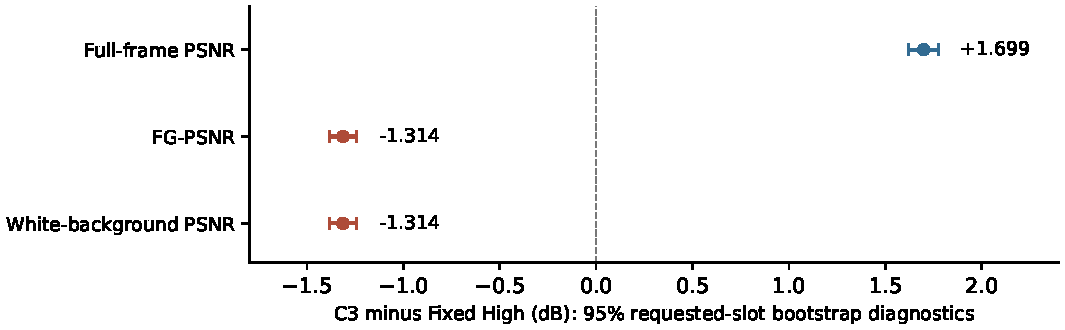
\includegraphics[width=0.88\textwidth]{figures/fig_original276_endpoint_sensitivity.pdf}
\caption{C3--Fixed High PSNR endpoint sensitivity in the retrained historical-request panel. Measurements use the same 276 requested slots, including one unknown replacement UID. Technical slot-bootstrap intervals do not validate independent-object replication. Excluding the recorded failed slot retains the opposing directions. The plot is computed from preserved CSV rows; no generated image is modified.}
\end{figure}

\FloatBarrier
\section*{S8. Auxiliary training, deployment and projection exploration}
\label{supp:group8}
\addcontentsline{toc}{section}{S8. Auxiliary training, deployment and projection exploration}

\subsection*{Native training inputs, numerical safeguards and fixed training protocol}
\addcontentsline{toc}{subsection}{Native training inputs, numerical safeguards and fixed training protocol}
The recorded custom trainer's shortcomings motivate a new main-adapter training protocol; this is not a FAC retraining or a replay of the historical pooled result. Of 1118 recorded training UIDs, six lack required inputs. Strict evaluation of the remaining 1112 retains 1090 and lists 22 input failures before any output-quality assessment. The old loader's random replacement of a failed object is disabled. The retained cohort has zero UID overlap with the 300 Fresh C objects. Geometry and target views are 512 pixels, use unique6 ordering, and have fixed resize ratio 1.0. Native reference preprocessing is captured from the actual pipeline at its first UNet call, including positive and negative CLIP embeddings, reference latents and added time IDs; these cached inputs are not generated evaluation outputs.

Three zero-valued depth channels in a real training object formerly produced a non-finite inverse-depth normalization. Values that cannot be inverted are encoded using the existing invalid-depth value before inversion; source RGB and normal maps are unchanged. This guard does not establish the physical meaning of those zero values. A separate precision probe finds all nine initial residual tensors nonzero, but their half-precision mean squares underflow to zero; float32 evaluation gives positive means of order $10^{-8}$. The new loss evaluates this term before clearing the wrapper records. Neither observation is used to claim a single cause of the historical quality failure.

Two scale-zero native outputs are pixel-identical to the preceding bare-base outputs. Captured conditions for the first two training UIDs are identical across the two GPUs. Two actual single-GPU optimizer steps, one conditional and one unconditional, produce finite nonzero gradients in both the adapters and geometry encoder, change their weight hashes, and use about 12.6 GB peak allocated memory. Smoke weights are discarded. A separate two-rank backward gate confirms finite gradients for all active parameters and synchronized updates. The unused projected x1 branch is frozen in the up-only architecture while its weights remain stored; 2,201,760 parameters remain active.

The formal protocol freezes 2000 successful optimizer updates, two GPUs with one object each per update, AdamW learning rate $10^{-4}$ and weight decay 0.01, gradient clipping at 1.0, initialization seed 42, and actual Bernoulli conditioning dropout probability 0.1. Positive/negative native conditioning is selected by the realized dropout flag. The base denoiser remains frozen. Object order, noise step, dropout, loss terms, gradient scale and gradient norm are logged per rank. Checkpoints are stored every 500 updates, and the final step-2000 checkpoint is specified in advance rather than selected on output quality. The global batch differs from the historical single-object trainer; this is a new protocol and does not isolate any one training change. The fixed 2000 updates completed on both ranks, with 4000 total object exposures; realized conditioning-drop fractions are 0.0920 and 0.1085. A completion audit reproduces the seeded object order and dropout flags, verifies synchronized finite gradients and optimizer steps, and records the final checkpoint hash. The completed frozen evaluation is reported below; it is distinct from the historical checkpoint. Packaged preflight records permit integrity and cohort checks; rerunning GPU execution additionally requires the recorded base assets, rendered training data and software environment.

\subsection*{Frozen checkpoint and full-native baseline identity}
\addcontentsline{toc}{subsection}{Frozen checkpoint and full-native baseline identity}
The new main-adapter training uses the frozen local hf\_repo UNet; its completion does not make it an official default-model replay. A read-only asset audit finds that the local converted v29 checkpoint includes 1680 UNet tensors and 863 ControlNet keys, and that the hf\_repo UNet differs from the v29 custom UNet even after casting to the same precision. Thus the preceding bare-base controls identify the native inference loop with the stated frozen HF assets, not the complete official default weights and ControlNet pipeline. These differences are retained rather than changing the historical source assets or treating them as a single established cause of the observed appearance failures.

A CPU audit strictly loads all 2543 full-checkpoint keys into the official ControlNet architecture with matching shapes and values; the ControlNet branch has 1,254,646,800 parameters. This establishes local asset compatibility, not GPU execution, canonical remote checkpoint byte identity or deployment quality. The matched 50-step, seed-42 comparison differs from the official command-line defaults of 75 steps, seed 12 and background removal; those settings must be named explicitly. Input, architecture or weight-identity checks alone do not prove image quality. The fifty-object paired image test reports the two primary LPIPS contrasts: unscaled minus disabled is $-0.01998$ (95\% interval $[-0.02831,-0.01247]$, Holm-adjusted Monte Carlo $p=0.000010$), whereas Late-high minus Fixed Mean is $+0.00266$ (interval $[-0.000032,+0.006402]$, adjusted $p=0.08042$). Four v29 development-object calls, crossing bare and full ControlNet on two previously inspected objects, complete successfully; these are interface demonstrations and are not pooled into the fifty-object cohort. The full v29 fifty-object baseline is separately frozen as a deployment comparison with different base weights; it cannot isolate geometry architecture alone. The new checkpoint's fifty-object cohort and object-level tests were frozen before viewing its outputs; inherited Fresh C exposure, nominal camera-direction limits and the absence of a FAC historical replay remain explicit.

\subsection*{Nine-condition evaluation and full-native comparison}\label{supp:native-trained50}
\addcontentsline{toc}{subsection}{Nine-condition evaluation and full-native comparison}
The completed nine-condition deployment matrix contains 450 outputs on the same fifty objects. Against the local converted full v29 ControlNet pipeline, the new HF-based geometry checkpoint has lower FG-PSNR by 2.16 dB (paired 95\% interval $[-3.15,-1.27]$), lower FG-SSIM by 0.0894, and higher FG-LPIPS by 0.0341 (interval $[0.0235,0.0464]$); all three contrasts survive the separately predeclared four-endpoint Holm correction. The color-difference contrast is not separated after correction. This comparison does not establish competitive quality or isolate architecture, because the frozen base weights differ. In the eighteen-test secondary family, Late-high also loses 1.18 dB to Fixed Mean; C3 has no corrected advantage over Fixed Mean or GFH on any endpoint. C3 exceeds Late-high in PSNR and color difference, without a separated LPIPS advantage. Thus neither the positive unscaled-versus-disabled result nor these contrasts establish C3 optimality or general temporal-allocation gains.

Each endpoint is averaged over the five nonreference views per object. The two primary tests, eighteen secondary tests and four separately frozen deployment tests use their own fixed Holm families. Bootstrap intervals resample objects (20,000 replicates); sign-flip Monte Carlo tests use 200,000 draws with a plus-one correction. All fifty objects remain in every condition. The constant-depth cube exposed a zero-range normalization guard in the full v29 input conversion: constant valid inverse depth is encoded as zero, matching the recorded existing dataset convention. The repaired converter is bit-identical on all thirty previously completed inputs, and the five completed outputs on the failed rank are reused only after hash checks. Input failure and restart records are retained. This repair does not depend on metric direction. The full baseline uses 50 steps, seed 42, CFG 2, control strength 1 and the recorded Fresh C geometry conversion, without background removal; it is not the original 75-step command-line default. Complete paired contrasts are tabulated below; these intervals are marginal, while the reported $p$ values use the specified families.

\begin{center}\scriptsize
\begin{tabular}{llrrr}
\toprule
Comparison & Endpoint & Difference & 95\% interval & Holm $p$ \\
\midrule
native\_unset -- disabled & fg\_lpips & -0.0200 & [-0.0283,-0.0125] & 0.00001 \\
budget\_late16 -- budget\_fixed\_mean & fg\_lpips & +0.0027 & [-0.0000,+0.0064] & 0.08042 \\
native\_unset -- disabled & fg\_psnr & +3.8911 & [+2.9906,+4.7864] & 0.00009 \\
native\_unset -- disabled & fg\_ssim & +0.0397 & [+0.0095,+0.0673] & 0.05814 \\
native\_unset -- disabled & ciede2000 & -6.6704 & [-9.2902,-4.1723] & 0.00009 \\
budget\_late16 -- budget\_fixed\_mean & fg\_psnr & -1.1838 & [-1.5870,-0.8495] & 0.00009 \\
budget\_late16 -- budget\_fixed\_mean & fg\_ssim & -0.0110 & [-0.0262,+0.0003] & 0.87060 \\
budget\_late16 -- budget\_fixed\_mean & ciede2000 & +1.9587 & [+1.4128,+2.7127] & 0.00009 \\
native\_gc3 -- native\_gfh & fg\_psnr & -1.1382 & [-2.2846,+0.0737] & 0.59865 \\
native\_gc3 -- native\_gfh & fg\_lpips & -0.0060 & [-0.0122,+0.0003] & 0.59865 \\
native\_gc3 -- native\_gfh & fg\_ssim & -0.0051 & [-0.0196,+0.0085] & 0.97985 \\
native\_gc3 -- native\_gfh & ciede2000 & +1.3638 & [-0.7338,+3.3865] & 0.97985 \\
native\_gc3 -- budget\_fixed\_mean & fg\_psnr & -0.2358 & [-0.5671,+0.0336] & 0.89085 \\
native\_gc3 -- budget\_fixed\_mean & fg\_lpips & +0.0027 & [+0.0004,+0.0059] & 0.36025 \\
native\_gc3 -- budget\_fixed\_mean & fg\_ssim & -0.0071 & [-0.0198,+0.0022] & 0.97985 \\
native\_gc3 -- budget\_fixed\_mean & ciede2000 & +0.4729 & [-0.0555,+1.2008] & 0.90309 \\
native\_gc3 -- budget\_late16 & fg\_psnr & +0.9480 & [+0.6372,+1.2802] & 0.00009 \\
native\_gc3 -- budget\_late16 & fg\_lpips & +0.0001 & [-0.0020,+0.0022] & 0.97985 \\
native\_gc3 -- budget\_late16 & fg\_ssim & +0.0039 & [-0.0017,+0.0097] & 0.97985 \\
native\_gc3 -- budget\_late16 & ciede2000 & -1.4858 & [-1.9209,-1.0335] & 0.00009 \\
native\_unset -- v29\_full\_controlnet & fg\_psnr & -2.1635 & [-3.1481,-1.2662] & 0.00006 \\
native\_unset -- v29\_full\_controlnet & fg\_ssim & -0.0894 & [-0.1175,-0.0650] & 0.00002 \\
native\_unset -- v29\_full\_controlnet & fg\_lpips & +0.0341 & [+0.0235,+0.0464] & 0.00002 \\
native\_unset -- v29\_full\_controlnet & ciede2000 & +1.7981 & [+0.0137,+3.8511] & 0.06168 \\
\bottomrule
\end{tabular}

\end{center}
\begin{figure}[p]\centering
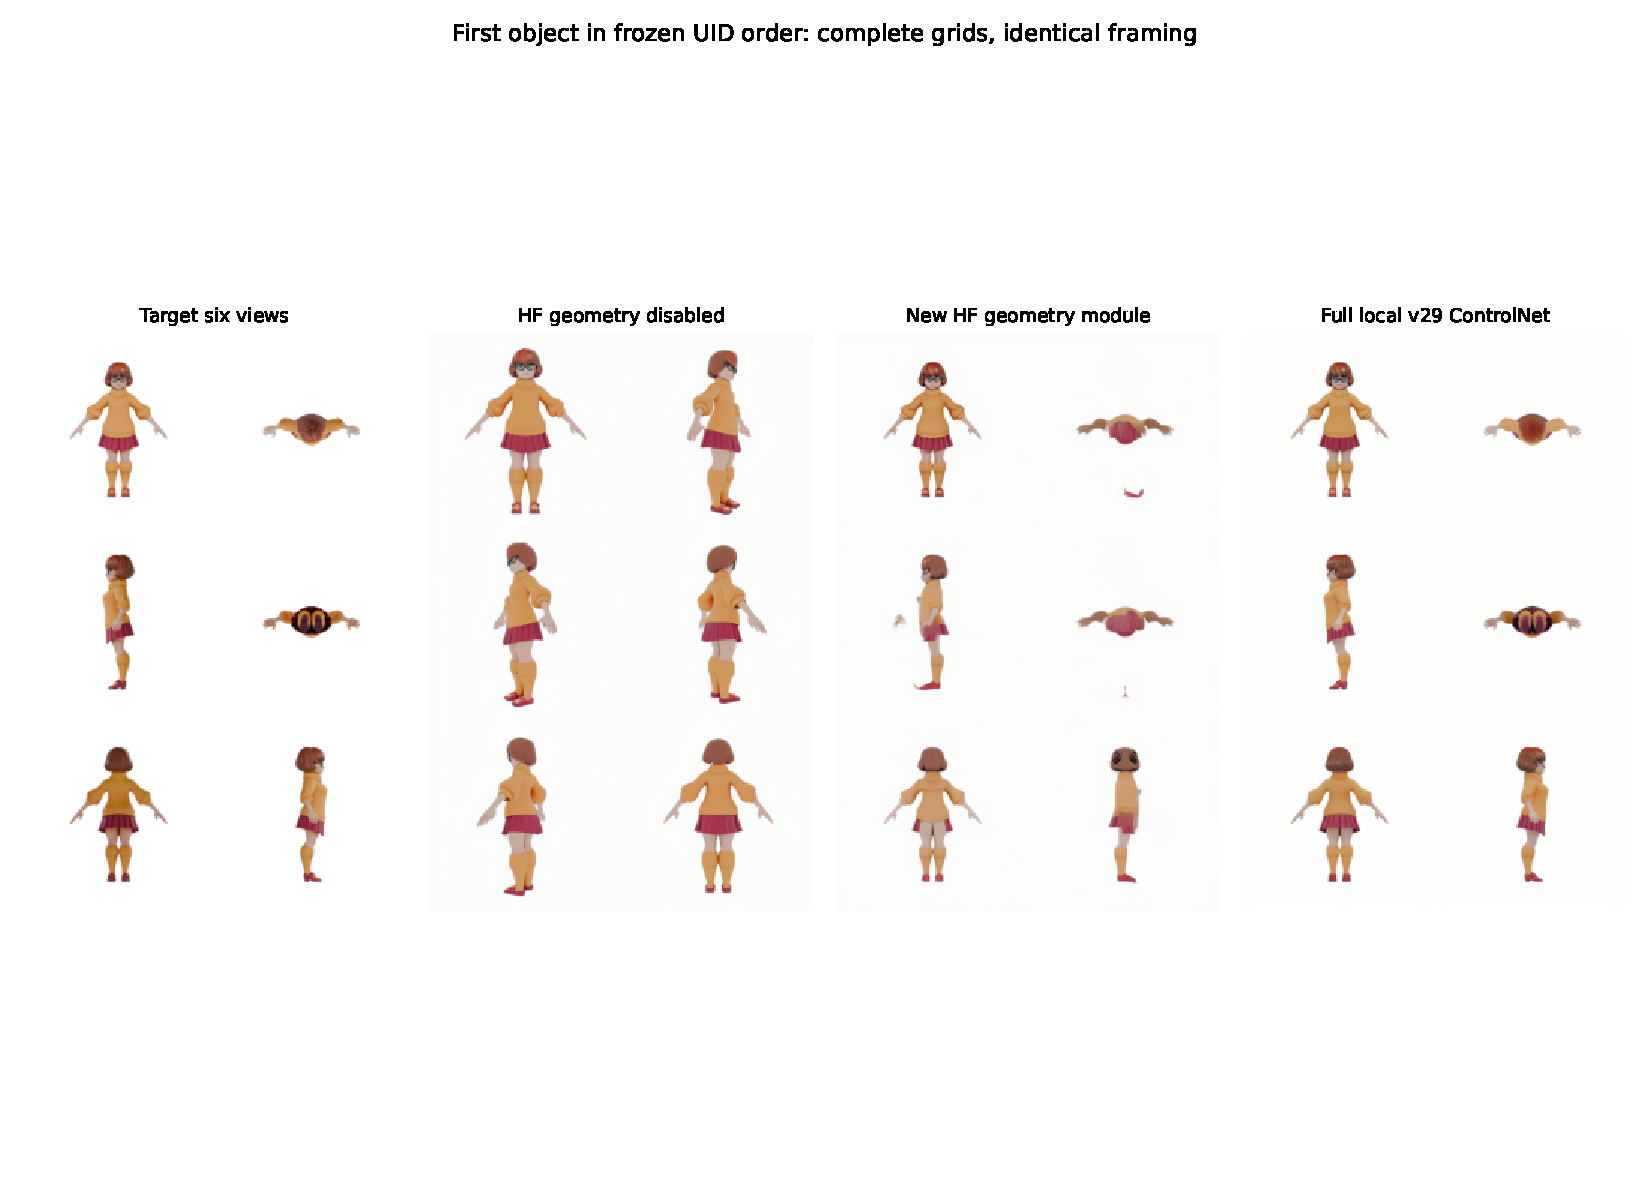
\includegraphics[width=\textwidth,height=0.74\textheight,keepaspectratio]{figures/figS9_native_checkpoint009.pdf}
\caption{Complete six-view grids for the first object in the frozen UID order, without output-based selection. These real outputs show why the weaker HF geometry-disabled comparison does not establish competitive performance against full v29. The new geometry module improves layout, while top/bottom semantic and reference-appearance failures remain. The target source view is included for context but excluded from the five-view inferential averages.}
\end{figure}

\subsection*{Same-v29-base training and frozen exploratory follow-up}\label{supp:samebase50}
\addcontentsline{toc}{subsection}{Same-v29-base training and frozen exploratory follow-up}
A subsequent same-base check exports all 1680 UNet tensors from the local converted v29 asset into an isolated pipeline, retaining the same CLIP/VAE assets and verifying every loaded UNet tensor at execution precision. Actual native positive/negative reference conditions match the existing cache on both GPUs. The same fixed 2000-update training protocol then completes, followed by the previously studied fifty-object cohort. Unscaled geometry improves FG-LPIPS relative to geometry disabled by 0.0131 (95\% interval $[-0.0189,-0.0083]$; 44/50 objects improve), but remains worse than full v29 by 0.0159 (interval $[0.0085,0.0237]$); both primary comparisons survive Holm correction. FG-SSIM also remains lower than full v29 by 0.0533 in the six-test secondary family. The PSNR and color differences are not separated after correction, which does not establish equivalence. Matching the base weights reduces a comparison confound but does not match geometry architectures, their training histories or all input representations. This exploratory follow-up reuses previously observed objects and neither demonstrates temporal-scheduling superiority nor establishes a competitive quality claim (S8).

The isolated UNet export leaves original HF and v29 assets unchanged. Tensor identity is checked after geometry wrappers are installed, removing wrapper naming only and excluding adapter tensors. An actual native first-call hook verifies positive/negative CLIP embeddings, reference VAE latents and added time IDs against the existing cached conditions for two fixed training objects on each GPU. A two-rank conditional/\allowbreak unconditional backward gate passes before formal training. The first gate fails before optimizer updates because a newly added reference-condition check uses the evaluation data root; the corrected check uses the configured training root, and the failed record is retained. This does not change the formal training cohort or remove an unfavorable output.

The formal run uses the same 1090 training objects, fixed final step 2000, seed policy, cache, losses and actual dropout as the preceding run. The evaluation retains all fifty previously inspected objects, with the same reference images, seeds, geometry targets and five nonreference endpoint averages. Reused full-v29 scores come from the identical fifty-object input protocol. Primary FG-LPIPS contrasts form a frozen Holm family of two; PSNR, SSIM and color differences for the two pairs form a separate family of six. The follow-up is frozen before this checkpoint's outputs, but is not an independent replication because previous cohort results motivated the base correction. Intervals are marginal paired object-bootstrap intervals, not simultaneous confidence intervals. No noninferiority threshold is chosen after the results.

\begin{center}\scriptsize
\begin{tabular}{llrrr}
\toprule
Comparison & Endpoint & Difference & 95\% interval & Holm $p$ \\
\midrule
Geometry -- disabled & fg\_lpips & -0.0131 & [-0.0189,-0.0083] & 0.00001 \\
Geometry -- full v29 & fg\_lpips & +0.0159 & [+0.0085,+0.0237] & 0.00014 \\
Geometry -- disabled & fg\_psnr & +3.3589 & [+2.6276,+4.1863] & 0.00003 \\
Geometry -- disabled & fg\_ssim & +0.0275 & [+0.0135,+0.0460] & 0.00003 \\
Geometry -- disabled & ciede2000 & -5.6605 & [-7.6065,-4.1823] & 0.00003 \\
Geometry -- full v29 & fg\_psnr & -0.8542 & [-1.6642,-0.0165] & 0.10169 \\
Geometry -- full v29 & fg\_ssim & -0.0533 & [-0.0711,-0.0352] & 0.00003 \\
Geometry -- full v29 & ciede2000 & -0.6506 & [-1.9014,+0.5307] & 0.30864 \\
\bottomrule
\end{tabular}

\end{center}
\begin{figure}[p]\centering
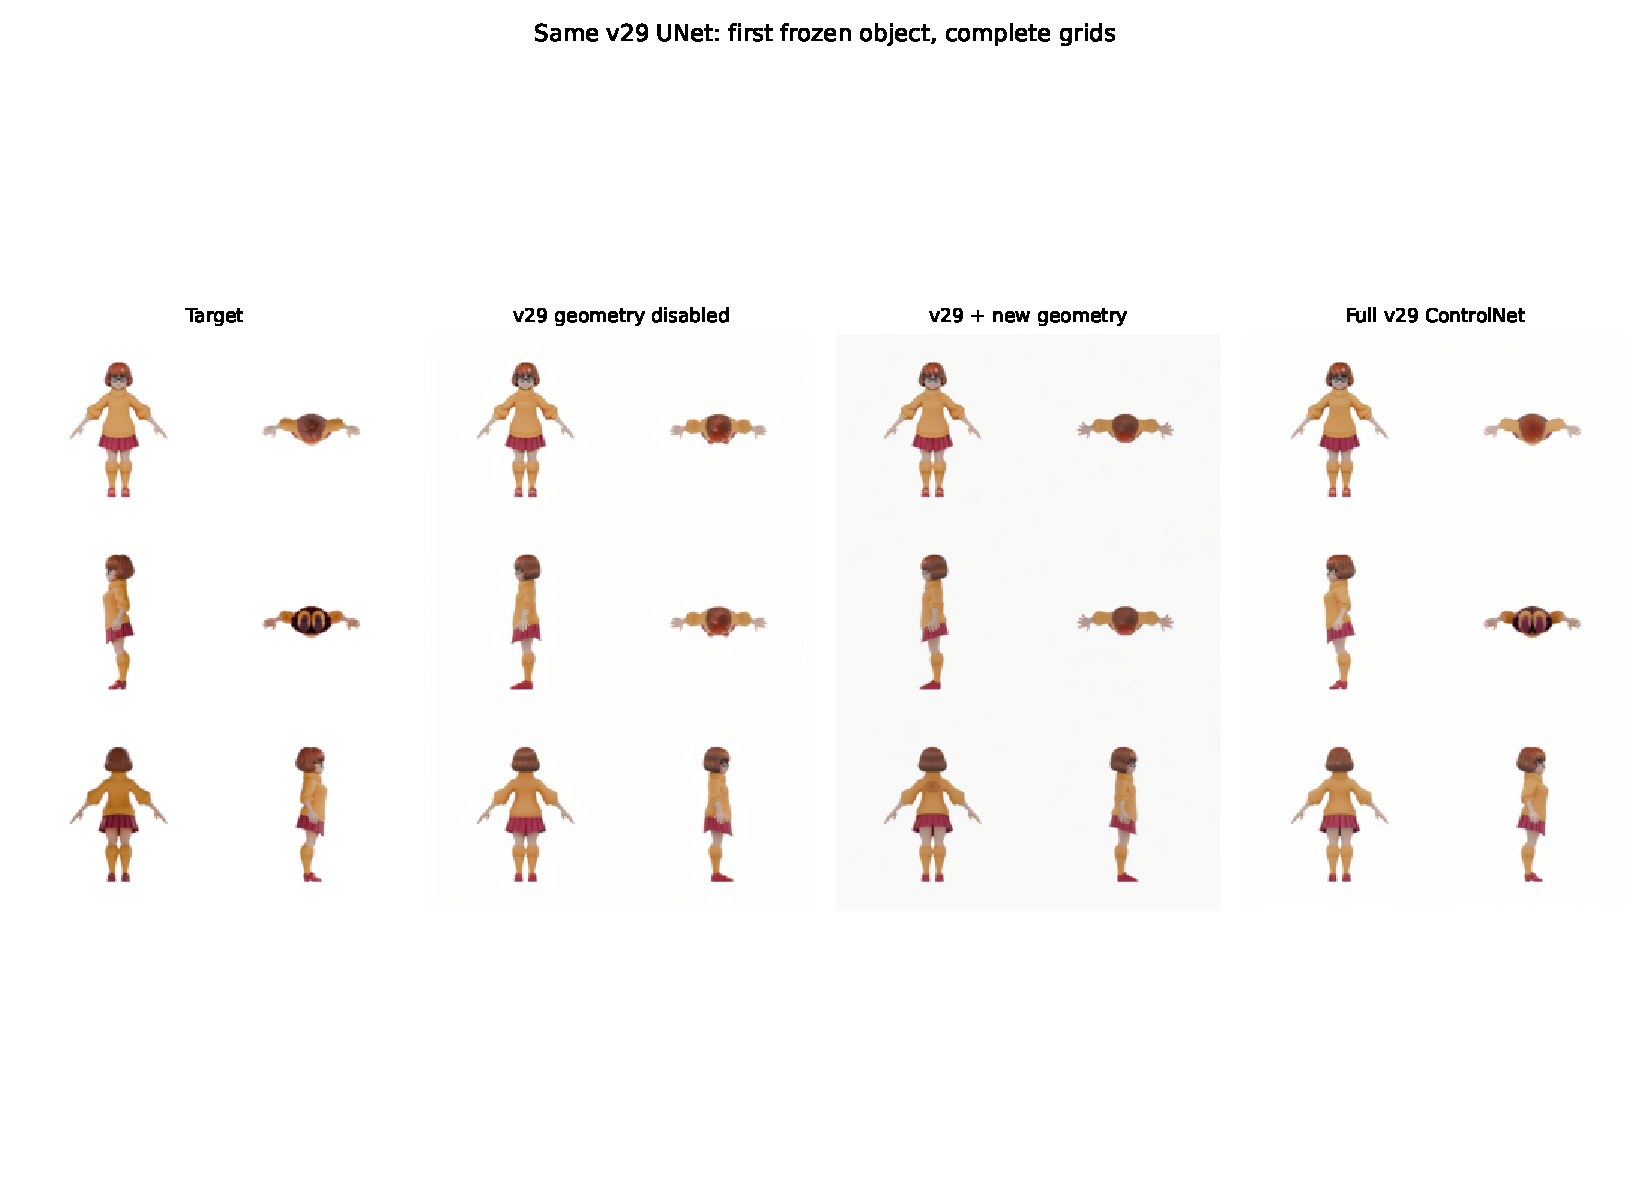
\includegraphics[width=\textwidth,height=0.74\textheight,keepaspectratio]{figures/figS10_same_base010.pdf}
\caption{Complete grids for the first frozen object under the same-v29-UNet follow-up. The full ControlNet baseline was generated in the preceding round with the same inputs. All fifty objects enter the paired analysis; this fixed example is not selected by quality. View placement and texture appearance remain mixed in the image endpoints.}
\end{figure}

\subsection*{Pixel-identical deployment performance}
\addcontentsline{toc}{subsection}{Pixel-identical deployment performance}
The performance protocol is frozen before timing. The first five UIDs in the fifty-object ordering are used without output-based selection. Phase 0 runs small geometry on GPU 0 and full v29 on GPU 1; phase 1 swaps them. Each process has its own resident pipeline, and the two GPUs share a CPU host during concurrent runs. This counterbalances card and order without removing every thermal or shared-host effect. Two first-object warm-ups precede fifteen timed calls per method/card. Geometry transfer and encoding, native reference preparation, denoising, VAE decoding and PIL conversion are inside the synchronized wall-time interval. Model load, disk input/output, CPU input-map construction and metric evaluation are outside it. No alternative precision, step count, reference cache or model compression is introduced.

All 68 calls, including eight warm-ups, match their previously evaluated output pixels exactly. Five saved PNGs per method/card independently verify this identity. The first full-v29 startup fails before generation because a resource guard is placed after this process creates its CUDA context; the corrected startup checks availability first and retains the failed attempt. Completed small-geometry records are reused, and no unfavorable timing or object is dropped. Per-GPU summaries and all raw timings are packaged. Peak allocated and reserved memory are both recorded; the main table reports allocated memory. Parameter counts include the base denoiser and geometry branch but exclude shared image encoders and VAE. Performance summaries are descriptive; repetitions do not increase the independent object count beyond five.

\begin{center}\scriptsize
\begin{tabular}{llrrrr}
\toprule
GPU & Deployment & Median (s) & Peak (GiB) & FG-LPIPS & FG-SSIM \\
\midrule
0 & Full v29 & 15.71 & 14.89 & 0.0775 & 0.6937 \\
0 & Small geometry & 12.03 & 13.18 & 0.0934 & 0.6404 \\
1 & Full v29 & 14.58 & 14.89 & 0.0775 & 0.6937 \\
1 & Small geometry & 11.17 & 13.18 & 0.0934 & 0.6404 \\
\bottomrule
\end{tabular}

\end{center}
The lower cost does not offset the measured quality loss by statistical fiat. No noninferiority bound or application utility function is introduced after observing results, and the architecture cost is not attributed to temporal scheduling.

\subsection*{Archived projection development and first-interface evaluation}
\addcontentsline{toc}{subsection}{Archived projection development and first-interface evaluation}
This section records completed development and first-interface confirmation
observations and external-input comparisons. The full fixed twenty-object bake evaluation is completed and reported in Supplementary Section~S4. The development matrix comprises 32 previously
studied objects per interface, four conditions, and three sampling seeds
(42, 2026, 31415), for 384 object--condition--seed cells per interface. The two
interfaces use different object sets and are not pooled as paired subjects.
Sampling seeds do not estimate training-checkpoint variation.

For matched noisy latents, let $f_u,f_c$ denote negative/positive conditional
predictions with geometry and $b_u,b_c$ the corresponding predictions without
geometry. Define $a=b_c-b_u$, $g_0=f_u-b_u$, and
$h=(f_c-f_u)-a$. The native guided prediction is $b_u+g_0+s(a+h)$.
The development interaction candidate removes the negatively parallel component
of $h$ along $a$ and retains $g_0$ algebraically. Total-geometry grid and
view projections are separate comparison conditions. These are operations in
noise-prediction space; $a$ is not a pure appearance-loss gradient. Algebraic
decomposition and vector projection alone do not establish method novelty.

On the unmodified first-interface seed-42 trajectories, 32 objects provide
50 observations each. The object-averaged cosine between the guided geometry
contribution and $a$ is $-0.6426$ (95\% object-bootstrap interval
$[-0.6611,-0.6235]$); all 1600 measured whole-grid rows are negative.
The auxiliary measurement preserves final native pixels exactly. This validates
measurement without disturbing the trajectory; negative cosine does not prove
that the geometry contribution harms final appearance. Two MV-Adapter objects
also show negative whole-object cosines at all 50 steps, with respective means
$-0.4965$ and $-0.4984$. Two objects do not establish population generalization.

Table~\ref{tab:development012} reports projection-minus-native differences on
first-interface development objects. Seeds and views are nested within objects;
intervals use 20,000 object-bootstrap resamples and are descriptive rather than
multiplicity-adjusted confirmatory tests. Source agreement improves, but the
nonreference LPIPS intervals cross zero. No noninferiority margin was specified,
and absence of a detected difference is not evidence of no quality loss.

\begin{table}[ht]
\centering\scriptsize
\begin{tabular}{lccc}
\toprule
Condition & Source FG-PSNR (dB) & Source $\Delta E_{00}$ & Nonreference FG-LPIPS \\
\midrule
Total geometry, grid & $+2.74$ $[+1.57,+3.97]$ & $-1.09$ $[-2.09,-0.38]$ & $-0.0016$ $[-0.0044,+0.0012]$ \\
Total geometry, view & $+3.01$ $[+1.80,+4.30]$ & $-1.16$ $[-2.16,-0.46]$ & $+0.0014$ $[-0.0017,+0.0047]$ \\
Interaction only, grid & $+2.79$ $[+1.56,+4.09]$ & $-1.06$ $[-2.07,-0.34]$ & $-0.0014$ $[-0.0046,+0.0017]$ \\
\bottomrule
\end{tabular}
\caption{Exploratory development differences and 95\% object intervals.
PSNR is higher-better; color difference and LPIPS are lower-better. All three
sampling seeds are averaged within each of the 32 objects. These are not new
independent confirmation objects.}
\label{tab:development012}
\end{table}

Second-interface reference-fidelity interpretation requires pose calibration. Native
view 0 has azimuth $-90^\circ$ and view 1 has azimuth $0^\circ$; source-view roles
cannot be transferred from the first interface by index alone. In the current
32-object set, eight target assets use a white texture fallback. The source-alpha
and candidate native-view-1 target masks have median pixel IoU 0.2606, so azimuth
agreement alone does not establish pixel registration. Earlier full-frame
reference comparison is also confounded by background: reference-alpha
background contributes a median 98.2\% of full-frame squared error for native
seed-42 view-1 outputs. A separate foreground/background-controlled diagnostic
has completed, but its pose-registration limitation prevents interpreting it as
validated reference fidelity or changing the confirmation endpoints.

\paragraph{Completed source-view confirmation and remaining tradeoffs.}
The 64-object, four-condition, three-seed matrix is complete (768 outputs).
The cohort excludes the 32 development objects but remains within historically
exposed Fresh C. The pre-generation specified view-projection versus native
comparisons give source FG-PSNR $+4.283$ dB (object-bootstrap 95\% CI
$[+3.409,+5.205]$; 61/64 object means favorable) and CIEDE2000 $-2.230$
($[-3.061,-1.563]$; 57/64 favorable). Both two-sided paired Monte Carlo
sign-flip tests have Holm-adjusted $p\approx 0.000010$ across the two primaries.
Seeds and views are nested within objects, not treated as independent samples.

Descriptive nonreference-view differences are FG-PSNR $-0.282$ dB
(pointwise 95\% CI $[-0.672,\allowbreak +0.102]$), FG-LPIPS $+0.000269$
($[-0.001533,\allowbreak +0.002073]$), CIEDE2000 $+0.425$
($[-0.157,\allowbreak +1.042]$), and FG-SSIM $+0.01062$
($[+0.00171,\allowbreak +0.01957]$). These secondary intervals are unadjusted.
Non-detection does not establish non-inferiority: no margin was specified.
The result confirms source-view gains for this comparison, not universal
multi-view gains, superiority of interaction projection, APG superiority,
or cross-interface transfer. APG's enabled norm-clipping path initially
failed because a matrix-norm operation received three reduction dimensions.
An explicit vector norm fixes that implementation error without changing the
frozen parameters; failed attempts are retained and the repaired APG matrix
and its scoring are now complete.

\paragraph{Completed APG and calibrated second-interface comparisons.}
On the same 32-object, three-seed first-interface development set, view
projection minus APG has nonreference FG-LPIPS $+0.000800$ for projection-only
APG (pointwise 95\% CI $[-0.002459,+0.004299]$) and $-0.000462$ for the
paper SDXL clipping/momentum preset at native CFG 2
($[-0.004354,+0.003482]$). Interaction projection gives $-0.002070$
($[-0.005351,+0.001259]$) and $-0.003331$
($[-0.007565,+0.000593]$), respectively. Holm correction across these four
specified development comparisons detects no advantage (adjusted
$p=1,1,0.7251,0.5100$). The paper preset is evaluated at the deployment CFG,
not the original paper's CFG 15; no preset was selected or tuned on these results.

The native-camera embedded-baseColor targets are distinct from the unregistered
reference-image domain discussed above. Re-rendering three input-selected
MV-Adapter objects reproduces all 18 archived RGBA target views exactly;
geometry-control masks and positions match the target render bitwise.
The full 32-object, four-condition, three-seed set can therefore be scored
against these native-camera targets, with no source/nonreference role inferred
from the view index. The all-six-view FG-LPIPS projection-minus-native
differences are $+0.000184$ (grid), $-0.000522$ (view), and $-0.000864$
(interaction). All pointwise intervals include zero and all three Holm-adjusted
$p$ values are 1. Eight white targets have legal constant-white embedded
baseColor; they remain in the full cohort, with the 24 textured objects reported
as a separate descriptive subset. This calibrated interface-specific endpoint
does not measure registered source-reference fidelity, physical albedo, or
final baked-texture quality.

\FloatBarrier
\clearpage
\section*{S9. Figure credits and additional displays}
\label{supp:group9}
\addcontentsline{toc}{section}{S9. Figure credits and additional displays}

\subsection*{Figure 2 sources and matched views}
\addcontentsline{toc}{subsection}{Figure 2 sources and matched views}
Main Figure 2 uses \emph{Green Iguan, re-created (not mine)} by dievitacola (\url{https://sketchfab.com/3d-models/1b0fd7f10ef84650bde143a4dba1a701}), \emph{Building 03} by Shalmon (\url{https://sketchfab.com/3d-models/building-03-c76ac44df995482185077da81939b306}), and \emph{Specimen 103} by jason.loxton (\url{https://sketchfab.com/3d-models/068ac3dfc34a464c89a5c467eb951969}), each licensed CC BY 4.0 (\url{https://creativecommons.org/licenses/by/4.0/}). Each row shows Target, Fixed Low, C3, Fixed High and Generic Linear from camera 000. Main Figure 3 source credits for Tire and the baptismal font are given in Section S5.

\subsection*{Current Fresh C figure credits}
\addcontentsline{toc}{subsection}{Current Fresh C figure credits}
The table records attribution for the Fresh C assets shown in the main and Supplementary figures.
\begin{longtable}{p{4.3cm}p{10.9cm}}
\caption{Attribution for Fresh C assets shown in the main text and Supplement.}\label{tab:supp-credits}\\
\toprule Display & Full attribution \\
\midrule\endfirsthead
\toprule Display & Full attribution \\
\midrule\endhead
Main Figure 4 & \emph{Cap Test -- PhotoCatch} by andrsbtrg, via Sketchfab (\url{https://sketchfab.com/3d-models/cap-test-photocatch-66ea60ce156e4815964dde27c196b9e5}), licensed CC BY 4.0 (\url{https://creativecommons.org/licenses/by/4.0/}). \\
Supplementary Figure~\ref{fig:supp-primary-examples}(a) & \emph{Building 03} by Shalmon, via Sketchfab (\url{https://sketchfab.com/3d-models/c76ac44df995482185077da81939b306}), licensed CC BY 4.0 (\url{https://creativecommons.org/licenses/by/4.0/}). Target-view RGB outputs share the same ROI and are arranged without color or detail adjustment. \\
Supplementary Figure~\ref{fig:supp-primary-examples}(b) & \emph{Boat Low Poly Game Ready} by INinja, via Sketchfab (\url{https://sketchfab.com/3d-models/d0e116a62bfc4cdd9edf60671073b306}), licensed CC BY 4.0 (\url{https://creativecommons.org/licenses/by/4.0/}). Target-view RGB outputs share the same ROI and are arranged without color or detail adjustment. \\
\bottomrule
\end{longtable}



\subsection*{Fresh C paired comparison examples}
\addcontentsline{toc}{subsection}{Fresh C paired comparison examples}
\begin{figure}[!t]
\centering
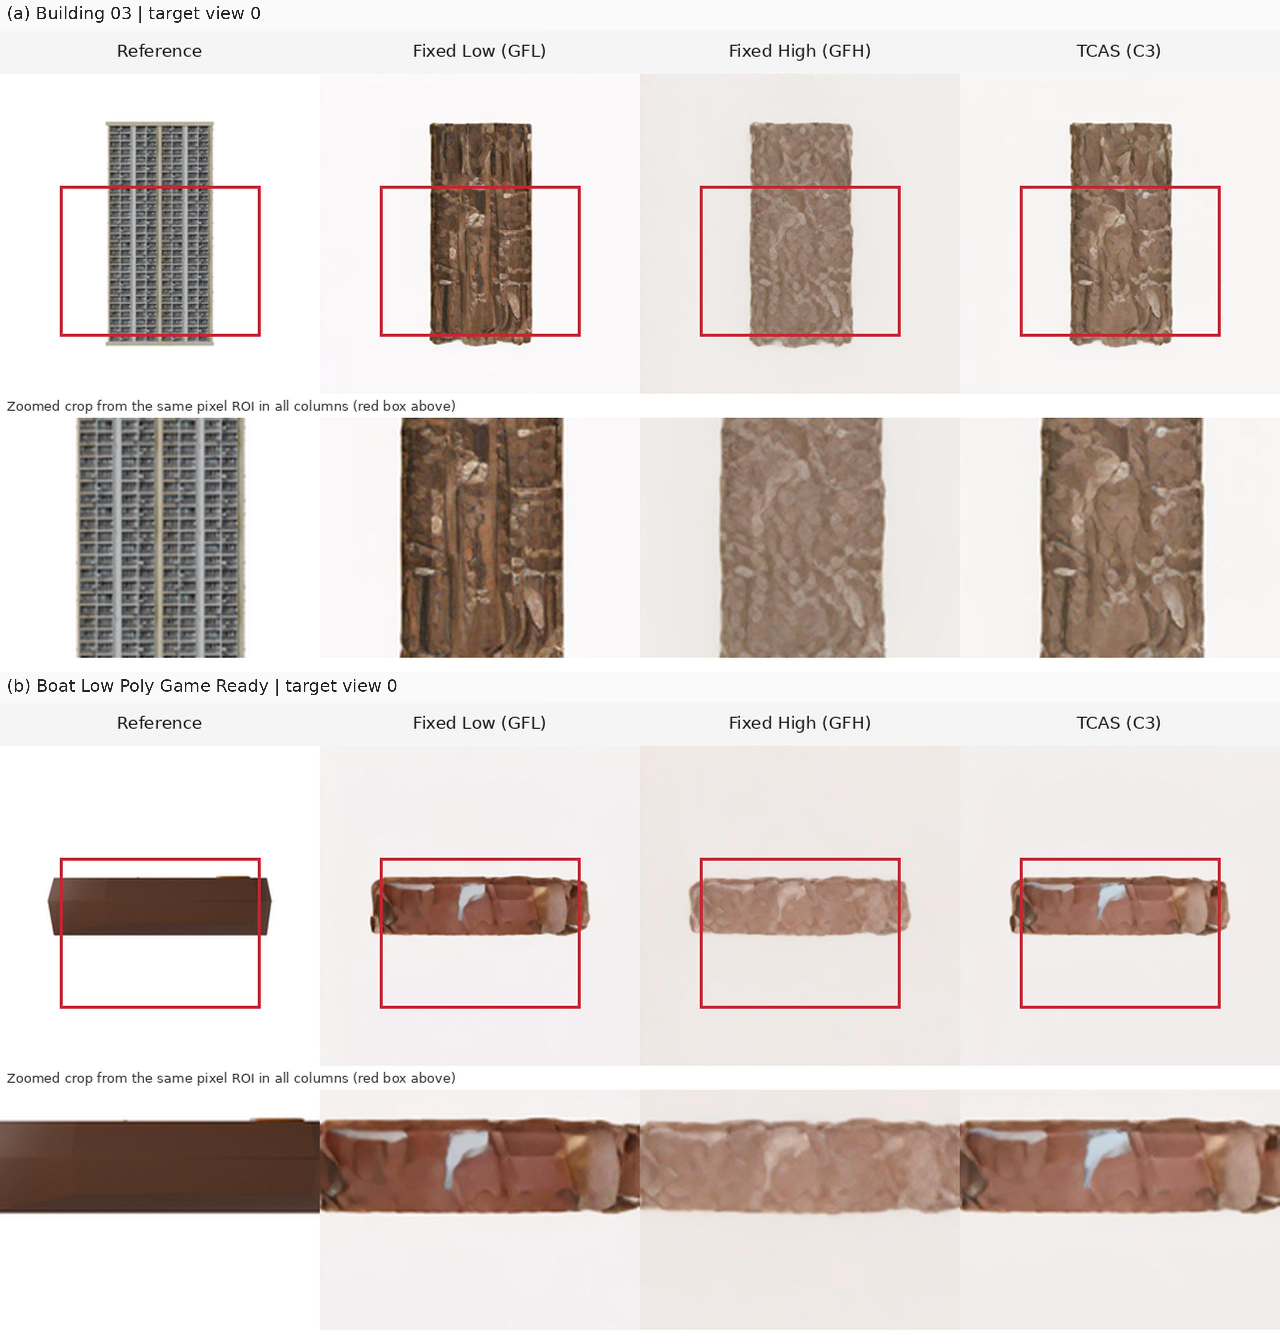
\includegraphics[width=\textwidth,height=0.74\textheight,keepaspectratio]{figures/fig4_freshc_context_roi_v5.pdf}
\caption{Matched Fresh C target-view RGB outputs for two objects under their shared reference, camera, checkpoint, runner, seed policy, and inference protocol. Each case pairs the full view, with the shared ROI marked in red, and its exact pixel crop. The comparison conditions are Reference, Fixed Low, Fixed High, and C3. Model credits are in Supplementary Section~S9.}
\label{fig:supp-primary-examples}
\end{figure}
\FloatBarrier






\clearpage
\section*{S10. Cross-branch experiment disposition}
\addcontentsline{toc}{section}{S10. Cross-branch experiment disposition}
This section summarizes historical and auxiliary attempts relevant to interpreting the current results. Their cohorts and endpoints are separate from the studies in S1--S8, and they do not add independent samples or confirmatory results.

\begingroup\small
\begin{longtable}{p{3.3cm}p{10.3cm}}
\caption{Relevant historical and auxiliary attempts and their evidence boundaries.}\\
\toprule Record family & Use and scientific boundary \\
\midrule\endfirsthead
\toprule Record family & Use and scientific boundary \\
\midrule\endhead
Historical fixed/layer/time searches & Old 24-object probes, old pooled 300-object extensions and strong-residual v2 panels explain development. Main v1 runtime identity remains incomplete; old favorable ranks are not an optimality argument. \\
Historical retraining and smokes & v2/v3/v4/v5, quick/extended and faithful/sweetspot directories have different configurations and completion evidence. Checkpoint existence is not a validated quality improvement; incomplete runs and NaN-update records remain listed. \\
FAC variants & Trained variants, frozen/penalized objectives and source-entry differences are retained as reported negative history in S7. Recovered components do not authenticate full historical training or imply that adaptive control generally fails. \\
A2/A3/A3b and scale diagnostics & Response heterogeneity, cap/stage tests, static-factorial and residual-budget feasibility remain auxiliary. Cross-layer raw-$L_2$ common-support evidence is withdrawn; no dose-independent mechanism is inferred. \\
TRB/TRB2 adaptive development & A separate old 24-object pilot failed promotion. TRB minus C3 FG-LPIPS is $+0.001302$ (pointwise interval $[+0.000079,+0.002549]$); after budget repair, TRB2 minus C3 is $-0.000045$ ($[-0.000827,+0.000670]$). The extra calibration pass adds cost, and no promoted 276 holdout was executed. This is development history, not a new winning algorithm. \\
Color-repair candidates & C1 failed visual inspection despite numerical changes; B2 improved only one of four development objects and failed its gate. Neither is incorporated into the final method or described as a validated repair. \\
Earlier native/camera/bake attempts & The old seven-object native quality panel and old five-object pole-mask/REPEAT evaluation have known calibration or sampling faults. Corrected records are separate; invalid results are not pooled with native50 or bake10. \\
Native training and full v29 & New 2,000-step checkpoints, complete fifty-object controls and same-base training quantify local quality/cost limits in S8. Architecture, weights and training differences are not attributed to TCAS scheduling. \\
Projection/APG and GSO & Complete source/nonreference, second-interface and three-seed matrices retain favorable, non-detected and adverse effects in S4/S8. Calibration failures and post hoc GT-only revisions remain explicit. \\
Other system attempts & Historical SF3D, Wonder3D and Hunyuan preparation records do not establish a matched same-task texture benchmark here. Missing identity, endpoint or completion chains are not supplied by output counts. \\
\bottomrule
\end{longtable}\endgroup

\end{document}
